\documentclass[fontsize=10pt,paper=b5,open=any,
twoside=yes,toc=listof,toc=bibliography,headings=optiontohead,
captions=nooneline,captions=tableabove,english,DIV=15,numbers=noenddot,final,parskip=half-,
headinclude=true,footinclude=false,BCOR=.5cm]{scrbook}
\pdfvariable suppressoptionalinfo 512\relax
\usepackage[bottom]{footmisc}
\raggedbottom
\usepackage{lualatex-math}
\usepackage{wrapfig2}
\usepackage{hirostyle}
\usepackage{hiromacros}

\newcommand{\figW}{\columnwidth}
\newcommand{\figH}{0.61803551232\figW}

\newcommand{\legendfontsize}{\tiny}
\newcommand{\tickfontsize}{\tiny}
\newcommand{\labelfontsize}{\scriptsize}


% \usepackage{verbatim} % provides the `\comment` block
% \renewenvironment{figure}[1][]{%
% \expandafter\comment%
% }{%
% \expandafter\endcomment%
% }
% \renewenvironment{wrapfig}[1][]{%
% \expandafter\comment%
% }{%
% \expandafter\endcomment%
% }


\usepackage[switch*]{lineno}
\renewcommand\linenumberfont{\normalfont\tiny\color{gray}}
\linenumbers


%% Patch 'normal' math environments:
\newcommand*\linenomathpatch[1]{%
  \cspreto{#1}{\linenomath}%
  \cspreto{#1*}{\linenomath}%
  \csappto{end#1}{\endlinenomath}%
  \csappto{end#1*}{\endlinenomath}%
}

\linenomathpatch{equation}
\linenomathpatch{gather}
\linenomathpatch{multline}
\linenomathpatch{align}
\linenomathpatch{alignat}
\linenomathpatch{flalign}

\addbibresource{references.bib}
\synctex=1
\title{Energy Flow in Strongly Coupled Open Quantum Systems}
\author{Valentin Boettcher}
\date{\today}

% \includeonly{./src/intro}

\begin{document}
\maketitle
\tableofcontents

% Chapters
\chapter{Introduction}
\label{chap:intro}
The field of quantum thermodynamics has attracted much
interest~\cite{Talkner2020Oct,Rivas2019Oct,Riechers2021Apr,Vinjanampathy2016Oct,Binder2018,Kurizki2021Dec}. Quantum
thermodynamics is, among other issues, concerned with extending the
standard phenomenological thermodynamic notions to microscopic systems
coupled to macroscopic baths. This setting may make it possible to
formulate rigorous microscopic definitions of thermodynamic quantities
such as internal energy, heat and work that are consistent with the
well-known laws of thermodynamics. There is no consensus on this
matter yet, as is demonstrated by the plethora of proposals and
discussions in
\cite{Rivas2019Oct,Talkner2020Oct,Motz2018Nov,Wiedmann2020Mar,Senior2020Feb,Kato2015Aug,Kato2016Dec,Strasberg2021Aug,Talkner2016Aug,Bera2021Feb,Bera2021Jun,Esposito2015Dec}.

The verification and evaluation of these issues in nontrivial
systems calls for an additional insight into the exact dynamics of
open quantum systems.  As system and baths may not be regarded as
separable entities in a strong coupling
regime~\cite{Rivas2019Oct,Esposito2015Dec} due to entanglement and
finite interactions strengths, access to the dynamics of system,
interaction and bath is required. This constitutes the fundamental
motivation for this work.

The exact treatment of strongly coupled and non Markovian open quantum
systems is a challenging problem.  If no analytical solution is
available, numerical methods have to be relied upon. Notably there are
pertubative methods such as the Redfield equations
\cite{Davidovic2020Sep} and also exact methods like the Hierarchical
Equations of Motion \emph{HEOM}~\cite{Tanimura1990Jun,Tang2015Dec},
multilayer MCTDH~\cite{Wang2010May}, TEMPO~\cite{Strathearn2018Aug}
and the Hierarchy of Pure States
\emph{HOPS}~\cite{Suess2014Oct}\footnote{See \cite{RichardDiss} for a
  detailed account.}. Although the focus of these methods is on the
reduced system dynamics, exact treatments of open systems can provide
access to the global unitary evolution of the system and the baths.

% In some settings
% \cite{Kato2016Dec,Lobejko2021Feb, Strasberg2021Aug}, such as cyclic
% heat engines, the change in the bath energies is a quite suitable
% definition of heat, as is expounded in
% \cref{sec:basic_thermo,sec:operational_thermo}.

In this work we will focus on the framework of the ``Non Markovian
Quantum State Diffusion'' (NMQSD)~\cite{Diosi1998Mar}, which will be
reviewed in~\cref{sec:open_systems,sec:nmqsd_basics}. We will show in
\cref{chap:flow} that the NMQSD allows access to interaction and bath
related quantities. This novel application of the formalism
constitutes the main result of this work.

Based on the NMQSD and inspired by the ideas behind HEOM a numerical
method, the ``Hierarchy of Pure States''
(HOPS)~\cite{RichardDiss,Hartmann2017Dec}, can be formulated and will
be briefly reviewed in \cref{sec:hops_basics}.

The results of \cref{chap:flow}, most importantly the calculation of
bath and interaction energy expectation values, can be easily
implemented within this numerical framework. By doing so we will
elucidate the role of certain features inherent to the method. The
most general case we will be able to handle is a system coupled to
multiple baths of differing temperatures under arbitrary
modulation. As HOPS on its own is already a method with a very broad
range of applicability~\cite{RichardDiss}, we will find it to be
suitable for the exploration of thermodynamical settings.

\Cref{chap:analytsol} is concerned with the analytical solution of the
well known model for Quantum Brownian Motion (QBM). This solution will
be applied to exactly calculate bath related quantities to provide a
benchmark for HOPS and the results of \cref{chap:flow}.

The implementation and systematic application of this benchmark is
performed in \cref{chap:numres}. Further, the spin boson model will be
explored as an example of a system that is not exactly solvable in
general. This also gives us the first opportunity to discuss and
explore the intricacies of the interplay between system, interaction
and bath energy expectation values, as well as the flow of energy
between system and bath.

Finally, we will turn to some thermodynamical questions in
\cref{sec:therm_results} both from a conceptual angle in
\cref{sec:basic_thermo} and through the exploration of concrete
systems in \cref{sec:singlemod,sec:otto}. Beginning with a review of
some bounds on energy extraction from systems coupled to infinite
baths the concept of ergotropy will be discussed and illustrated
through a concrete calculation. Importantly, this requires us to take
a perspective that is centered on the global unitary evolution which
we have access to with HOPS.  Subsequently, we will turn to
periodically modulated systems and explore both the capabilities of
HOPS, and the role of the aforementioned bounds in actual models.

The aim of this work is to demonstrate the validity of the HOPS
framework and its suitability for thermodynamical applications. In
this spirit quantum Brownian motion and spin-boson like models are
being explored to provide an overview of the capabilities of the
method and ideas for future studies. Although those are mentioned
throughout the work, some promising avenues are being highlighted in
\cref{cha:concl-ideas-future}.

\section{Open Quantum Systems}
\label{sec:open_systems}
Quantum physics' most important equation, the Schr\"odinger equation,
allows us to predict the future of a system knowing its initial state
if restrict ourself to pure states. Writing it down
\begin{equation}
  \label{eq:schroedinger}
  \iu ∂_{t} \ket{ψ(t)} = H \ket{ψ(t)},
\end{equation}
we find that we need only to specify a \emph{Hamiltonian} \(H\) that
acts on our system state which is an element of a Hilbert space of
some possible infinite dimension \(N\). Throughout the work we set
\(\hbar=c=1\).

We call the time evolution generated by \cref{eq:schroedinger}
\emph{Unitary}, as it preserves the norm of a state and is reversible.
Given any time independent Hamiltonian we may write down the time
evolution operator to solve the Schr\"odinger equation
\begin{equation}
  \label{eq:time_evo_op}
  U(t, t_{0})=\eu^{-\iu H (t-t_{0})},\; U(t, t_{0})^\dag U(t, t_{0}) =
  \id,\; U(t, t_{0})\ket{ψ(t_{0})} = \ket{ψ(t)}.
\end{equation}

For time independent Hamiltonians the Schr\"odinger equation describes
a closed system which constitutes, within the scope of the problem in
question, the whole universe. In general, it is very hard to find a
closed expression for \cref{eq:time_evo_op}, except for very special
cases. Either we recourse to approximations or we apply numerical
methods to solve \cref{eq:schroedinger}.

When the Hilbert space dimension is small, its numerical solution is
straight forward. But in more realistic scenarios we may still be
interested in a small system, but we cannot neglect the interaction of
that system with a much larger environment sometimes consisting of
infinite degrees of freedom. If the atmosphere of the earth would be
neglected when describing the descent of a space reentry capsule we
would arrive at fatally wrong results. Similarly, modern applications
of quantum physics deal with systems that undergo quantum evolution
under conditions that are not consistent with an isolated
system.

Specifically in quantum computing~\cite{Gill2022Jan}, the effect of
environmental interactions poses a major problem.  Also, in quantum
thermodynamics, we are often concerned with irreversible dynamics that
converge to a steady state or a limit cycle. This is only possible, if
the bath possesses infininite degrees of freedom \cite{Breuer2002Jun}.

As an example from the classical domain, Stokes drag models the
influence of a viscous fluid on spherical objects and can be
implemented by adding a velocity dependent term to the equation of
motion of our object,
\begin{equation}
  \label{eq:newton}
  \ddot{x} = F - α \dot{x}.
\end{equation}
We still retain all information about the system, the particle, having
accounted effectively for an environment, the fluid by introducing a
term that breaks energy conservation.

In quantum physics, we find that the situation is more complicated.
Writing down a Hamiltonian we have to account for both system and
environment in a composite Hilbert space
\(\hilb=\hilb_{\sys}\otimes\hilb_{\bath}\)
\begin{equation}
  \label{eq:general_open}
  H = H_{\sys} \otimes \id_{\bath} + \id_{\sys} \otimes H_{\bath} + H_{\inter},
\end{equation}
where \(\sys\) marks the system, \(\bath\) marks the environment (or
bath) and \(H_{\inter}\) models their interaction.

Although the global state of system and environment may be pure,
entanglement of system and environment leads to the effect, that we
may know the system state only as a statistical mixture of states
called the \emph{reduced state}. No part of a composite system may be
in general be known as ``precicely'' as the whole. This is a major
departure from classical physics.

Starting from a possibly mixed global state \(ρ(t)\) we find, that to
compute the dynamics of all observables \(O_{\sys}\) which only act on
the system Hilbert space it is sufficient to know
\(ρ_{\sys}(t)=\tr_{\bath}[ρ(t)]\), the reduced system state.

The partial trace \(\tr_{\bath}\) averages over all bath degrees of
freedom and removes them from explicit consideration. This is a very
useful device, as the environment usually has a Hilbert space
dimension that is much too large for practical
calculations. Especially in numerics this fact is important, as even
an environment consisting of \(40\) two level systems would consume
\(16\) tebibytes of memory when stored as double precision complex
floating point numbers.

We will discover in \cref{chap:flow} that although it is impractical
to work with the bath state directly, it is still possible gain access
to bath-global observables such as the change in the expectation value
of the bath energy.

Under certain assumptions, most importantly that of weak coupling
\(\ev{H_{\inter}}\approx 0\), a pertubative treatment of the
environment yields an evolution equation, called a \emph{master
  equation}, that only contains the system state
\(ρ_{\sys}\)~\cite[p. 115 ff.]{Breuer2002Jun,Rivas2012}, leading to
irreversible non unitary dynamics.

A special master equation often called
Gorini–Kossakowski–Sudarshan–Lindblad equation, or GKSL equation in
short, and has the form
\begin{equation}
  \label{eq:gksl}
  \dot{ρ}_{\sys} = -\iu \comm{H}{ρ_{\sys}} + \mathcal{D}[ρ_{\sys}] = \mathcal{L}[ρ_{\sys}],
\end{equation}
where \(\mathcal{D}\) is called the \emph{dissipator} which adds
non-unitary dynamics to the von Neumann equation and \(H\) is a
unitary contribution not necessarily equal to \(H_{\sys}\).

Integrating \cref{eq:gksl} leads to a map
\(ρ_{\sys}(t) = \mathcal{E}_{t}(ρ_{\sys}(0))\).  The evolution
generated by \cref{eq:gksl} is called Markovian, as
\(\mathcal{E}_{t+s}= \mathcal{E}_{t}\circ\mathcal{E}_{s}\). More
fundamentally, this is due to the fact that at some point one assumes,
that the bath has no ``memory''\footnote{This does not mean that the
  global state has always the form
  \(ρ_{\sys}(t)\otimes ρ_{\bath}(t)\)~\cite{Rivas2012}.}. Without
getting into details, one may say that the characteristic time scales
upon which correlation functions of bath observables decay should be
much smaller than the time scales of the system.

If one endeavors to drop the assumptions of weak coupling and of
Markovian dynamics, the situation becomes more complicated. But when
introducing a concrete model of the bath we find that
\cref{eq:schroedinger} can be recast into a form that allows for an
exact numerical solution. As alluded to above, the great advantage of
this exact approach is that although we solve for the reduced state
\(ρ_{\sys}\), we essentially compute the unitary dynamics of
system. Thus, we can additionally retain some information about the
bath which allows us to quantify the change in expected bath energy
and also the expectation value of the interaction Hamiltonian.

\Cref{sec:nmqsd_basics} will introduce the general model whose
solution will be made feasible with the introduction of the \emph{Non
  Markovian Quantum State Diffusion}. The numerical implementation of
the NMQSD, the \emph{Hierarchy of Pure States}, will be the topic of
\cref{sec:hops_basics}.

A more detailed account of both subjects can be found in
\cref{sec:multihops} as well as \cite{RichardDiss}.


\section{The Non Markovian Quantum State Diffusion (NMQSD)}
\label{sec:nmqsd_basics}

We will now introduce the most general form of the models that will be
discussed in this thesis. This model has a wide applicability and many
microscopic systems can be cast into its form
\cite{Strunz2001Habil}\cite[chap. 2]{RichardDiss}, although there
certainly exist limits of applicability~\cite{Caldeira2014Mar}.

Consider a general quantum system \(H_\sys(t)\) coupled to \(N\) baths
of harmonic oscillators\footnote{For instance, the electromagnetic field.}
\begin{equation}
  \label{eq:generalmodel}
  H(t) = H_\sys(t) + ∑_{n=1}^N \qty[L_n^†(t)B_n + \hc] + ∑_{n=1}^NH_B\nth ,
\end{equation}
with \(B_n=∑_{λ} g_λ\nth a_λ\nth\) and
\(H_B\nth=∑_λω_λ\nth \qty(a_λ\nth)^\dag a_λ\nth\). The \(a_λ\nth\) are
bosonic annihilation operators acting on \(n\)th bath Hilbert space
and the \(L_n\) are arbitrary not necessarily hermitian operators
acting on the system Hilbert space. Quite general baths can be mapped
to this model in the thermodynamic limit, when the bath consists of an
infinite number of independent systems as was shown in
\cite{Makri1999Apr}.

Despite the simple structure of the baths, \cref{eq:generalmodel} is
generally very hard to solve beyond weak coupling strengths as has
been detailed in~\cref{sec:open_systems}. The ``Non Markovian Quantum
State Diffusion'' \cite{Diosi1998Mar} approach allows to
recast \cref{eq:generalmodel} into a stochastic differential equation
in which the bath degrees of freedom are accounted for by Gaussian
stochastic processes and a memory term.

Here we only consider a single zero temperature bath initially in the
ground state \(\ket{0}\). For more complete and general account see
\cite{RichardDiss,Strunz2001Habil,Diosi1998Mar,Hartmann2017Dec,Hartmann2021Aug}
and \cref{sec:hops_multibath}.

The total system-bath state may then be expanded in a Bargmann
unnormalized coherent state basis~\cite{klauder1968fundamentals} with
respect to the bath degrees of freedom
\begin{equation}
  \label{eq:projected_single}
  \ket{ψ(t)} = ∫{\frac{\dd{\vb{z}}}{π^{N}}\eu^{-\abs{\vb{z}}^2}}\ket{ψ(t,\vb{z}^\ast)}\ket{\vb{z}},
\end{equation}
where \(\vb{z}\) is a vector of coherent state labels \(z_λ\) for each
environment oscillator. The reason for using unnormalized coherent
states is that this leads to \(\ket{ψ(t,\vb{z}^{\ast})}\) being a
holomorphic function of \(\vb{z}^\ast\).


After transforming \cref{eq:generalmodel} into the interaction picture
with respect to \(H_\bath\) and using the properties of the coherent
states (\(\mel{z_λ}{a_λ}{ψ}\rightarrow ∂_{z_λ^\ast}\braket{z_λ}{ψ}\),
\(\mel{z_λ}{a_λ^\dag}{ψ}\rightarrow z_λ^\ast\braket{z_λ}{ψ}\)) we
arrive at an equation for \(\ket{ψ(t,\vb{z}^{\ast})}\)
\begin{equation}
  \label{eq:nmqsd_single_proto}
  ∂_t\ket{ψ(t,\vb{z}^{\ast})} = -\iu H \ket{ψ(t,\vb{z}^{\ast})} - \iu
  L ∑_{λ}g_{λ}^\ast z_{λ}^\ast \eu^{\iu ω_{λ} t}
  \ket{ψ(t,\vb{z}^{\ast})} - \iu L^\dag ∑_{λ} g_{λ}\eu^{-\iu ω_{λ} t}\pdv{}{z_{λ}^\ast}\ket{ψ(t,\vb{z}^{\ast})}.
\end{equation}

From this point on there are multiple avenues open to us. We choose
the canonical one of \cite{Strunz2001Habil}, but there is also a
time-discrete derivation that avoids functional derivatives
in~\cite{Hartmann2021Aug}.

We shift the perspective and define~\cite{RichardDiss,Strunz2001Habil}
\begin{equation}
  \label{eq:single_process}
  η^\ast_{t} = -\iu ∑_λg_λ^{\ast} z_λ^{\ast}\eu^{\iu ω_λ t}.
\end{equation}
Using
\(\pdv{z_λ^{\ast}}=∫\dd{s}\pdv{η^\ast_{s}}{z_λ^{\ast}}\fdv{η^\ast_{s}}\)
and interpreting \(\ket{ψ(t,\vb{z}^{\ast})}\) as a functional of
\(η_{t}^\ast\) we arrive at
\begin{equation}
  \label{eq:nmqsd_single}\tag{NMQSD}
  ∂_t\ket{ψ(η^\ast_t, t)} = -\iu H \ket{ψ(η^\ast_t, t)} +
  L {η}^\ast_t\ket{ψ({η}^\ast_t, t)} -
  L^†∫_0^t\dd{s}α(t-s)\fdv{\ket{ψ({η}^\ast_t, t)}}{η^\ast_s},
\end{equation}
where \(α\) is the zero temperature bath correlation function (BCF)
\begin{equation}
  \label{eq:bcfdef}
  α(t-s) = ∑_λ \abs{g_λ}^2\eu^{-\iu ω_λ (t-s)}
\end{equation}
and \(η_t\) is a Gaussian stochastic process obeying
\begin{equation}
  \label{eq:single_processescorr}
  \begin{aligned}
      \mathcal{M}(η_t) &=0, & \mathcal{M}(η_tη_s) &= 0,
      & \mathcal{M}(η_tη_s^\ast) &= α(t-s).
  \end{aligned}
\end{equation}
The functional \(\ket{ψ(η_{t}^\ast)}\) is essentially the state of the
system relative to some coherent bath state, encoded in the value of
the stochastic process.

The statistics of the process follow from interpreting
\cref{eq:projected_single} in a Monte-Carlo sense and thus the reduced
system state may then be recovered by averaging over all trajectories
\begin{equation}
  \label{eq:recover_rho}
  ρ_{\sys}(t) = \tr_{\bath}\bqty{\ketbra{ψ(t)}} =
 ∫{\frac{\dd{\vb{z}}}{π^{N}}\eu^{-\abs{\vb{z}}^2}}\ketbra{ψ(t,\vb{z})}{ψ(t,\vb{z}^\ast)}=
  \mathcal{M}_{η_{t}^\ast}\bqty{\ketbra{ψ(η_t, t)}{ψ(η^\ast_t, t)}}.
\end{equation}

Note that the BCF \(α\) relates to the so called spectral density
\begin{equation}
  \label{eq:specdens}
  J(ω) = {π} ∑_λ \abs{g_λ}^2 δ(ω-ω_λ)
\end{equation}
via the Fourier transform.

One then usually performs a continuum limit so that \(J(ω)\) becomes
``smeared out'' to a smooth function and \(α(τ)\) decays to zero for
\(τ\rightarrow ∞\).

The NMQSD formalism shows that we can treat an infinite environment
with a stochastic differential equation in which only objects of
system dimension appear. Note also, that we can allow an explicit time
dependence of \(L\) and \(H\) without alterations to
the NMQSD.

Equation \cref{eq:nmqsd_single} does not preserve the norm of the
state, leading to suboptimal convergence of \cref{eq:recover_rho}.
When recovering the system state, we would like to average over
normalized states
\begin{equation}
  \label{eq:norm_av}
  ρ_{\sys}(t) =
 ∫{\frac{\dd{\vb{z}}}{π^{N}}\eu^{-\abs{\vb{z}}^2}}
 \braket{ψ(t,\vb{z})}{ψ(t,\vb{z}^\ast)} \frac{\ketbra{ψ(t,\vb{z})}{ψ(t,\vb{z}^\ast)}}{\braket{ψ(t,\vb{z})}{ψ(t,\vb{z}^\ast)}}.
\end{equation}

This can be achieved~\cite{RichardDiss,Suess2014Oct} by using a
co-moving shifted stochastic process
\begin{equation}
  \label{eq:shifted_proc}
  \tilde{η}_{t}^\ast= η^\ast_{t} + ∫_{0}^{t}\dd{s} α^\ast(t-s) \ev{L^\ast}_{s},
\end{equation}
where
\(\ev{L^\dag}_{t}=\mel{ψ(\tilde{η}_{t}, t)}{L^\dag}{
ψ(\tilde{η}_{t}^\ast,t)}\). The origin of this shift lies in the
study of the Husimi \(Q\) function~\cite{Cartwright1976Jan} of the
bath
\(Q_{t}(\vb{z}, \vb{z}^\ast) = \eu^{-\abs{z}^{2}} π^{-N}
\braket{ψ(t,\vb{z})}{ψ(t,\vb{z}^\ast)}\). Shifting the process, or on
a deeper level the stochastic state labels, amounts to importance
sampling for each time step.

This leads to the nonlinear NMQSD equation~\cite{Diosi1998Mar}
\begin{equation}
  \label{eq:nmqsd_nonlin_single}
  ∂_t\ket{ψ(\tilde{η}^\ast_t, t)} = -\iu H \ket{ψ(\tilde{η}^\ast_t, t)} +
  L {\tilde{η}}^\ast_t\ket{ψ(\tilde{η}^\ast_t, t)} - \pqty{L^†
    -\ev{L^\dag}_{t}}∫_0^t\dd{s}α(t-s)\fdv{\ket{ψ({\tilde{η}}^\ast_t, t)}}{\tilde{η}^\ast_s}.
\end{equation}
There is a subtlety concerning the functional derivative that won't be
discussed here but in \cite{Hartmann2021Aug,RichardDiss} or
\cref{sec:nonlin_flow}.  Crucially, the system state is now recovered
through
\begin{equation}
  \label{eq:recover_rho_nonlinear}
  ρ_{\sys}(t) =
  \mathcal{M}_{\tilde{η}_{t}^\ast}\bqty{\frac{\ketbra{ψ(\tilde{η}_t, t)}{ψ(\tilde{η}^\ast_t,t)}}{\braket{ψ(\tilde{η}_t, t)}{ψ(\tilde{η}^\ast_t,t)}}},
\end{equation}
so that all trajectories contribute with ``equal weight''.

\section{The Hierarchy of Pure States (HOPS)}
\label{sec:hops_basics}
The equation \cref{eq:nmqsd_single} has removed the bath degrees of
freedom from explicit consideration, replacing them with a Gaussian
stochastic process and a rather complicated term containing a memory
integral and a functional derivative
\begin{equation}
  \label{eq:complicated_term}
  ∫_0^t\dd{s}α(t-s)\fdv{\ket{ψ({η}^\ast_t)}}{η^\ast_s}.
\end{equation}

There exist analytical approaches to this
term~\cite{Diosi1998Mar,Strunz2001Habil}, but we keep the approach as
general as possible and instead choose a numerical avenue.

They
key~\cite{Suess2014Oct,Hartmann2017Dec,Hartmann2021Aug,RichardDiss} is
to cast the complicated term containing the functional derivative into
an auxiliary state. Expanding the BCF into exponentials\footnote{See
  \cite{RichardDiss,Hartmann2021Aug} for a detailed account of the
  systematics of this expansion.}
\(α(τ)=∑_{μ}G_{μ=1}^{M}\eu^{-W_{μ}τ}\) and defining
\begin{equation}
  \label{eq:d_op_one}
  D_{μ}(t)\equiv ∫_{0}^{t} G_{μ} \eu^{-W_{μ}(t-s)} \fdv{η^\ast_s}\dd{s},\; D^{\vb{k}}(t)\equiv \prod_{μ=1}^{M}\sqrt{\frac{k_{μ}!}{G_{μ}^{k_{μ}}}}
  \frac{1}{i^{k_{μ}}}\pqty{D_{μ}}^{k_{μ}}
\end{equation}
we can define the \(\vb{k}th\) hierarchy state
\begin{equation}
  \label{eq:d_op_hier}
  \ket{ψ^{\vb{k}}}\equiv D^{\vb{k}}\ket{ψ}.
\end{equation}

The origin of the normalization chosen in \cref{eq:d_op_hier} is the
desire to give all hierarchy states the same unit and to formulate the
final hops equations unified into one equation in an enlarged Hilbert
space~\cite{Gao2021Sep}. We refrain from going into details here and
refer to \cref{sec:multihops} instead.

For this state the following equation of motion can be
derived~\cite{Suess2014Oct,Hartmann2021Aug}
\begin{equation}
  \label{eq:singlehops}\tag{HOPS}
  \ket{\dot{ψ}^{\vb{k}}} = \qty[-\iu H_\sys + \vb{L}\cdot\vb{η}^\ast -
  ∑_{μ=1}^{M}k_{μ}W_μ]\ket{ψ^{\vb{k}}} +
  \iu ∑_{μ=1}^{M}\sqrt{G_μ}\qty[\sqrt{k_{μ}}  L \ket{ψ^{\vb{k} -
    \vb{e}_{μ}}} + \sqrt{\qty(k_{μ} + 1)}  L^† \ket{ψ^{\vb{k} +
    \vb{e}_{μ}}} ],
\end{equation}
where \(\vb{k}=(k_{1}, k_{2}, \ldots, k_{M})\) with \(k_{μ}\geq 0\) is
a multi index and \(\pqty{\vb{e}_{μ}}_{ν} = δ_{μ,ν}\). The term
\({\vb{k} - \vb{e}_{μ}}\) is evaluated only if \(k_{μ}\geq 1\). The
norm of the multi index \(\vb{k}\) is denoted
\(\abs{\vb{k}}=∑_{μ}k_{μ}\) and called the hierarchy level of
\(\ket{ψ^{\vb{k}}}\). The state
\(\ket{ψ(η_{t}^\ast, t)}\equiv \ket{ψ^{\vb{0}}}\) corresponds to the
trajectory obeying \cref{eq:nmqsd_single}.


We call \cref{eq:singlehops} the \emph{Hierarchy of Pure States}
because each hierarchy state couples only to the hierarchy states one
level above and one level below. This is similar to the
\emph{Hierarchical Equations of Motion} (HEOM) approach used
in~\cite{Kato2016Dec}, but with the advantage of reducing the
dimensionality from \(\dim{\hilb_{\sys}}^{2}\) to
\(\dim{\hilb_{\sys}}\) by treating pure states instead of density
matrices.

By truncating the hierarchy we obtain from \cref{eq:singlehops} a
system of time linear differential equations with time dependent
coefficients that can be solved numerically. By choosing a suitable
cutoff the method can be made arbitrarily
exact~\cite{Hartmann2021Aug}. For concrete truncation schemes see~
\cite{RichardDiss,Zhang2018Apr,Hartmann2021Aug} and
\cref{sec:truncsch}. In most simulations in this work the so called
\emph{simplex truncation scheme} was used. This scheme amounts to only
including hierarchy states with \(\abs{\vb{k}} \leq k_{\max}\).

Note that the hierarchy states have no physical interpretation, but
can be thought of as the ``memory'' of the system. We will find in
\cref{chap:flow} that they can be of use beyond the mere calculation
of \(\ket{ψ}=\ket{ψ^{\vb{0}}}\).

The nonlinear NMQSD \cref{eq:nmqsd_nonlin_single} can be accommodated
in much the same way, except for the replacements
\(L^\dag\rightarrow \pqty{L^\dag-\ev{L^\dag}_{t}}\) and
\(η\rightarrow \tilde{η}\) in \cref{eq:singlehops} transforming it
into a \emph{nonlinear} system of differential
equations~\cite{Suess2014Oct}. Throughout this work, the nonlinear
method is being used, as it offers much superior convergence.

\section{A Note on Tooling}
\label{sec:note-tooling}

The source codes for the simulations presented in this work span
multiple repositories. They all make heavy use of
\texttt{Numpy}~\cite{harris2020array} and
\texttt{Scipy}~\cite{2020SciPy-NMeth}. Further the
\texttt{Arb}~\cite{Johansson2017arb} is employed for its excellent
implementation of special functions. A small contribution was made to
\texttt{Arb}s \texttt{python} bindings in the course of this work.

The main code repository for this work can be found under
\url{https://github.com/vale981/master-thesis}.

The directory \path{python/energy_flow_proper} contains several
project subdirectory with literate programming notebooks in the
\texttt{org} format~\cite{EricSchulte2022Sep}. A detailed listing
linking subprojects to chapters can be found in
\cref{tab:code_structure}.

\begin{table}[htp]
  \centering
  \begin{tabular}{ll}
    Directory & Application \\
    \midrule
    \path{07_one_bath_systematics} & \cref{sec:prec_sim} \\
    \path{08_dynamic_one_bath} & \cref{sec:singlemod} \\
    \path{09_dynamic_two_bath_one_qubit} & \cref{sec:otto} \\
    \path{10_antizeno_engine} & Reproduction of~\cite{Mukherjee2020Jan}, not in this work. \\
    \path{11_new_ho_comparison} & \cref{sec:hopsvsanalyt}
  \end{tabular}
  \caption{\label{tab:code_structure}\small The subprojects in the main
    repository and their application.}
\end{table}

Code implementing the results of \cref{chap:flow,chap:analytsol} can
be found under \url{https://github.com/vale981/hopsflow}. The models
discussed in \cref{chap:numres,sec:therm_results} are implement in
\url{https://github.com/vale981/two_qubit_model}.

Some modifications were made to the code that generates the stochastic
processes for HOPS. These modifications can be found under
\url{https://github.com/vale981/stocproc}, although they are mostly
merged into the original repository
\url{https://github.com/cimatosa/stocproc} of Richard Hartmann
\orcidlink{0000-0002-8967-6183}.

The extensive and well tested existing HOPS code of the Theoretical
Quantum Optics group\footnote{Available upon reasonable request.} was
created by Richard Hartmann. Some improvements have been made in the
course of this work this work.  Documentation, type hints and unit
tests have been introduced. The parallelization mechanism was
overhauled and now uses the \href{https://www.ray.io}{\texttt{Ray}}
library. The structure of the code was further modularized, allowing
for a simple implementation of new integration methods. Time dependent
couplings and multiple baths were added to the implementation.

The source code of this document is available under
\url{https://github.com/vale981/master-thesis-tex}.

\chapter{Bath Observables in NMQSD and HOPS}%
\label{chap:flow}
After setting the stage for open systems and introducing the prime
tools of this work, the NMQSD and HOPS, in \cref{chap:intro}, we will
now return to our original goal, the calculation of bath related
quantities. Although the NMQSD is a method for the reduced system
state, we still treat the full unitary dynamics of system and bath and
may expect that some information about the bath is retained.

In \cref{sec:flow_lin} we will begin by deriving an expression for the
bath energy change \(-∂_{t}\ev{H_{B}}\). Subsequently we will
generalize this result to the nonlinear theory in
\cref{sec:nonlin_flow} and to finite temperatures in
\cref{sec:lin_finite}. Yet a more general class of observables can be
treated with the methods that will be developed as is shown in
\cref{sec:general_obs}.

The generalization to multiple baths (\cref{sec:multibath}) and time
depend Hamiltonians (\cref{sec:timedep}) will present itself as
straight forward.

\section{Bath Energy Change of a Zero Temperature Bath}%
\label{sec:flow_lin}

In this section we demonstrate upon the example of the change of the
bath energy
\begin{equation}
  \label{eq:heatflowdef}
  J = - \dv{\ev{H_\bath}}{t}
\end{equation}
how collective bath observables may be obtained from the formalism
presented in \cref{sec:nmqsd_basics,sec:hops_basics}. We have adorned
\cref{eq:heatflowdef} with a negative sign and henceforth call this
quantity the bath energy flow or simply flow, as it constitutes the
flow of energy out of the bath into system and interaction.

The simplest version of the general model \cref{eq:generalmodel} is
given by
\begin{equation}
  \label{eq:totalH}
  H = H_\sys + \underbrace{LB^† + L^† B}_{H_\inter} + H_\bath
\end{equation}
with the system hamiltonian \(H_\sys\), the bath Hamiltonian
\(H_\bath = ∑_\lambda ω_\lambda a_{λ}^† a_{λ}\), the bath coupling
system operator \(L\) and the bath coupling bath operator
\(B=∑_{\lambda} g_{\lambda} a_{\lambda}\) which define the interaction
Hamiltonian \(H_\inter\).

We do not consider external modulation of the Hamiltonian, finite
temperatures or multiple baths at this stage, as we are interested in
the essentials of the procedure. With this approach we also follow the
``historical'' order of derivation.

Working, for now, in the Schr\"odinger picture, the Ehrenfest theorem
can be employed to find
\begin{equation}
  \label{eq:ehrenfest}
  \i∂_t\ev{H_\bath} = \ev{[H_\bath,H]} = \ev{[H_\bath,H_\inter]}.
\end{equation}
Thus, we need to calculate
\begin{eqnarray}
  \label{eq:calccomm}
    [H_\bath,H_\inter] = L[H_\bath, B^† ] - \hc.
\end{eqnarray}
This checks out as the commutator has to be anti-hermitian due to
\cref{eq:ehrenfest}.
Using \([H_\bath, B^† ]=∑_\lambda ω_\lambda g^\ast_\lambda
a^†_\lambda\) it follows that
\begin{equation}
  \label{eq:expcomm}
  \begin{aligned}
    \ev{[H_\bath,H_\inter]} &= ∑_\lambda ω_\lambda g^\ast_\lambda
    \ev{La^†_\lambda} - \cc
    = ∑_\lambda ω_\lambda g^\ast_\lambda
    \ev{La^†_\lambda \eu^{\i ω t}}_\inter - \cc\\
    &= \frac{1}{\i}\ev{L∂_t{∑_\lambda
        g^\ast_\lambda a^†_\lambda \eu^{\i ω t}}}_\inter - \cc
    =\frac{1}{\i}\qty(\ev{L\dot{B}^†}_\inter  + \cc)
  \end{aligned}
\end{equation}
where we switched to the interaction picture with respect to \(H_\bath\)
in keeping with the standard NMQSD formalism.
In essence this is just the Heisenberg equation for \(H_\inter\). The
expression for \(J\) follows
\begin{equation}
  \label{eq:final_flow}
  J(t) = \ev{L^†∂_t B(t) + L∂_t B^†(t)}_\inter.
\end{equation}

From this point on, we will assume the interaction picture and drop
the \(I\) subscript. The two summands yield different expressions when
evaluated in terms of the NMQSD.

For use with HOPS with the final goal of utilizing the auxiliary
states, the expression \(\ev{L^†∂_t B(t)}\) should be evaluated.  We
calculate
\begin{equation}
  \label{eq:interactev}
  \ev{L^†∂_t B(t)}=\ev{L^†∂_t B(t)}{\psi(t)} =
  ∫ \braket{\psi(t)}{\vb{z}}\mel{\vb{z}}{L^†∂_tB(t)}{\psi(t)}\frac{\dd[2]{\vb{z}}}{\pi^N},
\end{equation}
where \(N\) is the total number of environment oscillators and
\(\vb{z}=\qty(z_{\lambda_1}, z_{\lambda_2}, \ldots)\).

Using
\(\mel{\vb{z}}{a_λ}{ψ}= ∂_{z^\ast_λ}\braket{\vb{z}}{ψ}=
∂_{z^\ast_λ}\ket{ψ(\vb{z}^\ast,t)}\) and
\(\mel{\vb{z}}{a_λ^\dag}{ψ}= z_λ^\ast\ket{ψ(\vb{z}^\ast,t)}\) we find
\begin{equation}
  \label{eq:nmqsdficate}
  \begin{aligned}
    \mel{z}{∂_tB(t)}{\psi(t)} &= ∑_\lambda g_\lambda
  \qty(∂_t \eu^{-\iω_\lambda
    t})∂_{z^\ast_\lambda}\ket{\psi(z^\ast,t)} \\
  &= ∫_0^t ∑_\lambda g_\lambda
  \qty(∂_t \eu^{-\iω_\lambda
    t})\pdv{η_s^\ast}{z^\ast_\lambda}\fdv{\ket{\psi(z^\ast,t)}}{η^\ast_s}\dd{s}\\
  &= -\i∫_0^t\dot{\alpha}(t-s)\fdv{\ket{\psi(η^\ast_{t},t)}}{η^\ast_s}\dd{s},
  \end{aligned}
\end{equation}
where
\(η^\ast_t\equiv -\i ∑_\lambda g^\ast_\lambda z^\ast_\lambda
\eu^{\iω_\lambda t}\) which led to the chain rule
\(∂_{z^\ast_λ}=∫\dd{s}\pdv{η_s^\ast}{z^\ast_λ}\fdv{}{η_s^\ast}\)
exactly corresponding to the procedure in
\cref{sec:nmqsd_basics}.

With this we obtain
\begin{equation}
  \label{eq:steptoproc}
  \ev{L^†∂_t B(t)} = -\i \mathcal{M}_{η^\ast}\bra{\psi(η_{t},
    t)}L^†∫_0^t\dd{s} \dot{\alpha}(t-s)\fdv{η^\ast_s} \ket{\psi(η^\ast_{t},t)}.
\end{equation}
Defining
\begin{equation}
  \label{eq:defdop}
D_t = ∫_0^t\dd{s} \alpha(t-s)\fdv{η^\ast_s}
\end{equation}
as in~\cite{Suess2014Oct} we find
\begin{equation}
  \label{eq:final_flow_nmqsd}
  J(t) = -\i \mathcal{M}_{η^\ast}\bra{\psi(η,
    t)}L^†\dot{D}_t\ket{\psi(η^\ast,t)} + \cc,
\end{equation}
where we have used that the integral in \(D_t\) can be expanded over the
whole real axis. If we assume \(\alpha = \exp(-w t)\) then
\begin{equation}
  \label{eq:hopsj}
  J(t) = \i \mathcal{M}_{η^\ast}\bra{\psi^{(0)}(η,
    t)}wL^†\ket{\psi^{(1)}(η^\ast,t)} + \cc.,
\end{equation}
where \(\ket{\psi^{(1)}(η^\ast,t)}\) is the first HOPS hierarchy
state. This can be generalized to any BCF that is a sum of exponentials.

Interestingly one finds that
\begin{equation}
  \label{eq:alternative}
  \ev{L∂_t B^†(t)} = \i \mathcal{M}_{η^\ast}
  \dot{η}_t^\ast \mel{\psi(η,t)}{L}{\psi(η^\ast,t)}.
\end{equation}
This expression is undesirable as it does not exist for all bath
correlation functions\footnote{Only for BCFs that are smooth at
  \(τ=0\).} and expressions involving the process directly are alleged
to converge slower. Furthermore, this approach becomes more
complicated in the nonlinear theory due to the shift of the stochastic
process.  We will briefly return to this issue in
\cref{sec:general_obs}.

In the language of \cref{sec:hops_basics} we can generalize to
\(\alpha(t) = ∑_i G_i \eu^{-W_i t}\) obtaining
\begin{equation}
  \label{eq:hopsflowfock}
  J(t) = - ∑_\mu\sqrt{G_\mu}W_\mu
  \mathcal{M}_{η^\ast}\bra{\psi^{(0)}(η,
    t)}L^†\ket{\psi^{\vb{e}_\mu}(η^\ast,t)} + \cc,
\end{equation}
where \(\ket{\psi^{\vb{e}_\mu}(η^\ast,t)}\) are the first hierarchy
states.

Note however, that it is not primarily the first hierarchy states that
contain the information about the bath. Looking at
\cref{eq:alternative}, we would require only the zeroth hierarchy
states and the stochastic process. The latter is no product of the
actual dynamics, but due to the choice of a concrete \(\vb{z}\) in
\cref{eq:interactev}. The bath information is discarded, when
averaging over all stochastic processes, as this is equivalent to
tracing out the bath. The crucial point here is, that we have hooked
into the formalism before the trace is performed, still having access
to the global state. The averaging in \cref{eq:final_flow_nmqsd} then
discards all the information about the bath that we don't need.

Now that we have covered the simplest case, we will endeavor to make
the result useful in practice.

\section{Generalization to the Nonlinear Theory}
\label{sec:nonlin_flow}
Due to the inferior convergence of the linear method for stronger
coupling \cite{Suess2014Oct}, the results of \cref{sec:flow_lin} are
not yet of much practical use. We therefore turn to the nonlinear
NMQSD which preserves the norm of the stochastic trajectory and
ammounts to performing importance sampling at each point in time.

Following the usual derivation of the nonlinear NMQSD we write
\begin{equation}
  \label{eq:newb}
  \begin{aligned}
  \ev{L^†\dot{B}(t)} &= ∫ \frac{\dd[2]{\vb{z}}}{\pi^N} \eu^{-\abs{\vb{z}}^2}
  \braket{\psi}{\vb{z}}\!\braket{\vb{z}}{\psi}
  \frac{\braket{\psi(t)}{\vb{z}}\!\mel{\vb{z}}{L^†\dot{B}(t)}{\psi(t)}}{\braket{\psi}{\vb{z}}\!\braket{\vb{z}}{\psi}}
  \\
  &= ∫ \frac{\dd[2]{\vb{z}}}{\pi^N} \eu^{-\abs{\vb{z}}^2}
  \frac{\braket{ψ(t)}{\tilde{\vb{z}}}\!\mel{\tilde{\vb{z}}(t)}{L^†\dot{B}(t)}{\psi(t)}}{\braket{\psi}{\tilde{\vb{z}}(t)}\!\braket{\tilde{\vb{z}}(t)}{\psi}},
  \end{aligned}
\end{equation}
where \(\tilde{z}_{\lambda}^{*}(t)=z_{\lambda}^{*}+\i g_{\lambda} ∫_{0}^{t}
\dd{s} \eu^{-\i ω_{\lambda} s}\ev{L^†}_{s}\) and \(\ev{L^\dag}_{t}=ψ(\tilde{η}_{t}^\ast)_{t}^\dag L^\dag
ψ(\tilde{η}_{t}^\ast)_{t}\) as in \cref{sec:nmqsd_basics}.

It has to be shown now, that the term
\({\braket{\psi}{\tilde{\vb{z}}(t)}\!\braket{\tilde{\vb{z}}(t)}{\psi}}\)
can be evaluated in the same fashion as in \cref{sec:flow_lin}.  We
proceed as in \cref{sec:nonlin} by noting
\begin{equation}
  \label{eq:deriv_trick}
  \begin{aligned}
  \eval{∂_{z^\ast_\lambda}}_{z^\ast=z_\lambda^\ast(t)} &=
  ∫_0^t\dd{s}\eval{\pdv{η^\ast_s}{z^\ast_\lambda}}_{\vb{z}^\ast=\vb{z}^\ast(t)}
                                                         \fdv{}{η^\ast_s(\vb{z}^\ast=\tilde{\vb{z}}^\ast(t))} \\
    &=
  ∫_0^t\dd{s}\eval{\pdv{η^\ast_s}{z^\ast_\lambda}}_{\vb{z}^\ast=\vb{z}^\ast(0)}
  \fdv{}{η^\ast_s(\vb{z}^\ast=\tilde{\vb{z}}^\ast(t))},
  \end{aligned}
\end{equation}
which does alter the definition of \(D_t\) but results in the same
HOPS equations.  The shifted process
\(\tilde{η}^\ast_{t}= η_{t}^\ast(\tilde{\vb{z}}^\ast(t),t)=η^\ast_{t}
+ ∫_0^t\dd{s}\alpha^\ast(t-s)\ev{L^†}_{\psi_s}\) appears directly in
the NMQSD equation but results only in a slight change in the
functional derivative. The subtlety about the functional derivative is
that
\begin{equation}
  \label{eq:fdvclarification}
  \fdv{}{η^\ast_s(\vb{z}^\ast=\tilde{\vb{z}}^\ast(t))} \neq \fdv{}{\tilde{η}^\ast_s}
\end{equation}
which however is not problematic as we absorb the functional
derivative into the definition of the hierarchy state.

Therefore,
\begin{equation}
  \label{eq:newbcontin}
  J(t) =
  -\i
  \mathcal{M}_{\tilde{η}^\ast}\frac{\mel{\psi(\tilde{η},t)}{L^†\dot{\tilde{D}}_t}{\psi(\tilde{η}^\ast,t)}}{\braket{\psi(\tilde{η},t)}{\psi(\tilde{η}^\ast,t)}}
  + \cc.
\end{equation}
and in the language of HOPS
\begin{equation}
  \label{eq:nonlinhopsflowfock}
  J(t) = - ∑_\mu\sqrt{G_\mu}W_\mu
  \mathcal{M}_{\tilde{η}^\ast}\frac{\bra{\psi^{(0)}(\tilde{η},
      t)}L^†\ket{\psi^{\vb{e}_\mu}(\tilde{η}^\ast,t)}}{\bra{\psi^{(0)}(\tilde{η},
      t)}\ket{\psi^{(0)}(\tilde{η}^\ast,t)}} + \cc.
\end{equation}

In essence, the expressions derived in \cref{sec:flow_lin} simply have
to be normalized. This allows us to calculate the flow numerically
with greatly increased efficiency. The very simple pure initial state
employed up to now is very restrictive and unfit for thermodynamic
applications. In \cref{sec:lin_finite} we will therefore turn to the
finite temperature case.

\section{Generalization to Finite Temperature}
\label{sec:lin_finite}
Another generalization is necessary in order for \cref{sec:flow_lin}
to be useful in thermodynamic settings. In contrast to
\cref{sec:nonlin_flow} we now have to consider a physical aspect of
the system rather than a numerical detail. Finite temperature initial
states of the bath are essential for the physical questions that will
be discussed in \cref{sec:basic_thermo}.

Finite temperatures need some additional considerations as we now deal
with a global mixed state. Explicitly, the initial state in
consideration is given by
\begin{equation}
  \label{eq:therm_init}
  ρ_{0}=\ketbra{ψ_{\sys}} \otimes ρ_{β}
\end{equation}
with \(ρ_{β}\) being a Gibbs or KMS state~\cite{Binder2018} of inverse
temperature \(β\).

There are multiple ways of approaching finite
temperature~\cite{Diosi1997,Diosi1998Mar}. One is to \emph{purify} the
bath initial state by introducing additional degrees of
freedom\footnote{Also called the \emph{thermofield}
  method~\cite{Takahashi1996Jun,Semenoff1983Jun}.}. This has the
advantage of yielding a particularly simple result in the case of
self-adjoint coupling \(L=L^\dag\). In that case, one may simply
replace the zero temperature BCF \(α\) with its finite temperature
counterpart and continue as before
\begin{equation}
  \label{eq:finite_bcf}
  \begin{aligned}
  α_{β}(τ)&=\frac{1}{π}∫_{0}^{∞} J(ω) \bqty{2\bose(βω) \cos(ω (t-s)) - \iu
        \sin(ω (t-s))} \dd{ω}\\
    &= \frac{1}{π} ∫_{-∞}^{∞} \bqty{\bose(\abs{βω})+Θ(ω)} J(\abs{ω})
  \eu^{-i ω t}\dd{ω},
  \end{aligned}
\end{equation}
where \(\bose\) is the Bose-Einstein distribution. The second line of
\cref{eq:finite_bcf} is often called the effective spectral density
for finite temperatures. Note that negative frequencies are included.

Here we choose another approach however, as it holds for general
couplings, is well tested by~\cite{RichardDiss} and the tools for its
applications are already in place.

Let us introduce the shift operator
\begin{equation}
  \label{eq:shiftop}
  \begin{aligned}
    D(\vb{y}) &= \bigotimes_\lambda \eu^{y_\lambda a_\lambda^†-y^\ast_\lambda a_\lambda},&  D(\vb{y})\ket{0} &= \ket{\vb{y}}
  \end{aligned}
\end{equation}
which shifts the ground state of the environment into an arbitrary
coherent state, where \(\vb{y}=(y_1,y_2,\ldots)\) as usual.

This allows us to write the evolution of the global state of system
and bath for a thermal initial condition as
\begin{equation}
  \label{eq:shiftbath}
  \rho(t) =
  \prod_\lambda\qty(∫\dd[2]{y_\lambda}
  \frac{\eu^{-\abs{y_\lambda}^2\bose_\lambda}}{\pi\bose_\lambda})
  U(t)D(\vb{y})\bqty{\ketbra{\psi}\otimes\ketbra{0}}D(\vb{y})^† U(t)^†,
\end{equation}
where \(\bose_{λ}=\bose(βω_{λ})\). This is simply the
Glauber-Sudarshan P representation of the bath state
\(ρ_{β}={e^{-β H}}/{Z}\).

The system state is then recovered through
\begin{equation}
  \label{eq:shiftbath_system}
  \rho_{\sys}(t) =
  \prod_\lambda\qty(∫\dd[2]{y_\lambda}
  \frac{\eu^{-\abs{y_\lambda}^2\bose_\lambda}}{\pi\bose_\lambda})
  \tr_{\bath}\bqty{U(t)D(\vb{y})\bqty{\ketbra{\psi}\otimes\ketbra{0}}D(\vb{y})^† U(t)^†}.
\end{equation}

The usual step is now to insert \(\id =D(\vb{y})D^†(\vb{y})\) and
permute one \(D\) operator to the rightmost side in
\cref{eq:shiftbath_system} when tracing out the bath to arrive at a
new time evolution operator
\begin{equation}
  \label{eq:utilde}
  \tilde{U}(t) = D^†(\vb{y})U(t)D(\vb{y})
\end{equation}
and to interpret the integral in \cref{eq:shiftbath} in a Monte-Carlo
sense which leads to a stochastic contribution to the system Hamiltonian
\begin{equation}
  \label{eq:thermalh}
  H_{\mathrm{sys}}^{\mathrm{shift}}=L ξ^{*}(t)+L^{†} ξ(t)
\end{equation}
with the Gaussian stochastic process
\begin{equation}
  \label{eq:xiproc}
  ξ(t)\equiv ∑_{\lambda} g_{\lambda} y_{\lambda} \eu^{-\mathrm{i} ω_{\lambda} t}
\end{equation}
completely specified through its moments
\(\mathcal{M}(ξ(t))=0=\mathcal{M}(ξ(t) ξ(s))\) and
\[
  \mathcal{M}\left(ξ(t) ξ^{*}(s)\right)=\frac{1}{π} ∫_{0}^{∞} \dd{ω}
  \bose(β ω) J(ω) \eu^{-\iu ω(t-s)}.
\]

Remember that we want to calculate
\begin{equation}
  \label{eq:whatreallymatters}
  \begin{aligned}
    \ev{L^†\dot{B}(t)} &= \tr[L^†\dot{B}(t)\rho(t)] \\
                       &=
                         \begin{aligned}
                           \prod_\lambda&\qty(∫\dd[2]{y_\lambda}
                                          \frac{\eu^{-\abs{y_\lambda}^2\bar{n}_\lambda}}{\pi\bar{n}_\lambda})\\
                                        &\tr[L^†\dot{B}(t)
                                          U(t)D(\vb{y})\ketbra{\psi}\otimes\ketbra{0}D(\vb{y})^† U(t)^†].
                         \end{aligned}
  \end{aligned}
\end{equation}
To make a connection to the zero temperature results we again insert a
\(\id\), but have to additionally commute \(D(\vb{y})^†\) past
\(\dot{B}(t)\). This leads to the expression
\begin{equation}
  \label{eq:pureagain}
  \begin{aligned}
    \ev{L^†\dot{B}(t)} &=\prod_\lambda\qty(∫\dd[2]{y_\lambda}
                         \frac{\eu^{-\abs{y_\lambda}^2\bar{n}_\lambda}}{\pi\bar{n}_\lambda})\\
                       &\qquad\times\tr[
                         \begin{aligned}
                           L^†(\dot{B}(t) + \dot{ξ}(t))
                           D^†(\vb{y}) &U(t)D(\vb{y})\ketbra{\psi}\\
                                       &\otimes\ketbra{0}D^†(\vb{y})U(t)^†D(\vb{y})
                         \end{aligned}
                         ] \\
                       &=\prod_\lambda
                       \qty(∫\dd[2]{y_\lambda}
                         \frac{\eu^{-\abs{y_\lambda}^2\bar{n}_\lambda}}{\pi\bar{n}_\lambda})\\
                       &\qquad\times\tr[L^†\qty{\dot{B}(t) + \dot{ξ}(t)}
                         \tilde{U}(t)\ketbra{\psi}\otimes\ketbra{0} \tilde{U}(t)^†],
  \end{aligned}
\end{equation}
which indeed returns us to the zero temperature formalism with a transformed
Hamiltonian and the replacement
\begin{eqnarray}
  \label{eq:breplacement}
  B(t) \rightarrow B(t) + ξ(t),
\end{eqnarray}
an expression that plausibly corresponds to the \(L^†\) part of
\(H_\inter + H_{\sys}^{\mathrm{shift}}\).

We end up with an additive term in our expression for the bath energy
change
\begin{equation}
  \label{eq:extra_flow_therm}
  J_{β}(t) = \mathcal{M}_{η^\ast,ξ}\bra{\psi(η,
    t)}L^†\dot{ξ}(t)+L\dot{ξ}^\ast(t)\ket{\psi(η^\ast,t)},
\end{equation}
which constitutes the bath energy change due to the finite bath
temperature and is equally valid for HOPS.

The result of this section may be generalized to the nonlinear method
in the same way as was shown \cref{sec:nonlin_flow} by applying
\cref{eq:breplacement} and simply normalizing
\cref{eq:extra_flow_therm}.

The appearance of \(\dot{ξ}(t)\) may be cause for concern. However,
for twice differentiable \(\mathcal{M}(ξ(t)ξ^\ast(s))\) the sample
trajectories are smooth.  Alternatively we can calculate
\begin{equation}
  \label{eq:gettingarounddot}
    \ev{\dot{H}_{\mathrm{sys}}^{\mathrm{shift}}} =\dv{\ev{H_{\mathrm{sys}}^{\mathrm{shift}}}}{t} -
    \frac{1}{\iu}\ev{[H_{\mathrm{sys}}^{\mathrm{shift}}, H_\inter]}.
\end{equation}
Now,
\begin{equation}
  \label{eq:hshcomm}
  [H_{\mathrm{sys}}^{\mathrm{shift}}, H_\inter] = ξ(t) [L^†, L]
  B(t)^† + ξ^\ast(t) [L, L^†] B
\end{equation}
and therefore
\begin{equation}
  \label{eq:finalex}
  \ev{[H_{\mathrm{sys}}^{\mathrm{shift}}, H_\inter]} = -i \mathcal{M}_{η^\ast}\mel{\psi}{ξ(t)^\ast[L,L^†]D_t}{\psi}.
\end{equation}
This is an expression that we can easily evaluate with the HOPS
method. Nevertheless, we will refrain from doing so, as it turns out
in \cref{sec:hopsvsanalyt} that consistent results can be obtained
using the derivative of the stochastic process \(ξ\), which avoids the
numeric time derivative in \cref{eq:gettingarounddot}. This time
derivative can however be performed after the ensemble mean on a
function that is generally smooth, even for non-differentiable \(ξ\).

\section{Generalization to Multiple Baths}
\label{sec:multibath}
Another requirement for thermodynamic applications is the ability to
couple to multiple baths of possibly different structure and
temperature.

Due to the design of the NMQSD and HOPS the results above can be
generalized in straight-forward manner to models of the form
\begin{equation}
  \label{eq:multimodel}
  H = H_\sys + ∑_{n=1}^N \qty[H_\bath\nth + \qty(L_n^†B_n + \hc)],
\end{equation}
where \(N\) is the number of baths, \(H_\sys\) is the system
Hamiltonian, \(H_\bath\nth = ∑_λω_λ\nth a_λ^{(n),†}a_λ\nth\),
\(B_n=∑_{λ} g_λ\nth a_λ\nth\) and the \(L_n={(\vb{L})}_n\) are
arbitrary operators acting on the system Hilbert space.

Note that this models a situation where each bath couples with the
system through exactly one spectral density and is therefore not fully
general.

We refer to \cref{sec:hops_multibath} for an review of the NMQSD
theory and HOPS method for multiple baths.

Because the bath energy change is being calculated directly and not
through energy conservation as in~\cite{Kato2016Dec}, we find
\begin{equation}
  \label{eq:general_n_flow}
  J_n=-\dv{\ev{H_\bath^{(n)}}}{t} = \iu\ev{[H_\bath^{(n)},
  H_\inter^{(n)}]}
\end{equation}
regardless of the (non-) commutativity\footnote{For example, the
  three-level model used in \cite{Uzdin2015Sep,Klatzow2019Mar} has
  non-commuting couplings.} of the interaction
Hamiltonians. Therefore, we can apply the formalism of the previous
sections almost unchanged, by taking care that all quantities involved
in the expression of \(J_n\) refer to the \(n\)th bath denoted by sub
and superscripts.

This can be achieved by making the replacements
\begin{equation}
  \label{eq:replacements}
  \begin{aligned}
    D_t \rightarrow D_t^{(n)} &\equiv
    ∫_0^t\dd{s}α_n(t-s)\fdv{η^\ast_n(s)} \\
    ξ(t) \rightarrow ξ_n(t)&\equiv∑_{\lambda} g^{(n)}_{\lambda}
    y_{\lambda} \eu^{-\mathrm{i} ω^{(n)}_{\lambda} t}
  \end{aligned}
\end{equation}
in the previous sections, where the quantities involved are as in
\cref{sec:hops_multibath} and \cref{eq:xiproc}.

It may be states it might be an interesting question what impact mixed
bath hierarchy states have. For a cyclic machine with long strokes,
where only one bath is coupled to the system at a time, it might be
efficient to truncate the hierarchy in a way that discards mixed bath
states more readily than single bath hierarchy states as the
correlations between the baths are expected to be
small~\cite{Zhang2018Apr}.

\section{Generalization to Time Dependent Hamiltonians}
\label{sec:timedep}
To extract energy from a quantum thermal machine without an explicit
work reservoir, external modulation is required.

The above discussion is based on the model \cref{eq:multimodel} which
did not include explicit time modulations of \(H_\sys\) or \(L\). As
we did not calculate any explicit time derivatives of those two
operators, the results of the previous sections remain valid when we
substitute \(H_\sys\rightarrow H_\sys(t)\) and \(L\rightarrow L(t)\).

For the total power we find
\begin{equation}
  \label{eq:power}
  \dv{\ev{H}}{t} = \ev{\pdv{H_\inter}{t}} + \ev{\pdv{H_\sys}{t}},
\end{equation}
which can be evaluated as we will find in \cref{sec:intener} by
replacing \(L(t)\) with \(\dot{L}(t)\) in \cref{eq:interhops}.

\section{General Collective Bath Observables}
\label{sec:general_obs}
Now that we have introduced the formalism using the example of the
bath energy flow \(J\) in
\cref{sec:flow_lin,sec:nonlin_flow,sec:lin_finite,sec:multibath,sec:timedep},
we may proceed to more general observables of the form can be
generalized to calculate expectation values (and thus moments) of
arbitrary observables of the form
\begin{equation}
  \label{eq:collective_obs}
  O = f(B^†, B) = ∑_{α}F_α\qty(B^†)^{α_1}B^{α_2}
\end{equation}
where \(α\) is a two-dimensional multi-index, \(B\) is as
in~\cref{eq:totalH} and the \(F_α\) are general observables acting on
the system only. Note that \(O\) is already normal-ordered so as to
lead to a result including the hierarchy states instead of the
stochastic process.  We will restrict the discussion to the case of a
single bath, as the generalization to multiple baths is
straight-forward.

To evaluate \(\ev{O}\) we have to find the value of
\(\ev{\qty(B^†)^a B^b}\). This can be achieved by interjecting the
overcomplete coherent state basis as in \cref{eq:interactev} which
leads us to expressions in the form of
\(\mel{ψ}{\qty(B^†)^a}{z}\mel{z}{B^b}{ψ}\) and switching to the
interaction picture with respect to \(H_{\bath}\).

For zero temperature, we find following the procedures of
\cref{sec:flow_lin},
\begin{align}
    \label{eq:bmel}\mel{z}{B^b}{ψ} &= (-\iu D_t)^b\ket{ψ(η^\ast,t)}
                      = (-\iu)^b
                      ∑_{\abs{\vb{k}}=b}\binom{b}{\vb{k}} \iu^{\vb{k}}
                      \sqrt{\frac{G^{\vb{k}}}{\vb{k}!}}ψ^{\vb{k}}\\
    \label{eq:bdagmel}\mel{ψ}{\qty(B^†)^a}{z} &=
                              \begin{aligned}[t]
                                \qty(\mel{z}{B^a}{ψ})^†&= \qty((-\iu D_t)^a\ket{ψ(η^\ast,t)})^\dag\\
                                                   &= (\iu)^a∑_{\abs{\vb{k}}=a}\binom{a}{\vb{k}} (-\iu)^{\vb{k}}
                                                     \sqrt{\frac{\qty(G^{\vb{k}})^\ast}{\vb{k}!}}\qty(ψ^{\vb{k}})^\dag,
                              \end{aligned}
\end{align}
where \(\vb{k}! = k_1!k_2!\ldots\) and
\(G^{\vb{k}}=G_1^{k_1}G_2^{k_2}\ldots\) following the usual
conventions of multi-indices. Thus, expressions involving the bath
operator \(B\) to the \(b\)th power lead to expressions involving the
hierarchy states of depth \(b\). The truncation of the hierarchy
corresponds to neglecting the expectation value of all powers of \(B\)
greater than the cutoff depth.

Returning to \cref{eq:collective_obs}, we find
\begin{equation}
  \label{eq:f_ex_zero}
  \begin{aligned}
  \ev{O} &= \mathcal{M}_{η^\ast}∑_{α} ∑_{\substack{\abs{γ}=α_1\\\abs{δ}=α_2}}
           \binom{α_1}{γ}\binom{α_2}{δ}(\iu)^{δ+α_1}(-\iu)^{γ+α_2}
           \sqrt{\frac{\qty(G^γ)^\ast G^δ}{γ!δ!}} \qty(ψ^γ)^\dag F_α ψ^δ.
  \end{aligned}
\end{equation}

For finite temperatures we substitute \(B(t)\to B(t)+ξ(t)\)
(interaction picture) as in
\cref{sec:lin_finite} to obtain
\begin{equation}
  \label{eq:finite_arb}
  \mel{z}{\qty(B(t)+ξ(t))^b}{ψ} = ∑_{m=0}^b \binom{b}{m} ξ^{b-m}(t)(-\iu D_t)^m\ket{ψ(η^\ast,t)}
\end{equation}
which may be substituted into the above.

The nonlinear method can be accommodated as in
\cref{sec:nonlin_flow}. For the expressions like~\cref{eq:f_ex_zero}
involving the HOPS hierarchy states this reduces to dividing by the
norm of the zeroth hierarchy state.

The generalization to multiple baths may be performed in the same
manner as was discussed in \cref{sec:multibath}. This allows to
calculate the expectation value involving multiple bath operators
\(B^{(n)}\). Interestingly, the generalization of \cref{eq:bmel} to
multiple baths immediately links hierarchy states of the form
\(ψ^{\underline{e}_{i,k_i} + \underline{e}_{j,k_j}}\) (see
\cref{sec:multihops} for notation) with correlations between the baths
\(\ev{B_i(t)B_j(t)}\). Under the assumption that these correlations
remain small, one could argue to neglect them when performing
numerical calculations. Verifying this behavior would be an
interesting task for future work.

By anti-normal ordering the \(B, B^\dag\) in~\cref{eq:collective_obs}
and inserting the coherent state resolution of unity we find terms of
the form
\begin{equation}
  \label{eq:with_process}
  \mel{z}{\qty(B^\dag)^b}{ψ} \sim \qty(η^\ast_{t})^b\ket{ψ(η^\ast,t)}.
\end{equation}
The corresponding version of~\cref{eq:f_ex_zero} would only depend on
the zeroth order state and the stochastic processes. It has been
observed that expressions involving the stochastic process directly
tend to converge slower. However, this statement comes without
empirical proof and its verification may be left to future study. An
explanation may be that the first hierarchy states fluctuate about
their average dynamics whereas the stochastic process fluctuates
around zero and does not contain much information about the actual
dynamics.

% The process \(\pqty{η^\ast_{t}}^{b}\) has the autocorrelation function
% \(\ev{\pqty{η_{t}}^{b}\pqty{η^\ast_{s}}^{b}}=b! (α(t-s))^{b}\). Now
% for a decaying function
% \begin{equation}
%   \label{eq:bcf_exponentiated}
%   \pqty{\frac{α(τ)}{α(0)}}^{b}\xrightarrow{b\to ∞}
%   \begin{cases}
%     1 & τ = 0 \\
%     0 & τ \neq 0,
%   \end{cases}
% \end{equation}
% so that we end up with a process that is some approximation of white noise.
Also, this alternative method could be used convergence and
consistency check, as expressions of the form~\cref{eq:with_process}
only involve the hierarchy cutoff and the exponential expansion of the
BCF in an indirect manner.

\subsection{Interaction Energy}
\label{sec:intener}
To access all contributions to the total energy \(\ev{H}\) a way to
calculate the expectation value of the interaction energy
\(\ev{H_{\inter}}\) is required. The magnitude of the interaction
energy is also an effective way to quantify the interaction strength.


For zero temperature and the nonlinear method we arrive at
\begin{equation}
  \label{eq:intexp}
  \ev{H_\inter} =
  -\i
  \mathcal{M}_{\tilde{η}^\ast}\frac{\mel{\psi(\tilde{η},t)}{L^†\tilde{D}_t}{\psi(\tilde{η}^\ast,t)}}{\braket{\psi(\tilde{η},t)}{\psi(\tilde{η}^\ast,t)}}
  + \cc.
\end{equation}
This is a application of the formalism discussed
in~\cref{sec:general_obs}.

The expression for the linear method is obtained by
simply leaving out the normalization.

In HOPS terms \cref{eq:intexp} corresponds to
\begin{equation}
  \label{eq:interhops}
  \ev{H_\inter} =  ∑_\mu\sqrt{G_\mu}
  \mathcal{M}_{η^\ast}\bra{\psi^{(0)}(η,
    t)}L^†\ket{\psi^{\vb{e}_\mu}(η^\ast,t)} + \cc.
\end{equation}

For nonzero temperature an extra term
\begin{equation}
  \label{eq:interexptherm}
  \mathcal{M}_{\tilde{η}^\ast,ξ}{\mel{\psi(\tilde{η},t)}{L^†ξ(t)}{\psi(\tilde{η}^\ast,t)}}
  + \cc
\end{equation}
has to be added to \cref{eq:intexp}, where \(ξ\) is the thermal
stochastic process.

\subsection{Higher Orders of the Coupling Hamiltonian}
\label{sec:higher_order_coupling}
In this section, the question of how many hierarchy orders have to be
included in the simulation to consistently calculate the expectation
value of powers of the interaction Hamiltonian. Being nonessential for
the understanding of the rest of the work, this section may be
skipped.

For self adjoint coupling operators \(L=L^\dag\) we can use Wick's
theorem to find a normally ordered expression for \(H_\inter^n=L^n(B^\dag +
B)^n\).

The relevant contraction of \((B^\dag + B)(B^\dag + B)\) is
\begin{equation}
  \label{eq:contraction_b}
  (B^\dag + B)(B^\dag + B) - \mathopen{:} (B^\dag + B)(B^\dag + B)\mathclose{:} = α(0)
\end{equation}
with the (zero temperature) bath correlation function \(α\). In this
way, the interaction operator behaves like a generalized boson.

We find
\begin{equation}
  \label{eq:interactionnormal}
  \qty(H_\inter)^n = L^n ∑_{l=0}^{\lfloor {\frac{n}{2}} \rfloor}
  \frac{n!}{l!}{\qty(\frac{α(0)}{2})}^l
  ∑_{k=0}^{n-2l}\frac{1}{k!(n-2l-k)!}\qty(B^\dag)^k B^{n-2l-k},
\end{equation}
which can be further evaluated using \cref{eq:f_ex_zero}.

In \cref{sec:normal_powers} it is detailed that the highest weight in
\cref{eq:interactionnormal} is given to the hierarchy levels around
\(\sqrt{n}\).

\chapter{An Analytical Solution for Quantum Brownian Motion Models}
\label{chap:analytsol}

\section{One Oscillator, One Bath}
\label{sec:oneosc}

\subsection{Model}
\label{sec:model}
The model is given by the quadratic hamiltonian
\begin{equation}
  \label{eq:one_ho_hamiltonian}
  H = \frac{Ω}{4}\qty(p^2+q^2) + \frac{1}{2} q
  \sum_λ\qty(g_λ^\ast b_λ + g_λ
  b^†_λ)+\sum_λ\omega_λ b^†_λ b_λ,
\end{equation}
where \(a,a^†\) are the ladder operators of the harmonic
oscillator, \(q=a+a^†\) and \(p=\frac{1}{\iu}\qty(a-a^†)\) so
that \([q,p] = 2\iu\).

\subsection{Equations of Motion}
\label{sec:eqmot}

The Heisenberg equation yields
\begin{align}
  \dot{q} &=Ω p \label{eq:qdot}\\
  \dot{p} &= -Ω q - \int_0^t \Im[α_0(t-s)] q(s)\dd{s} + W(t) \label{eq:pdot}
  \\
  \dot{b}_λ &= -\iu g_λ \frac{q}{2} - \iu\omega_λ b_λ
\end{align}

with the operator noise
\(W(t)=-\sum_λ \qty(g_λ^\ast b_λ(0)
\eu^{-\iu\omega_λ t } + g_λ b_λ^†(0)
\eu^{\iu\omega_λ t })\),
\(\ev{W(t)W(s)}=α(t-s)\) and \(α_0 \equiv \eval{α}_{T=0}\).

The equation \cref{eq:pdot} arises from
\begin{equation}
  \label{eq:bsol}
  b_λ(t) = b_λ(0) \eu^{-\iu ω_λ t} - \frac{\iu g_λ}{2}∫_0^t
  q(s) \eu^{-\iu ω_λ (t-s)}\dd{s}.
\end{equation}

The equations for \cref{eq:qdot} and \cref{eq:pdot} can be solved by
finding a matrix \(G(t)\) with \(G(0)=\id\) and
\begin{equation}
  \label{eq:eqmotprop}
  \dot{G}(t) = A G(t) - \int_0^t K(t-s) G(s)\dd{s},\quad A=\mqty(0 &
  Ω \\ -Ω & 0), \quad K(t)=\mqty(0 & 0\\ \Im[α_0(t)] & 0).
\end{equation}
Then
\begin{equation}
  \label{eq:qpsol}
  \mqty(q(t)\\ p(t)) = G(t)\mqty(q(0)\\ p(0)) + \int_0^tG(t-s)
  \mqty(0\\ W(s))\dd{s}.
\end{equation}

Because we are only interested in solutions for \(t\geq 0\) and the
shape of the convolution in \cref{eq:eqmotprop} the solution may be
found by virtue of the Laplace transform.

Setting
\begin{equation}
  \label{eq:laplprop}
  \mathcal{L}\{G\}(z) = \int_0^\infty \eu^{-z\cdot t} G(t)
\end{equation}
leads to an algebraic formula
\begin{equation}
  \label{eq:galgebr}
  \mathcal{L}\{G\}(z) = \qty(z-A + \mathcal{L}\{K\}(z))^{-1}.
\end{equation}


\subsection{Solution}
\label{sec:solution}
We observe that
\begin{equation}
  \label{eq:mdef}
  M = z-A + \mathcal{L}\{K\}(z) = \mqty(z & -Ω\\ Ω +
  \mathcal{L}\{\Im[α_0]\}(z) & z)
\end{equation}
and therefore
\begin{equation}
  \label{eq:minv}
  M^{-1} = \frac{1}{Ω^2 + Ω\mathcal{L}\{\Im[α_0]\}(z) + z^2}
  \mqty(z & Ω \\ -(Ω + \mathcal{L}\{\Im[α_0]\}(z)) & z).
\end{equation}
From this we can conclude that \(G_{11}=G_{22}\).
Because \(\ev{W(s)}=0\) for thermal initial states of the bath we have
\begin{equation}
  \label{eq:meanvals}
  \mqty(\ev{q(t)}\\ \ev{p(t)}) = G(t)\mqty(\ev{q(0)}\\ \ev{p(0)}).
\end{equation}
Knowing this, we can deduce from \(\ev{\dot{q}}= Ω \ev{p}\) that
\begin{align}
  \label{eq:onlyoneneeded}
    G_{11} &= \frac{\dot{G}_{12}}{Ω} & G_{21} &=\frac{\ddot{G}_{12}}{Ω^2}.
\end{align}
These relations are true independent of the initial state of the
system. It therefore suffices if we concern ourselves with
\(G_{12}\). We nevertheless continue in full generality.

Assume that \(α_0(t)=\sum_{n=1}^N G_n \eu^{-W_n t - \i
  \varphi_n}\) with \(W_n=\gamma_n + \i\delta_n\) and \(G_n,
\varphi_n, \gamma_n,\delta_n\in\RR\) for \(t\geq 0\).
This leads to a mathematically simple expression for the Laplace
transform
\begin{equation}
  \label{eq:laplace_alpha}
  \mathcal{L}\qty{\Im[α_0]}(z) = -\sum_n G_n\qty[\frac{(z+\gamma_n)\sin\varphi_n+\delta_n\cos\varphi_n}{\delta_n^2+(\gamma_n+z)^2}].
\end{equation}
Because \(\mathcal{L}\{\Im[α_0]\}\) appears in the denominator of
\cref{eq:minv} it is desirable to write \cref{eq:laplace_alpha} with a
common denominator. Introducing \(s_n = \sin\varphi_n,\, c_n =
\cos\varphi_n\) and \(z_n= -W_k\) we arrive
at
\begin{equation}
  \label{eq:laplace_alpha_better}
  \begin{aligned}
  \mathcal{L}\qty{\Im[α_0]}(z) &= - \sum_n
  G_n\frac{(z_n+\gamma_n)s_n+ \delta_nc_n}{(z-z_n)(z-z_n^\ast)} \\
  &= -\frac{\sum_n G_n \qty((z_n+\gamma_n)s_n+
    \delta_nc_n)\prod_{k\neq
      n}(z-z_k)(z-z_k^\ast)}{\prod_{k}(z-z_k)(z-z_k^\ast)} \\
  &= \frac{\sum_n f_n(z)\prod_{k\neq n}(z-z_k)(z-z_k^\ast)}{\prod_{k}(z-z_k)(z-z_k^\ast)}
  \end{aligned}
\end{equation}
with the polynomials of first degree
\(f_n(z)=-G_n \qty((z_n+\gamma_n)s_n+\delta_nc_n)\).  Because the
above expression is a rational function, the components of
\cref{eq:minv} are rational functions for which the Laplace transform
is particularly simple to invert using the residue theorem. With this
in mind we now calculate
\begin{equation}
  \label{eq:prefactorrational}
      \frac{1}{Ω^2 + Ω\mathcal{L}\{\Im[α_0]\}(z) + z^2}
      % =\frac{\prod_{k}(z-z_k)(z-z_k^\ast)}{\qty[(z+\iΩ)(z-\iΩ)]\prod_{k}(z-z_k)(z-z_k^\ast)
      %   + \sum_nΩ f_n(z)\prod_{k\neq n}(z-z_k)(z-z_k^\ast)}\\
      =\frac{f_0(z)}{p_1(z) + \sum_n q_n(z)}
      =
      \frac{f_0(z)}{\mu\prod_{n=1}^{N+1}(z-\tilde{z}_l)(z-\tilde{z}^\ast_l)}
      = \frac{f_0(z)}{p(z)}
\end{equation}
where
\begin{align}
  f_0(z) &= \prod_{k}(z-z_k)(z-z_k^\ast) \\
  p_1(z) &= \qty[(z+\iΩ)(z-\iΩ)]\prod_{k}(z-z_k)(z-z_k^\ast) \\
  q_n(z) &= Ω f_n(z)\prod_{k\neq n}(z-z_k)(z-z_k^\ast)
\end{align}
and \(\mu\in\RR\). The \(\tilde{z}_l\) are the roots of the real
polynomial
\begin{equation}
  \label{eq:polyp}
  p(z) = p_1(z) + \sum_{n=1}^{N}q_n(z)
\end{equation}
of degree \(2(N+1)\) where we \textbf{assume that there are
  no roots with multiplicity greater than one}.
With this we can now calculate the inverse laplace transform of
expressions of the form \(\frac{f_0(z)g(z)}{p(z)}\) where \(g(z)\) is
any holonome function so that \(\frac{f_0(z)g(z)}{p(z)} \eu^{z\cdot
  t}\) falls off fast enough for \(t\geq 0\),
\(\Re(z)>\max_l{\Re(\tilde{z}_l)}=\Delta\) and \(\Re(z) \rightarrow
-\infty\). With this we can close the contour of the inverse Laplace
transform
\begin{equation}
  \label{eq:invlap}
  \mathcal{L}^{-1}\qty{\frac{f_0(z)g(z)}{p(z)}}(t) =
  \frac{1}{2\pi\i}\int_{\Delta - \i\infty}^{\Delta + \i\infty} \frac{f_0(z)g(z)}{p(z)} \eu^{z\cdot
  t}\dd{z}
\end{equation}
to the left to obtain
\begin{equation}
  \label{eq:simpleinvtrans}
  \mathcal{L}^{-1}\qty{\frac{f_0(z)g(z)}{p(z)}}(t)
  =
  \sum_{l=1}^{N+1}\qty[\frac{f_0(\tilde{z}_l)g(\tilde{z}_l)}{p'(\tilde{z}_l)}
  \eu^{\tilde{z}_l \cdot t} + \cc]
\end{equation}
where we assumed that \(g(z)^\ast=g(z^\ast)\) which is the case for
all our purposes. For completeness we give
\begin{equation}
  \label{eq:pderiv}
  p'(z) = 2\mu\sum_{k=1}^{N+1}\qty[(z-\Re(\tilde{z}_k))\prod_{\substack{n=1\\
    n\neq k}}^{N+1}(z-\tilde{z}_n)(z-\tilde{z}^\ast_n)].
\end{equation}
We can immediately conclude that all elements of \(G\) are sums of
exponentials, just like the BCF. In particular
\begin{equation}
  \label{eq:gfinal}
  G(t) = \sum_{l=1}^{N+1}\qty[R_l \mqty(\tilde{z}_l & Ω \\ \frac{\tilde{z}_l^2}{Ω} & \tilde{z}_l)\eu^{\tilde{z}_l \cdot
    t} + \cc]
\end{equation}
with \(R_l={f_0(\tilde{z}_l)}/{p'(\tilde{z}_l)}\).

\subsubsection{Negative Times}
The solution detailed above is only valid for positive times. Because
we strive to employ the same formalism again for negative times, we
will concern ourselves with the transformed quantities
\(\bar{X}(τ) = X(t(τ)) = X(-τ)\) so that \(τ ≥ 0\). It follows that
\(∂_τ \bar{X}(τ) = \bar{X}'(τ) = -\dot{X}(t(τ))\) so that
\begin{align}
  \bar{q}' &= -Ω \bar{p} \label{eq:qtag}\\
  \bar{p}' &= Ω \bar{q} + ∫_0^τ \Im[α_0(τ-s)] \bar{q}(s)\dd{s} - \bar{W}(τ) \label{eq:ptag}
  \\
  \bar{b}'_λ &= \iu g_λ \frac{q'}{2} + \iu\omega_λ b'_λ.
\end{align}
This leads to an equation for \(\bar{G}(τ)\), namely
\begin{equation}
  \label{eq:eqmotpropbar}
  \bar{G}'(τ) = -A \bar{G}(τ) + \int_0^τ K(τ-s) \bar{G}(s)\dd{s}.
\end{equation}
The solution is obtained from the \(t\geq 0\) case by substituting
\(A\rightarrow -A\) and \(K\rightarrow -K\).
We obtain for \(t\leq 0\)
\begin{equation}
  \label{eq:gfinalbar}
  \bar{G}(τ) = G(-τ) = G(t) = \sum_{l=1}^{N+1}\qty[R_l \mqty(\tilde{z}_l & -Ω \\ -\frac{\tilde{z}_l^2}{Ω} & \tilde{z}_l)\eu^{-\tilde{z}_l \cdot
    t} + \cc]
\end{equation}
and
\begin{equation}
  \label{eq:qpsolneg}
  \mqty(q(t)\\ p(t)) = G(t)\mqty(q(0)\\ p(0)) - \int_t^0 G(t-s)
  \mqty(0\\ W(s))\dd{s}.
\end{equation}


\subsection{Applications}
\label{sec:applications}
Knowing \(G\) and \(α\), we can calculate all observables of the
system. Simple closed form expressions of sums of exponentials can be
obtained by using an exponential expansions of \(α\). Throughout,
we assume a thermal bath initial state so that \(\ev{W(t)}=0\).

\subsubsection{Correlation Functions}
\label{sec:correl}

We proceed to calculate \(\ev{q(t)q(s)}\). For brevity we set
\(A=G_{11}\), \(B=G_{12}\), \(p_0=p(0)\) and \(q_0=q(0)\). Then,
\begin{equation}
  \label{eq:qcorrel}
  \ev{q(t)q(s)} =
  \begin{aligned}[t]
    & A(t)A(s) \ev{q_0^2} + B(t)B(s) \ev{p_0^2} +
    A(t)B(s)\ev{q_0p_0} + B(t)A(s)\ev{p_0q_0} \\
    & +\underbrace{∫_0^t\dd{l}∫_0^s\dd{r} B(t-l)B(s-r)α(l-r)}_{\equiv Λ(t, s)}.
  \end{aligned}
\end{equation}

For a pure harmonic oscillator initial state \(\ket{n}\) we have
\begin{equation}
  \label{eq:hoexp}
  \begin{aligned}
    \ev{q^2_0} &= \ev{p^2_0} = 2n+1 & \ev{q_0p_0} &= \iu.
  \end{aligned}
\end{equation}
Note that \(p\) and \(p\) differ from the usual definition by a factor
of \(2\).

\subsubsection{Bath Enery Derivative}
\label{sec:bathflow}
With \cref{eq:qcorrel} we can calculate the time derivative of the
bath energy expectation value
\begin{equation}
  \label{eq:bathderiv_1}
  \begin{aligned}
    \ev{\dot{H}_B} &= ∑_λ ω_λ \qty(\ev{b_λ^†\dot{b}_λ} + \cc) \\
    &=\frac{1}{4}∫_0^t\dd{s}\qty[\ev{q(s)q(t)} ∑_λ\abs{g_λ}^2 \eu^{\i
      ω_λ(t-s)} + \cc] +
    \i ∫_0^t\dd{s} G_{12}(s)∑_λ\abs{g_λ}\bar{n}_λ\qty[\eu^{\i ω_λ s}+\cc]\\
    &= -\frac{1}{2}\Im\qty[∫_0^t\dd{s}\ev{q(t)q(s)}\dot{α}_0(t-s)] +
    \frac{1}{2}∫_0^t\dd{s} G_{12}(s)\partial_s\qty[α(s)-α_0(s)] \\
    &=
    \begin{aligned}[t]
    -\frac{1}{2}\Im&\qty[∫_0^t\dd{s}\ev{q(t)q(s)}\dot{α}_0(t-s)] \\&+
    \frac12 G_{12}(t)[α(t)-α_0(t)]
    -\frac{Ω}{2}∫_0^t\dd{s} G_{11}(s)\qty[α(s)-α_0(s)],
    \end{aligned}
  \end{aligned}
\end{equation}
where we've used \(\ev{b_λ(0)}=\ev{b_λ^0}=0\),
\begin{equation}
  \label{eq:blambdadotexp}
  \begin{aligned}
    \ev{b_λ^†\dot{b}_λ}= -\i\ev{b_λ^†\qty(\frac{g_λ}{2}q + ω_λb_λ)} =
    -\i\qty[\frac{g_λ}{2}\ev{b^†_λ(t)q(t)} +
    \underbrace{ω_λ\ev{b^†_λ(t)b_λ(t)}}_{\in\RR\implies\text{cancels }\cc}].
  \end{aligned}
\end{equation}
and
\begin{equation}
  \label{eq:moreladot}
  \begin{aligned}
    \ev{b^†_λ(t)q(t)} &= \ev{\qty(b(0)^{\dag}_λ\eu^{\i ω_λ t} +
      \frac{\i}{2}∫_0^tg_λ^\ast q(s)\eu^{\i ω_λ (t-s)}\dd{s})q(t)} \\
    &= \frac{\i g_λ^\ast}{2}∫_0^t\ev{q(s)q(t)\eu^{\i ω_λ(t-s)}}\dd{s}
    - g_λ^\ast\bar{n}_λ∫_0^t G_{12}(s)\eu^{\i ω_λ s}\dd{s}
  \end{aligned}
\end{equation}
with \(\bar{n}_λ=\ev{b^†_λ(0)b_λ(0)}\).

For further evaluation of \cref{eq:bathderiv_1} we have to calculate
\begin{equation}
  \label{eq:lambdafold}
  \begin{aligned}
    Λ(t)&=∫_0^t\dd{s}Λ(t,s)\dot{α}_0(t-s)
    =∫_0^t\dd{s}∫_0^t\dd{l}∫_0^s\dd{r}
    B(t-l)B(s-r)α(l-r)\dot{α}_0(t-s)\\
    &=∫_0^t\dd{s}∫_0^t\dd{r}
    \begin{aligned}[t]
      Θ(s-r)&B(s-r)\dot{α}_0(t-s)\times\\
      \biggl[
      &∫_0^{t-r}\dd{u}B(t-r-u)α(u)+∫_0^{r}\dd{u}B(t-r+u)α^\ast(u)
      \biggr]
    \end{aligned}
    \\
    &= ∫_0^t\dd{r} g_1(t-r)\qty[g_2(t-r) + g_3(t,r)] = Λ_1(t) + Λ_2(t)
  \end{aligned}
\end{equation}
This expression now only uses \(α(t)\) for \(t\geq 0\) so that we can
once again employ the exponential expansion for \(α\). In fact, all
other quantities in \cref{eq:lambdafold} have exponential expansion so
that we can now define\footnote{Note that this is inconsistent with
  \cref{sec:solution}.}
\begin{equation}
  \label{eq:expansions}
  \begin{aligned}
    α_0&=∑_k U_k\eu^{-Q_k t} & \dot{α}_0&=∑_k P_k\eu^{-L_k t} & α(t)
    &= ∑_nG_n\eu^{-W_n t} \\
    A(t) &= ∑_l A_l\eu^{-C_l t} & B(t) &= ∑_l B_l\eu^{-C_l t}.
  \end{aligned}
\end{equation}

With this we can calculate,
\begin{align}
  \label{eq:lambdaintegrals}
  ∫_r^t\dd{s}B(s-r)\dot{α}_0(t-s)
  &=\sum_{m,k}\underbrace{\frac{B_mP_k}{L_k-C_m}}_{\equiv
    Γ^1_{mk}}\qty[\eu^{-C_m(t-r)}-\eu^{-L_k(t-r)}]=g_1(t-r)\\
  ∫_0^{t-r}\dd{u}B(t-r-u)α(u)
  &=\sum_{n,l}\underbrace{\frac{B_nG_l}{C_n-W_l}}_{\equiv
    Γ^2_{nl}}\qty[\eu^{-W_l(t-r)}-\eu^{-C_n(t-r)}]=g_2(t-r)\\
  ∫_0^{r}\dd{u}B(t-r+u)α^\ast(u)
  &=\sum_{n,l}\underbrace{\frac{B_nG_l^\ast}{C_n+W_l^\ast}}_{\equiv
    Γ^3_{nl}}\qty[\eu^{-C_n(t-r)}-\eu^{-W_l^\ast r-C_n t}]=g_3(t,r)
\end{align}
and
\begin{align}
  \label{eq:finalsummands}
  Λ_1(t)&= ∑_{m,k,n,l}Γ^1_{mk}Γ^2_{nl}\qty[\frac{1-\eu^{-(C_m+W_l)t}}{C_m+W_l}
                                 -
                                 \frac{1-\eu^{-(C_m+C_n)t}}{C_m+C_n}-
                                 \frac{1-\eu^{-(L_k+W_l)t}}{L_k+W_l}
                                 +
          \frac{1-\eu^{-(L_k+C_n)t}}{L_k+C_n}]\\
  Λ_2(t)&=
          \begin{aligned}[t]
            ∑_{m,k,n,l}Γ^1_{mk}Γ^3_{nl}\biggl[\frac{1-\eu^{-(C_m+C_n)t}}{C_m+C_n}
            &-\frac{1-\eu^{-(L_k+C_n)t}}{L_k+C_n}
            \\&-\frac{\eu^{-(C_n+W_l^\ast)t}-\eu^{-(C_m+C_n)t}}{C_m-W_l^\ast}
            +\frac{\eu^{-(C_n+W_l^\ast)t}-\eu^{-(L_k+C_n)t}}{L_k-W^\ast_l}\biggr]
          \end{aligned}
\end{align}

Also required for \cref{eq:bathderiv_1} are
\begin{align}
  \label{eq:ABconv}
  ∫_0^t\dd{s}A(s)\dot{α}_0(t-s) &= ∑_{n,m}\underbrace{\frac{A_nP_m}{L_m-C_n}}_{\equiv
                                  Γ^A_{nm}}\qty[\eu^{-C_n t}-\eu^{-L_m t}]\\
  ∫_0^t\dd{s}B(s)\dot{α}_0(t-s) &= ∑_{n,m}Γ^1_{nm}\qty[\eu^{-C_n t}-\eu^{-L_m t}]
\end{align}
and
\begin{multline}
  \label{eq:nonzerotemplim}
  ∫_0^t\dd{s}A(s)\qty(α(s)-α_0(s)) =\\
  ∑_{m,n}\frac{A_nG_m}{C_n+W_m}\qty(1-\eu^{-(C_n+W_m)t}) - ∑_{m,n}\frac{A_nU_m}{C_n+Q_m}\qty(1-\eu^{-(C_n+Q_m)t}).
\end{multline}

This concludes the calculation. A possible measure of simplification
would be to write \cref{eq:bathderiv_1} as a sum of exponentials and
give explicit expressions for the coefficients and exponents. This is
not required for now. Code implementing this can be found under
\url{https://github.com/vale981/hopsflow}.

\section{Two Oscillators, Two Baths}%
\label{sec:twoosc}

The considerations of~\cref{sec:oneosc} can be straight forwardly
generalized to the case of two coupled oscillators coupled in turn to
a bath each.

We will not give explicit formulas for the results in terms of sums of
exponentials, as they are quite extensive and easily obtained via the
use of a computer algebra system or the aforementioned code.

\subsection{Model}
\label{sec:twomodel}

The model is again given by a quadratic hamiltonian
\begin{equation}
  \label{eq:hamiltonian}
  \begin{aligned}
  H &= ∑_{i\in\qty{1,2}} \qty[H^{(i)}_O + q_iB^{(i)} + H_B^{(i)}] + \frac{γ}{4}(q_1-q_2)^2,
  \end{aligned}
\end{equation}
where \(H_O^{(i)}= \frac{Ω_i}{4}\qty(p_i^2+q_i^2)\), \(B^{(i)}=\sum_λ\qty(g^{(i),\ast}_λb^{(i)}_λ  + g^{(i)}_λ
  b^{(i),†}_λ)\) and \(H_B^{(i)}=\sum_λ\omega_λ b^{(i),†}_λ b^{(i)}_λ\).

The \(b^{(i)}\) are the usual bosonic ladder operators of the baths.
The \(a_i^{(i)},a_i^{†}\) are the ladder operators of the harmonic
oscillators and \(q_i=a_i+a_i^†\) and \(p=\frac{1}{\iu}\qty(a_i-a_i^†)\) so
that \([q_i,p_j] = 2\iuδ_{ij}\) and \([q_i,q_j] = [p_i,p_j] = 0\).

\subsection{Equations of Motion}
\label{sec:eqmot_two}
The Heisenberg equation yields
\begin{align}
  \dot{q}_i &= Ω_i p_i \label{eq:qidot}\\
  \dot{p}_i &= -(Ω_i+γ) q_i - \int_0^t \Im[α^{(i)}_0(t-s)] q_i(s)\dd{s} + W_i(t) \label{eq:pidot}
  \\
  \dot{b}^{(i)}_λ &= -\iu g^{(i)}_λ \frac{q_i}{2} - \iu\omega^{(i)}_λ b^{(i)}_λ
\end{align}

with the operator noise
\(W_i(t)=-\sum_λ \qty(g_λ^{(i),\ast} b^{(i)}_λ(0)
\eu^{-\iu\omega^{(i)}_λ t } + g_λ^{(i)} b_λ^{(i),†}(0)
\eu^{\iu\omega^{(i)}_λ t })\) satisfying \(\ev{W_i(s)}=0\) and
\(\ev{W_i(t)W_j(s)}=δ_{ij}α^{(i)}(t-s)\). We introduced \(α^{(i)}_0
\equiv \eval{α^{(i)}}_{T=0}\).

We have given most quantities an extra index and accounted for the
coupling between the two oscillators. Apart from this, the equations
of motion have the same structure as in \cref{seq:eqmot}.

Again, we obtain
\begin{equation}
  \label{eq:bsoltwo}
  b^{(i)}_λ(t) = b^{(i)}_λ(0) \eu^{-\iu ω^{(i)}_λ t} - \frac{\iu g^{(i)}_λ}{2}∫_0^t
  q_i(s) \eu^{-\iu ω^{(i)}_λ (t-s)}\dd{s}.
\end{equation}

We can solve the equations for the \(q_i,\,p_i\)
by finding a matrix \(G(t)\) with \(G(0)=\id\) and
\begin{gather}
  \label{eq:eqmotproptwo}
  \dot{G}(t) = A G(t) - \int_0^t K(t-s) G(s)\dd{s}\\
  A = \mqty(
  0 & \Omega  & 0 & 0 \\
  -\gamma -\Omega  & 0 & \gamma  & 0 \\
  0 & 0 & 0 & \Lambda  \\
  \gamma  & 0 & -\gamma -\Lambda  & 0),\;
  K(τ) =
  \mqty(0 & 0 & 0 & 0 \\
  \Im[α^{(1)}_0(t-s)] & 0 & 0 & 0 \\
  0 & 0 & 0 & 0 \\
  0 & 0 & \Im[α^{(2)}_0(t-s)] & 0),
\end{gather}
where \(Ω=Ω_1\) and \(Λ=Ω_2\) for convenience.

Then
\begin{equation}
  \label{eq:qpsol}
  \mqty(q_1(t)\\ p_1(t)\\ q_2(t)\\ p_2(t)) = G(t)\mqty(q_1(0)\\ p_1(0) \\ q_2(0)\\ p_2(0)) + ∫_0^tG(t-s)
  \mqty(0\\ W_1(s)\\ 0 \\ W_2(s))\dd{s}.
\end{equation}

With the Laplace transform find for \(t\geq 0\) the formula
\cref{eq:galgebr} for the Laplace transform of the solution, albeit
now with a more complicated matrix
\begin{equation}
  \label{eq:mdeftwo}
  M = z-A + \mathcal{L}\{K\}(z) = \mqty(z & -\Omega  & 0 & 0 \\
  \mathcal{L}\{\Im[α^{(1)}_0]\}(z)+\gamma +\Omega  & z & -\gamma  & 0 \\
  0 & 0 & z & -\Lambda  \\
  -\gamma  & 0 & \mathcal{L}\{\Im[α^{(2)}_0]\}(z)+\gamma +\Lambda  & z)
\end{equation}
that we have to invert.

This can be done easily\footnote{We have use a computer algebra
  system. There is probably a pattern to the inverse matrix which can
  be found so that the solution for \(N>2\) oscillators may be found.}
and yields
\begin{equation}
  \label{eq:minvtwo}
  M^{-1}(z) = \frac{1}{\det[M](z)} \tilde{M}(z)
 \end{equation}
where \(\tilde{M}\) is a matrix containing only polynomials of \(z\)
and of the Laplace transforms of the bath correlation functions.

The numerator
\begin{equation}
  \label{eq:numerator}
  \begin{aligned}
  \det[M](z)=a& b \Lambda  \Omega +a \left(\gamma
    \Lambda  \Omega +\Lambda ^2 \Omega +\Omega  z^2\right)
  +b
  \left(\gamma \Lambda  \Omega +\Lambda  \Omega ^2+\Lambda  z^2\right)\\
  &+\gamma  \Lambda ^2 \Omega +\gamma  \Lambda
   \Omega ^2+\Lambda ^2 \Omega ^2+\gamma  \Lambda  z^2+\gamma  \Omega  z^2+\Lambda ^2 z^2+\Omega ^2 z^2+z^4
  \end{aligned}
\end{equation}
where \(a=\mathcal{L}\{\Im[α^{(1)}_0]\}\) and \(b=\mathcal{L}\{\Im[α^{(2)}_0]\}\).

Using the same approach as in \cref{sec:solution}, we arrive at an
expression similar to \cref{eq:prefactorrational} for
\((\det[M](z))^{-1}\). The polynomial \(p\) is now of degree
\(4 + 2 \qty(N^{(1)} + N^{(j)})\) where the \(N^{(i)}\) are the number of
terms in the expansions of bath correlation functions for each bath
and the function \(f_0\) now depends on both bath correlation
functions.

We ultimately find that \(G\) is a sum of
exponentials
\begin{equation}
  \label{eq:gfinal}
  G(t) = \sum_{l=1}^{2+N_1+N_2}\qty[R_l \tilde{M}(\tilde{z}_l)\eu^{\tilde{z}_l \cdot
    t} + \cc]
\end{equation}
with \(R_l={f_0(\tilde{z}_l)}/{p'(\tilde{z}_l)}\).

\subsection{Applications}
\subsubsection{Correlation Functions}
\label{sec:correltwo}

We can now proceed to calculate the correlation functions
\(C(t,s) = \ev{x_i(t)x_j(s)}\) where the \(x_i\) are the phase space operators
of the two harmonic oscillators.

We find
\begin{equation}
  \label{eq:generalcorr}
  C_{ij}(t, s) = G_{ik}(t)G_{jl}(s) C(0,0)_{kl} +
  \underbrace{∫_0^t\dd{l}∫_0^s\dd{r}G_{ik}(t-l)G_{jl}(s-r) \ev{W_k(l)W_l(r)}}_{=Θ_{ij}}.
\end{equation}

The matrix \(Θ_{ij}\) contains the bath-induced correlations and can
be calculated as in the single-oscillator case.


\subsubsection{Bath Enery Derivative}
\label{sec:bathflowtwo}

Similar to the calculations in \cref{sec:bathflow} we find
\begin{equation}
  \label{eq:bathderivtwo}
  \ev{\dot{H}_B^{(n)}}=-\frac12
  \Im∫_0^tC_{2n-1, 2n-1}(t,s)\dot{α}_0^{(n)}(t-s)\dd{s} + \frac12 ∫_0^t
  ∑_{k=1,2}G_{2n-1,2k}∂_s\qty(α^{(k)}(s)-α_0^{(k)}(s)).
\end{equation}

This can be evaluated using the exponential expansions and yields
yet another sum of exponentials. The steady state flow can then be
found be setting all exponentials to zero.

\chapter{Systematic Studies of the Numerics of Bath Observables with
  HOPS}
\label{chap:numres}
After developing the tools for obtaining information about bath
related observables in \cref{chap:flow} and the means for their
verification in \cref{chap:analytsol}, we are now in a position to
apply those results.

The roadmap is the following. Using \cref{chap:analytsol} we will
verify the results of \cref{chap:flow} in
\cref{sec:hopsvsanalyt}. Excellent consistency of the analytical and
numeric solutions for the QBM models will be demonstrated.  A common
feature of the short time behaviour of the bath energy flow that is
visible in all simulations that will be discussed and explained in
\cref{sec:pure_deph}.

In the generic case where no analytic solution is known we
nevertheless are able to obtain consistent results as is demonstrated
upon the example of the spin-boson model \cref{sec:prec_sim}.
\Cref{sec:stocproc} investigates influence the precision of the
stochastic process sampling on the accuracy of the results. The same
analysis is performed for the hierarchy truncation in
\cref{sec:trunc}.

Subsequently, we will demonstrate some results with high consistency
\cref{sec:one_bath_cutoff} for varying bath memories.  Prompted by the
results of this section we will also look into the characteristics of
the energy flow between system and bath depending on the shape of the
spectral density in \cref{sec:energy-transf-char}. As the interaction
energy is not insubstantial in the regime that will be studied, we
turn off the interaction smoothly at the end of the evolution to be
able to adequately discuss our observations.

The feasibility of precision studies is further demonstrated for
varying coupling strengths in \cref{sec:one_bathcoup_strength}.

Finally, in \cref{sec:initial-slip-sb,sec:moder-init-slip} the short
time behaviour of the spin-boson model is studied and will prove to be
similar to that of the harmonic oscillator discussed earlier. We will
relate this feature of the dynamics to the discussion in
\cref{sec:pure_deph} and also to the systematics of HOPS. The effects
of slowly and smoothly turning on the interaction will be studied in
\cref{sec:moder-init-slip}.

% These results will strengthen the confidence in
% the method so that we can turn to more complicated applications.
% First a brief overview of interesting features of quantum
% thermodynamics is given in \cref{sec:basic_thermo}. Subsequently we
% will turn to two applications to demonstrate these features in
% \cref{sec:singlemod,sec:otto}.

However, before we begin in earnest some technical disscusions are in
order.  \Cref{sec:meth} will explain our measures for the consistency
of results, as well as the spectral density used throughout the rest
of this work.

\section{Some Remarks on the Methods}
\label{sec:meth}
The figures presented may feature error funnels whose origin is,
unless otherwise stated, estimated from the empirical standard
deviation of the calculated quantities due to the finite sample
size. As the quantities that are being calculated using HOPS are
essentially Monte Carlo integrals, those statistical errors scale as
\(1/\sqrt{N}\) with the sample size \(N\) and are controllable besides
being simple to estimate. Note however, that a certain number of
samples is required to estimate the standard deviation of a single
trajectory correctly.

To tell whether some vector quantities\footnote{For example a time
  series.} \(X_1, X_2\) obtained numerically or otherwise are
compatible with each other we introduce the quantity \(Δ=X_1 -
X_2\). Assuming all numerical errors are negligible, we demand that
\(\abs{Δ} \leq σ_Δ\) for at least \(68\%\)\footnote{Roughly one
  standard deviation of a Gaussian random variable.}  of the entries
of the \(X_i\), where \(σ_Δ\) is the standard deviation due to the
Monte Carlo sampling. This percentage is displayed as a number in
parentheses in legends of plots in the following sections.

For the estimation of mean and standard deviation from trajectory
data, Welford's online algorithm is employed to avoid catastrophic
numerical cancellation~\cite{Welford1962Aug,Knuth1997}.

In all simulations, we will use an Ohmic spectral density
\begin{equation}
  \label{eq:ohmic_sd}
  J(ω)=η ω \eu^{-\frac{ω}{ω_{c}}}\quad (ω>0)
\end{equation}
is used.  In \cref{eq:ohmic_sd} \(η\) is a scaling constant and
\(ω_c\) (the cutoff frequency) regulates the decay of the spectral
density. Due to ambiguities that can arise when using different
normalization schemes for the BCF as was the case for this work, we
express the coupling strength in terms of \(α(0)\) rather than giving
values for \(η\). In the convention used above, the parameter \(η\)
may be recovered as follows
\begin{equation}
  \label{eq:get_eta_back}
  η=\frac{α(0) π}{ω_{c}^{2}}.
\end{equation}

The corresponding bath correlation function (BCF) is
\begin{equation}
  \label{eq:ohmic_bcf}
  α(τ) = \frac{1}{π} ∫\dd{ω} J(ω) \eu^{-\iu ωτ} =
  \frac{η}{π}\qty(\frac{ω_c}{1+\iu ω_c τ})^2.
\end{equation}
We see that higher cutoff frequencies correspond to a faster decay of
the bath correlation function. This parameter provides control over
the ``Markovianity'' of the bath.

The ohmic spectral density models an environment with a physical
energy spectrum that is bounded from below and allows the application
of the finite temperature method described in \refcite{RichardDiss} and
\cref{sec:lin_finite}. Also, \(J(0) = 0\) ensures that there is a
unique zero temperature state of the bath. In~\cite{Kolar2012Aug} it
is argued (under weak coupling assumptions), that \(J(ω)\approx ω^γ\)
with \(γ<1\) could lead to a violation of the third law.  Physically,
a scaling of the spectral density \(\propto ω\) is connected to
acoustic phonons~\cite{Kolar2012Aug}.


It may be remarked, that~\cref{eq:ohmic_bcf} does not correspond to a
simple sum of exponentials. As such it exercises the HOPS method and
serves as a model for a general bath correlation function. For use
with HOPS, a sum of exponentials must be fitted to the BCF. This has
been done in \refcite{RichardDiss,Hartmann2021Aug}. In
\cref{sec:hopsvsanalyt} we will see, that this is indeed a valid
strategy for the application of \cref{chap:flow}.

Throughout this chapter, we will only apply the nonlinear
method~\cite{Hartmann2021Aug} described in \cref{sec:nmqsd_basics}
(see also \cref{sec:nonlin_flow}).

\section{Comparison with an Analytical Solution}
\label{sec:hopsvsanalyt}
In \cref{chap:analytsol} and specifically \cref{sec:oneosc,sec:twoosc}
an analytical solution for a quantum Brownian motion like model was
derived. Using this solution, we are able to verify the results of
\cref{chap:flow} and benchmark the HOPS method. It will be shown, that
HOPS can indeed reproduce the \emph{exact} open system dynamics of the
bath energy flow.

\subsection{A Harmonic Oscillator coupled to a single Bath}
\label{sec:oneosccomp}
We begin with the simplest possible model of a harmonic oscillator
coupled to a single zero temperature bath.  For the simulations with
HOPS the model \cref{eq:one_ho_hamiltonian} was made dimensionless by
choosing \(Ω=1\). Simulations were run for both zero temperature and
finite temperature with various parameters of the bath correlation
function.
\begin{figure}[t]
  \centering
  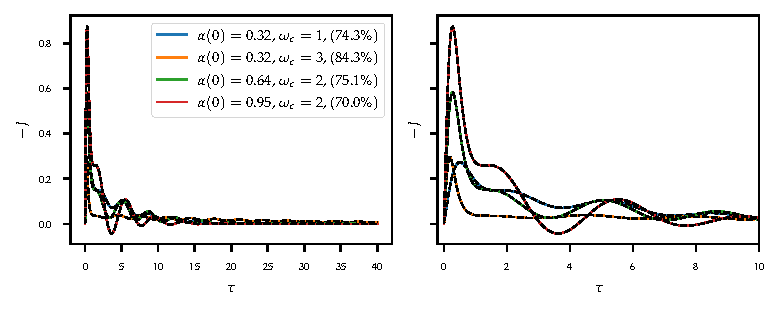
\includegraphics{figs/analytic_comp/flow_comp_zero.pdf}
  \caption{\label{fig:comp_zero_t} The bath energy flow \(-J\) for
    different parameters of the ohmic bath correlation function
    \cref{eq:ohmic_bcf}. The right panel shows the short time
    behaviour of the flow. The solid lines have been obtained with
    HOPS and the dashed lines using the analytic solution. A
    strikingly good agreement is evident visually and corroborated by
    the consistency values in parentheses the legend (see
    \cref{sec:meth} for an explanation).  The simulation with
    \(ω_{c}=3\) (orange) stands out for its slow long term decay,
    whereas the same simulation with longer bath correlation time
    (blue) decays much slower initially but falls below its orange
    counterpart for longer times.}
\end{figure}

\paragraph{Zero Temperature}
The bath energy flow \(J=-∂_t\ev{H_\bath}\), from here on called
simply ``the flow'' or ``bath energy flow'', for the zero temperature
case is plotted in \cref{fig:comp_zero_t}. The numerical results
(solid lines) agree with the analytical solutions (dashed lines) to a
very good accuracy, validating the findings of \cref{chap:flow}. For
all parameter choices the consistency is well above one standard
deviation.


The simulation was run with a hierarchy depth of
\(\abs{\vb{k}} \leq 5\) (simplex truncation\footnote{see
  \cref{sec:hops_basics}}) and a BCF fit with \(7\) terms taken from
\cite{RichardDiss} which was also used in the analytical solution. The
harmonic oscillator Hilbert space was truncated to \(15\) dimensions
in the energy basis. As the initial state the first excited state of
the oscillator was chosen so that some nontrivial energy flow would
occur. A reasonable number of \(N=5000\) trajectories have been
computed and lead to a quite satisfactory statistical error that is
small enough to be invisible in \cref{fig:comp_zero_t}. The normalized
standard deviation of the bath energy flow follows the usual
one-over-square-root rule as is illustrated in
\cref{fig:sqrt_conv}. Even after just \(N=1000\) trajectories the
normalized statistical error is on the order of \(10^{-3}\).
\begin{figure}[htp]
  \centering
  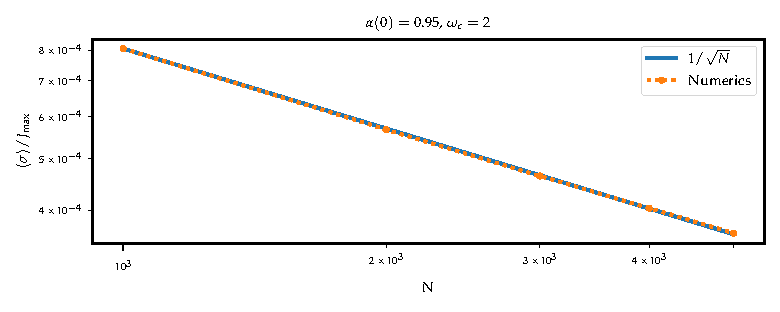
\includegraphics{figs/analytic_comp/sqrt_convergence.pdf}
  \caption{\label{fig:sqrt_conv} The (empirical) standard deviation
    (the statistical error) of the flow for the last configuration in
    \cref{fig:comp_zero_t} normalized by the maximum absolute value of
    \(J\). The \(1/\sqrt{N}\) rule is obeyed to good accuracy showing
    that the estimation of the variance is sound.}
\end{figure}
\begin{figure}[htp]
  \centering
  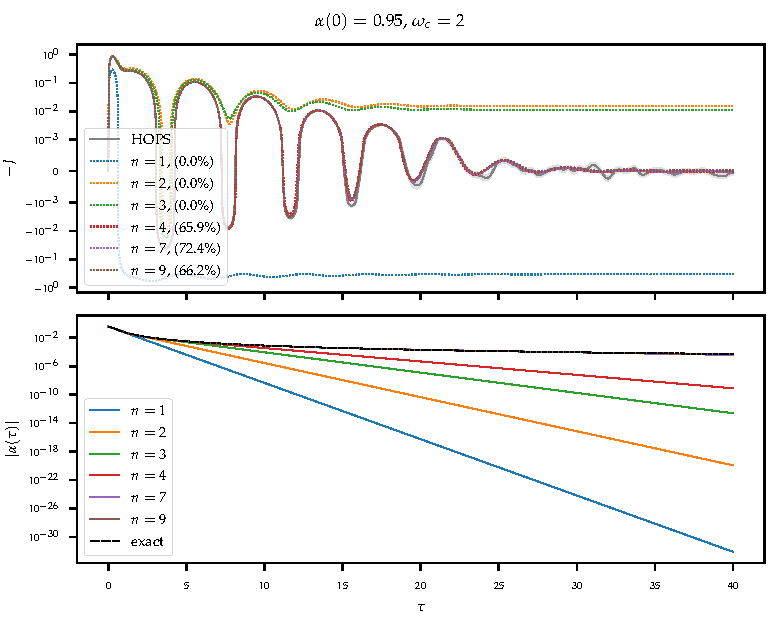
\includegraphics{figs/analytic_comp/analytical_terms_important.pdf}
  \caption{\label{fig:analytical_terms_important} Upper Panel: The
    analytical solution for the zero temperature bath energy flow
    using different numbers of terms in the BCF expansion in a
    symmetric logarithmic scale. For \(7\) terms the consistency
    (number in parentheses) with the numerical solution is best. For
    \(n<4\) the results are unphysical in the steady state.  Lower
    Panel: The absolute value of the approximated bath correlation
    function.}
\end{figure}

The analytical solution is quite sensitive to the quality of the BCF
expansion.  Despite choosing the same number of terms in the expansion
as in HOPS the simulation, there still remains a systematic difference
between HOPS and the analytical solution, as the stochastic processes
is sampled using the full bath correlation~\cite{RichardDiss}.
Nevertheless, the best agreement is found for using the same number
expansion terms in both HOPS and the analytical solution as is
illustrated in \cref{fig:analytical_terms_important}. Note that the
consistency value given in \cref{fig:analytical_terms_important} is
slightly different from the one in \cref{fig:comp_zero_t}, as here a
separate fit was made rather than using the fit from
\cite{RichardDiss}.

Interestingly, the solutions using a BCF expansion with three terms or
fewer lead to an unphysical non-zero steady state bath energy
flow. Considering specifically the case of one expansion term, this
may be related to the fact that now the corresponding spectral density
of \(α(τ)=G \exp(-Wτ)\) also has a finite value for negative
frequencies and will have negative parts when \(\Im G \neq 0\), making
it unphysical.  In general, the fit must model the decay of the BCF on
the appropriate time scales, to correctly reproduce the steady state.

Although the simulations are primarily intended as a benchmark for
HOPS and a verification for the results of \cref{chap:flow} some
observations can be made in \cref{fig:comp_zero_t}.

First, the flows for different parameters all feature the
characteristic spike in the flow, not unlike the phenomenon known and
discussed in the literature as ``initial
slip''~\cite{ChengMarkovianApproximationRelaxation2005,GaspardSlippageInitialConditions1999,HaakeAdiabaticDragInitial1983,SuarezMemoryEffectsRelaxation1992,YuPostMarkovMasterEquation2000}. As
the initial state is a product state which is unaware of the
bath-system interaction, the state undergoes some short time dynamics
to compensate the change of the effective oscillator dynamics due to
the interactions~\cite{Weiss2012}.% As we shall see in
% \cref{sec:one_bath_cutoff}, the interaction energy is generally
% negative. The surge in bath energy and also the system energy (see
% \cref{fig:ho_zero_entropy}) compensates for this. We will find in
% \cref{sec:moder-init-slip} that this effect can be compensated, by
% activating the interaction in a more adiabatic way.

We will discuss this phenomenon further in \cref{sec:pure_deph} as it
is a quite universal feature and also shows up on a single trajectory
level, suggesting that it is not strictly related to an energy
exchange with the bath but rather to the build-up of interaction
energy. This will be discussed further in \cref{sec:one_bath_cutoff}.

Note that the model of \cref{sec:oneosc} used here is missing a
so-called counter term, which is often prescribed to obtain a stokes
like, velocity dependent friction term in the equations of motion and
takes the form \cite{Weiss2008Mar}
\begin{equation}
  \label{eq:counter_term}
  H_{\mathrm{C}} \sim ∑_{λ}\frac{\abs{g_{λ}}^{2}}{ω_{λ}} q^{2}.
\end{equation}
When \cref{eq:counter_term} is included in \cref{sec:oneosc}, our
model becomes the Caldeira-Leggett Model~\cite{Caldeira1981Jan}.  In
many cases, the counter term balances the renormalization of the
system potential due to the bath. It is therefore an interesting
question how the initial slip behaves in its presence.

The time dependence of the flow also varies both with the shape of the
BCF and the coupling strength. For longer correlation times
\(τ_{\bath}\propto 1/ω_c\) we find that the flow initially decays much
slower at the same coupling strength (blue and orange lines) and
exhibits stronger oscillations. After this initial period the
situation is reversed and the simulation cuttoff frequency \(ω_{c}=3\)
(orange line) exhibits prolonged oscillations. For large coupling
strengths we can observe a ``backflow'' of energy out of the bath as
can be observed for the red line in the right panel of
\cref{fig:comp_zero_t}. In all cases the flow features some
oscillations and decays to zero which is physically reasonable for the
situation of a harmonic oscillator that loses most of its energy into
a zero temperature bath.

When the bath memory is short however, the short-term energy flow is
of less magnitude. Correspondingly, the system energy decays slower
for shorter bath memories \cref{fig:ho_zero_entropy}. We will discuss
this point further in \cref{sec:one_bath_cutoff} in the context of
another model as the performance does not only depend on the bath
memory, but also on the concrete distribution of the spectral density
in frequency space.

\begin{figure}[htp]
  \centering
  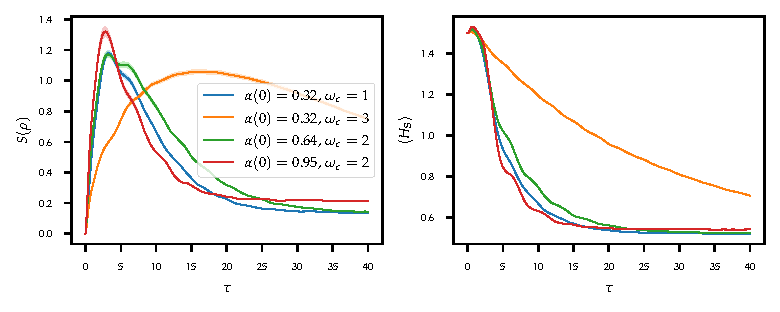
\includegraphics{figs/analytic_comp/entropy_zero.pdf}
  \caption{\label{fig:ho_zero_entropy} Left panel: The von Neumann
    entropy of the system state as a measure for entanglement with the
    bath. Right panel: The system energy as a function of time. The
    \(ω_{c}=3\) case (orange) is markedly different from the others,
    with a much slower decay of the system energy and slower entropy
    dynamics. The strongest coupling simulation (red) converges to a
    markedly different steady state.}
\end{figure}
The ``backflow'' of energy out of the bath observed in
\cref{fig:comp_zero_t} for stronger coupling seems to diminish the
advantage of stronger coupling over larger bath memories when it comes
to reducing the system energy. The decay of the system energy of the
model with the largest coupling strength \(α(0)\) (red curve) in the
right panel of \cref{fig:ho_zero_entropy} is barely faster than the
decay of the energy of the more weakly coupled model with longer
memory (blue curve), despite much larger coupling. Here backflow is
observed for stronger coupling which shortens the timescale of the
energy exchange. In \cref{sec:one_bath_cutoff} we will see, that this
phenomenon generically occurs for long bath memories in combination
with stronger coupling and learn how they might be exploited.

Note also, that the steady state is not a product state as can be
determined from the residual entropy in \cref{fig:ho_zero_entropy} for
the cases where the steady state has been approximately
reached\footnote{Note that the global state is pure, so that the
  system state entropy is the correct measure of entanglement}. The
stronger the coupling, the larger the entanglement of system and bath
as measured by the system entropy. The simulation with coupling
strength \(α(0)=0.95\) (red line) appears to be leading to a
qualitatively different steady state than the one with the same cutoff
but weaker coupling strength (green line). This also manifests in a
higher expected system energy in the steady state.

\begin{figure}[htp]
  \centering
  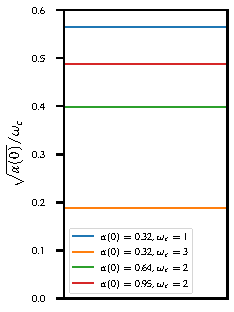
\includegraphics{figs/analytic_comp/timescale_comparison}
  \caption{\label{fig:timescale_comp} A comparison of bath vs
    interaction time scales
    \(\sqrt{α(0)}/ω_{c}\sim τ_{\bath}/τ_{\inter}\) for the simulations
    in \cref{fig:ho_zero_entropy}. The orange line is set far apart
    from the other simulations.}
\end{figure}
The time dependence of the system entropy and the system energy
expectation value is markedly different for the cutoff \(ω_c=3\)
(orange line). Although the coupling strength is similar to the
\(α(0)=0.32,\, ω_c=1\) case (blue line) the energy loss of the system
is much slower and the initial energy gain is less pronounced. This is
consistent with the flow in \cref{fig:comp_zero_t} which has a smaller
overall magnitude. The case is set apart by the long interaction
timescale \(τ_{\inter}\) due to the weaker coupling strength
\(\sim α(0)^{-1/2}\) and the short bath timescale
\(τ_{\bath}\sim ω_{c}^{-1}\). Of course absolute values of these time
scales are of no great value here. A comparison of relative time
scales \(\sqrt{α(0)}/ω_{c}\sim τ_{\bath}/τ_{\inter}\) can be found in
\cref{fig:timescale_comp} supporting the above argument.

\paragraph{Finite Temperature}
\begin{figure}[t]
  \centering
  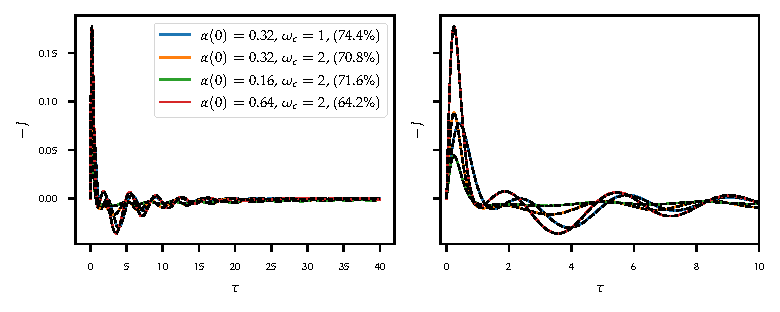
\includegraphics{figs/analytic_comp/flow_comp_nonzero.pdf}
  \caption{\label{fig:comp_finite_t} The bath energy flow \(-J\) of
    the quantum Brownian motion model for different parameters of the
    ohmic bath correlation function \cref{eq:ohmic_bcf} in the finite
    temperature \(T=1\) case. The presentation is equivalent to
    \cref{fig:comp_zero_t}.}
\end{figure}
The results for the finite temperature case are illustrated in
\cref{fig:comp_finite_t} for a temperature of \(T=1\). The setup was
otherwise equivalent to the zero temperature simulations, except for
the number of trajectories which was chosen to be \(N=10^5\) and the
initial state which was changed to the \(\ket{0}\) state.  Again the
high consistency values suggest that the findings of \cref{chap:flow}
are valid. The last case (\(α(0)=0.64,\, ω_c=2\), red line), falls
just short of the \(68\%\) mark, but agrees very well visually. It is
very probable that simply more samples are required.\fixme{maybe
  re-run...}

We find a similar behaviour to the zero temperature case, but this
time with a more pronounced flow (negative values in the plot) out of
the bath as it has a nonzero energy expectation value. For higher
coupling strengths, the flow amplitude is higher, as is also the case
for lower cutoffs.

One potentially contestable point in \cref{chap:flow} was the
appearance of the time derivative of the thermal stochastic process in
\cref{eq:pureagain}. The numerical method which is used to sample the
stochastic processes allows for a straight forward implementation of
this derivative so that no numerical derivatives are required and
there appears to be no problem.

As the dimensionality of the Monte Carlo integral underlying the
NMQSD/HOPS formalism is increased by the ``Stochastic Hamiltonian''
method, we observe markedly slower convergence as the variance of the
individual trajectories is higher. In \cref{fig:cons_dev_finite} the
convergence behaviour, as well the consistency with increasing
trajectory count are plotted and this symptom is observed. We also
find that in the more challenging regimes of stronger coupling or
longer bath correlation times the behaviour of the convergence is more
volatile, dipping into regions of inconsistency even at high sample
counts. While the mean difference between the numerical and the
analytical flow is always below the mean statistical error, larger
fluctuations can occur at certain points in time when a new region of
the probability space is sampled.

\begin{figure}[p]
  \centering
  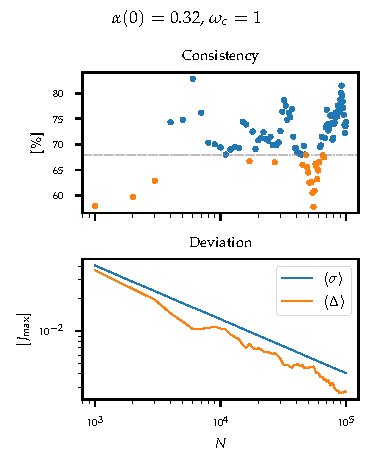
\includegraphics{figs/analytic_comp/consistency_development_0.pdf}
  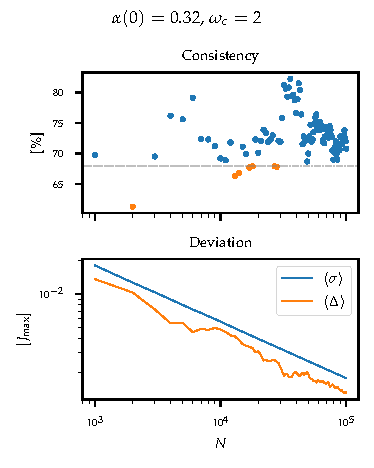
\includegraphics{figs/analytic_comp/consistency_development_1.pdf}
  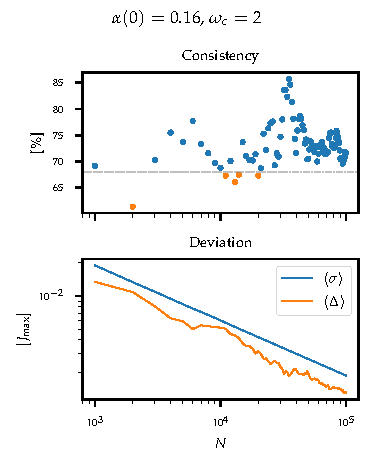
\includegraphics{figs/analytic_comp/consistency_development_2.pdf}
  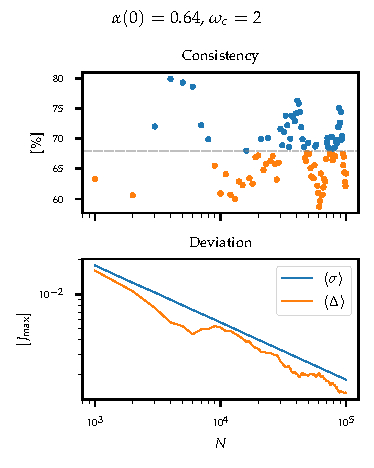
\includegraphics{figs/analytic_comp/consistency_development_3.pdf}
  \caption{\label{fig:cons_dev_finite} The convergence of the flows of
    \cref{fig:comp_finite_t} with increasing trajectory count. The
    upper panels show the consistency, where the grey line marks the
    \(68\%\) threshold for consistency. The lower panel shows the time
    averaged values of the statistical error \(\ev{σ}\) and the
    deviation from the analytical result \(\ev{Δ}\) normalized by the
    maximum absolute value \(J_{\mathrm{max}}\) of \(J\). In the last plot,
    the consistency development is quite unstable despite the mean
    deviation from the analytical result being smaller than the mean
    standard deviation. In all cases these two curves scale with the
    \(1/\sqrt{N}\) rule.}
\end{figure}

We have found, that we can expect precise numerical results for the
flow in the single bath case, both for zero and for finite
temperature. As systems with multiple baths are a different caliber,
both on the conceptual level, but also in the implementation of HOPS,
the method should also be verified for such settings. This will be
done in \cref{sec:twoosccomp}.
% The advantage of the ``Stochastic Hamiltonian'' method for finite
% temperature (see \cref{eq:thermalh}) is that one doesn't have to deal
% with the finite temperature BCF that does decay markedly slower than
% its zero temperature counterpart as is illustrated in
% \cref{fig:bcf_decay}. Generically, more terms in the BCF expansion
% would be required to capture the algebraic decay appropriately.

% \begin{figure}[t]
%   \centering
%   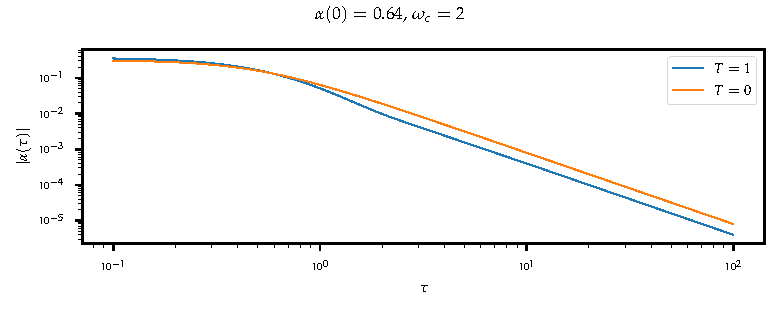
\includegraphics{figs/analytic_comp/bcf_decay.pdf}
%   \caption{\label{fig:bcf_decay} The absolute value of the Ohmic BCF
%     used in the last simulation of \cref{fig:comp_zero_t}.}
% \end{figure}

\subsection{Two coupled Harmonic Oscillators coupled to two Baths}
\label{sec:twoosccomp}
We now progress to a slightly more complicated setting, namely that of
two oscillators coupled to two baths\footnote{This also constitutes
  the first application of the TU-Dresden TQO group's HOPS code-base
  to multiple baths.}. As noted before, multiple baths are an
important ingredient for interesting models like quantum-thermodynamic
engines. At the same time, this setting is much more numerically
challenging as the number in BCF expansion terms doubles, which in
turn increases the number of hierarchy states.

The model of \cref{sec:oneosc} was generalized to two oscillators
coupled to two separate baths in \cref{sec:twoosc} and
\cref{eq:hamiltonian_two_bath}. In this section we simulate this model
and compare the results with the analytical solution.

For simplicity, the parameters were chosen symmetric so that the
frequencies of both oscillators are the same \(Ω=Λ=1\). As before,
\(Ω\) defines the energy unit. The zero temperature bath correlation
functions of both baths were identical with a cutoff frequency
\(ω_c=2\) and the intra-oscillator coupling was set to \(γ=0.5\). The
hierarchy was truncated so that \(\abs{\vb{k}}\leq 3\) and a BCF
expansion with five terms was employed to limit memory demands.  For
adequate convergence \(10^{4}\) trajectories were integrated.

To limit the variance, the temperature of one of the baths was set to
zero, so that only one thermal stochastic process was introduced.  The
other bath was initialized with the temperature \(T=0.6\) and the
initial state of the oscillators was chosen to be the ground state of
the system Hamiltonian \(\ket{0}\otimes \ket{0}\).

The main challenge of simulating the model
\cref{eq:hamiltonian_two_bath} is the dimension of the system Hilbert
space which is constrained by the available memory. In the simulation
discussed here, each oscillator was truncated at \(9\) levels leading
to a Hilbert space dimension of \(9^2 = 81\) in total\footnote{This is
  a naive method of truncation, but sufficient for the purposes of
  this work.}. The effect of a too drastic truncation of the system
Hilbert space can be seen in \cref{fig:insufficient_levels}. At the
temperature chosen, the mean level occupation of a harmonic oscillator
is given by the Bose distribution
\begin{equation}
  \label{eq:harm_mean_occ}
  \ev{n} = \frac{1}{\eu^{Ωβ}-1} \approx 0.23 < 1.
\end{equation}
Nevertheless, quite more than two-levels are required per
oscillator. This may be due to a required minimal resolution of the
position operators occurring in the model
\cref{eq:hamiltonian_two_bath} which is formulated with position space
in mind.

The final result can be studied in \cref{fig:sufficient_levels}. We
find good, but not excellent agreement. Based on the results of
\cref{sec:oneosccomp} however, it can be argued that this result is
sufficient to corroborate the validity of the results of
\cref{sec:multibath}. With more computational effort\footnote{Mainly
  more BCF expansion terms.} and fine-tuning of parameters an even
better agreement between the analytical and the numerical results may
be achieved. Note that the consistency figure given for the hot bath
is higher, as the statistical error bounds are greater due to the
finite temperature. These increased error bounds allow for more
deviation.
\begin{figure}[htp]
  \centering
  \begin{subfigure}[t]{.49\linewidth}
    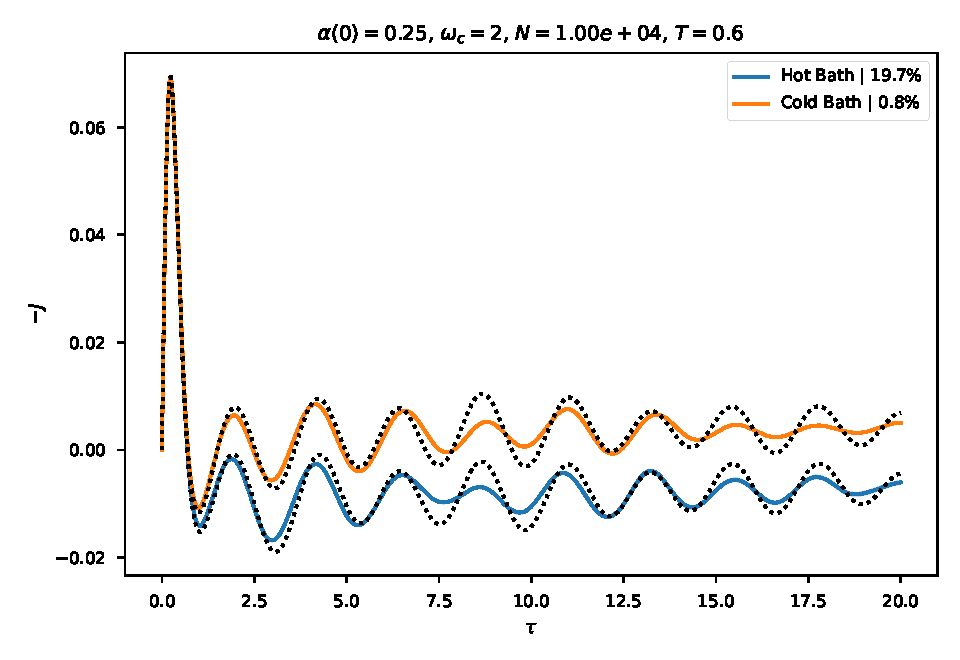
\includegraphics{figs/analytic_comp/comparison_two_5bcf_5ho.pdf}
    \caption{\label{fig:insufficient_levels}\(\dim\hilb_\sys=25\).  No
      agreement between the analytical solution and HOPS.}
  \end{subfigure}
  \begin{subfigure}[t]{.49\linewidth}
    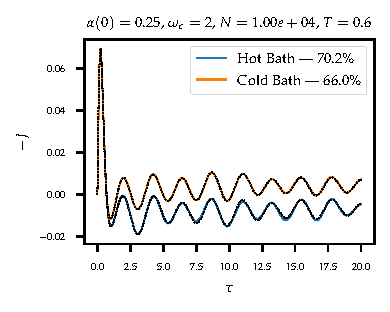
\includegraphics{figs/analytic_comp/comparison_two_ho.pdf}
    \caption{\label{fig:sufficient_levels}\(\dim\hilb_\sys=81\).}
  \end{subfigure}
  \caption{\label{fig:comp_two_bath} The bath energy flows for
    the model \cref{eq:hamiltonian_two_bath}, where the dashed lines
    correspond to the analytical solutions.}
\end{figure}

\Cref{fig:comp_two_bath} exhibits some interesting features. The
initial slip peak in the bath energy flows is identical for both baths
and independent of temperature as suggested by the discussion in
\cref{sec:pure_deph}. As is expected, the hot bath looses energy and
the cold bath gains energy, while this process is modulated by the
intra-oscillator coupling. It follows from the analytical solution
that eventually a steady state without oscillations will be reached.

The zero temperature bath flow converges very much faster than the
finite temperature flow despite the whole system being connected, at
least indirectly, to the hot bath. The reason for this is that the
derivative of the thermal stochastic process \(\dot{ξ}\) dominates the
variance of the flow for each trajectory. This is also the reason that
expressions depending on the hierarchy states rather than time
derivatives of stochastic processes are preferred as discussed in
\cref{sec:general_obs}.

We have shown that the findings of \cref{chap:flow} are consistent
with \cref{chap:analytsol} and that through a careful choice of the
HOPS parameters such as hierarchy depth, Hilbert space dimension and
BCF expansion the exact open system dynamics of the bath energy flow
can be reproduced. The statistical error can be made arbitrarily small
by increasing the trajectory count. For a given target error, the
required trajectory count can be estimated by the empirical standard
deviation of a given observable. In \cref{sec:pure_deph} we will
discuss the short term dynamics of our general model and explain the
peak in the flow, as seen in \cref{fig:comp_zero_t}.

For future work there remains the generalization of this section and
\cref{chap:analytsol} to time dependent couplings and
Hamiltonians. Because the NMQSD and also HOPS are largely agnostic of
these factors, we may safely assume that the results of the comparison
will be similar to the ones presented here.

Let us now turn to the short time behaviour of the flow and the
initial slip in \cref{sec:pure_deph} .

\section{Pure Dephasing and the Initial Slip}
\label{sec:pure_deph}
As evidenced in
\cref{fig:comp_finite_t,fig:comp_zero_t,fig:comp_two_bath}, the short
time behaviour of the bath energy flow is dominated by a
characteristic peak. Because this peak occurs at very short time
scales, it may in part be explained by a simple calculation which
neglects the system dynamics by setting \(H_\sys=0\).

We solve the model with the Hamiltonian (Schr\"odinger picture)
\begin{equation}
  \label{eq:puredeph}
  H = L^†(t) B + L(t) B^† + H_\bath
\end{equation}
with \(L(t)=L^†(t)\), \([L(t), L(s)] = 0\;\forall t,s\) (so that the
Heisenberg Hamiltonian matches \cref{eq:puredeph}) and \(B,\,H_\bath\)
as in \cref{sec:nmqsd_basics}.

Because \([L,H]=0\) we can immediately solve \(L_H(t)=L_S(t)\), where
the subscript distinguishes the Heisenberg and Schr\"odinger pictures
respectively. The Heisenberg equations for the \(a_λ\) yield
\begin{equation}
  \label{eq:alapuredeph}
  a_λ(t) = a_λ(0) \eu^{-\iu ω_λ  t} - \iu g_λ^\ast∫_0^t\dd{s} L(s)
  \eu^{-\iu ω_λ  (t-s)}.
\end{equation}

This allows us to calculate
\begin{equation}
  \label{eq:pureflow}
  \dot{H}_\bath =\iu\comm{H_{\inter}}{H_{\bath}} = - ∑_λ g_λ L(t) \qty[∂_t a_λ(0) \eu^{-\iu ω_λ t} - \iu
  g_λ^\ast∫_0^t\dd{s} L(s) ∂_t \eu^{-\iu ω_λ (t-s)}] + \hc,
\end{equation}
which gives with a state of the form \(ρ=\ketbra{ψ} \otimes ρ_β\)
\begin{equation}
  \label{eq:pureflowexpectation}
  \ev{\dot{H}_\bath } = -2 ∫_0^t\dd{s}\ev{L(t)L(s)} \Im[\dot{α}(t-s)],
\end{equation}
where \(ρ_β\) is a Gibbs state of inverse temperature \(β\).
For time independent \(L\) this becomes
\begin{equation}
  \label{eq:pureflowtimeindep}
  \ev{\dot{H}_\bath } = -2 \ev{L^2} \Im[α(t)].
\end{equation}
Note that \(α\) is the zero temperature BCF.

The proportionality to the imaginary BCF \(α\) does explain the
initial peak in the bath energy flow. The imaginary part is zero for
\(t=0\) and then usually features a peak at rather short times
(assuming finite correlation times). For the Ohmic BCF used here and
plotted in \cref{fig:ohm_bcf_ex} this feature is very prominent.
\begin{figure}[htp]
  \centering
  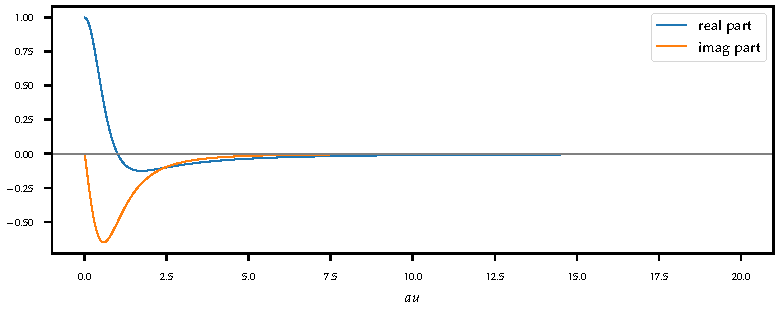
\includegraphics{figs/misc/ohmic_bcf_example.pdf}
  \caption{\label{fig:ohm_bcf_ex} An ohmic BCF with \(ω_{c}=η=1\). The
  imaginary part has a peak at the beginning and decays to zero.}
\end{figure}

Generically, the imaginary part of the BCF is negative at least for
short times as it takes the form
\begin{equation}
  \label{eq:negtive_imag}
  \Im[α(τ)] = -\frac{1}{π}∫_{0}^{∞}J(ω) \sin(ωτ)\dd{ω}
\end{equation}
which is negative for \(τ\leq π/ω_{\mathrm{max}}\), where
\(ω_{\mathrm{max}}\) is a characteristic cutoff frequency of the
system. The direction of the initial slip flow for unmodulated systems
will therefore always be into the bath compensating for negative
interaction energy.

Interestingly, \cref{eq:pureflowexpectation} does not contain any
reference to the temperature of the bath. Therefore, the bath energy
can only surpass its initial value in this model, as the dynamics
match the zero temperature case in which the bath has minimal energy
in the initial state.

A thermodynamically useful model should feature significant system
dynamics which is always given, assuming that the coupling is not too
strong. Non hermitian coupling may also have this effect, but in the
literature most effective two-level models tend to favour Hermitian
couplings
\cite{Aurell2019Apr,Hita-Perez2021Nov,Hita-Perez2021Aug,MacQuarrie2020Sep,Andersen2017Feb,Mezzacapo2014Jul}. For
the spin-boson model, non Hermitian coupling is the result of the
rotating wave approximation under the assumption that system and bath
time scales are quite different, which however does not imply weak
coupling~\cite{Irish2007Oct}.

For completeness, the interaction energy is given by
\begin{equation}
  \label{eq:pureinter}
  H_\inter = L(t)\qty[∑_λg_λ\qty(a_λ(0)\eu^{-\i ω_λ t} - \i
  g^\ast_λ∫_0^t\dd{s} L(s) \eu^{-\i ω_λ (t-s)})] + \hc,
\end{equation}
yielding
\begin{equation}
  \label{eq:pureinterexp}
  \ev{H_\inter} = 2 ∫_0^t\dd{s}\ev{L(t)L(s)} \Im[α(t-s)].
\end{equation}

For time independent coupling we have
\begin{equation}
  \label{eq:pureinterexp_timeidp}
  \ev{H_\inter} = 2 \ev{L^2} \int_{0}^{t}\Im[{α}(s)]\dd{s} = -Δ\ev{H_{\bath}}.
\end{equation}

It may be useful to normalize the BCF based on \cref{eq:pureinterexp},
so that the pure interaction energy build-up in the initial slip is
taken as measure of interaction strength. To make the normalization
independent of \(L(t)\), we choose the normalization to be
\begin{equation}
  \label{eq:bcfnorm}
  \begin{aligned}
  \mathcal{N} &= 2 \abs{\frac{\max_t\norm{L(t)L^\dag(t)+\hc}}{\max_t{\norm{H(t)}}} ∫_0^∞ \Im[α_u(τ)]\dd{τ}}\\
    α(τ) &= α_u(τ)/\mathcal{N},
  \end{aligned}
\end{equation}
where \(α_u\) is some unnormalized BCF. This normalization has the
useful property, that it neutralizes any scaling in \(L\). Note that
here the convention in which \(α\) is dimensionless is used.

% this is not true
% imaginary part becomes proportional to the Dirac delta in the limit
% where typical cutoff frequency \(ω_c\rightarrow ∞\). The integral over
% the real part of \(α\) always gives zero if the spectral density obeys
% \(J(0) = 0\) and tends to exhibit fast oscillations and fast decay in
% the large-cutoff limit. For weak coupling, it may therefore be
% neglected. This constitutes the Markov limit mentioned in
% \cite{Strunz2001Habil}.
The Ohmic-type BCF is
\begin{equation}
  \label{eq:normohmic}
  α(τ)=\frac{ω_c}{\max_t\norm{H} (1+\iu ω_c τ)^{2}},
\end{equation}
in this normalization.


This concludes the discussion, and we will move on to concentrate on
the numerical aspects and the phenomenology of the energy flow of the
spin-boson model in \cref{sec:prec_sim}.

\section{Precision Simulations of the Zero Temperature Spin-Boson Model}
\label{sec:prec_sim}
Despite being soluble analytically, the models from
\cref{sec:hopsvsanalyt} are numerically cumbersome, as their system
Hilbert space is infinite dimensional and has to be truncated. In this
section we concern ourselves with a very fundamental model that poses
lesser numerical challenges and still exhibits interesting
behaviour~\cite{RichardDiss,Link2022Feb}.

Both the performance of the HOPS method itself
(\cref{sec:stocproc,sec:trunc}) and the characteristics of the flow
mediated by the concrete form of the bath correlation function
(\cref{sec:one_bath_cutoff,sec:energy-transf-char,sec:one_bathcoup_strength})
will be investigated. We will find that the numerics do indeed yield
very consistent results and that the specifics of the energy flow
depend very much on the spectral density.

As an analytical solution to a given open system is generally not
known, another indicator of the proper choice of HOPS parameters is
required. Upon the example of a single qubit coupled to a single zero
temperature bath, we will study the precision of the HOPS method.  The
corresponding Hamiltonian is
\begin{equation}
  \label{eq:one_qubit_model}
  H = \frac{1}{2} σ_z + \frac{1}{2} ∑_λ\qty(g_λ σ_x^† a_λ + g_λ^\ast
  σ_x a_λ^†) + ∑_λ ω_λ a_λ^\dag a_λ,
\end{equation}
where we have chosen \(H\) to be dimensionless.

In the language of HOPS this corresponds to \(H_\sys=σ_z/2\),
\(L=σ_x/2\). We again choose the Ohmic BCF as explained in
\cref{sec:meth}. Throughout this section we choose the ``up'' state
\(H_S\ket{1} = 1/2\ket{1}\) as the initial state of the system.

The main measure of convergence for variables other than the
trajectory count are consistency conditions. One check available to us
is energy conservation, which allows us to calculate the expectation
value of the interaction energy through integration of the bath energy
flow. The interaction energy obtained in this way can then be compared
to the interaction energy obtained directly as shown in
\cref{sec:intener}. Note that this scheme may also be adapted easily
to multiple baths where the sum of interaction energies has to be
considered and to time dependent Hamiltonians where finite power has
to be taken into account.

Sources of systematic deviations for the model
\cref{eq:one_qubit_model} are the quality of the sampling of the
stochastic process and the truncation of the hierarchy. The first
becomes important when the cutoff frequency is large and the BCF
vanishes rapidly, necessitating a resolution of shorter time
scales. The hierarchy truncation is important when the cutoff
frequency is smaller and the bath has a longer memory.

\subsection{Stochastic Process}
\label{sec:stocproc}
For studying the convergence behaviour in reference to the sampling of
the stochastic process we chose the cutoff \(\abs{\vb{k}} \leq 4\)
(simplex truncation\footnote{see \cref{sec:hops_basics}}),
\(N=4.5 \cdot 10^5\) trajectories and an Ohmic BCF with \(α(0)=1.6\)
and \(ω_c=4\).  The sampling method uses the ``Fast Fourier
Transform'' (FFT) as described in \refcite{RichardDiss}. As the system
Hilbert space dimension is small, a BCF expansion with seven terms was
employed~\cite{Hartmann2021Aug,RichardDiss}.

The main parameter of this method is the accuracy of the FFT. The
implementation compares the BCF and its FFT approximation on the time
interval of the simulation to choose the internal
parameters\footnote{The number of time grid points and the integral
  boundaries in frequency space.} so that the difference of the FFT
transformed spectral density and the exact BCF normalized by \(α(0)\)
is smaller than a given value \(ς\).

\begin{figure}[htp]
  \centering
  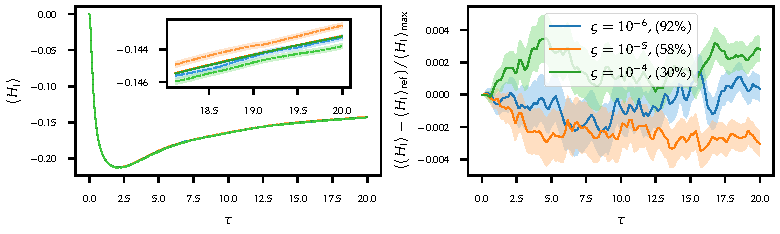
\includegraphics{figs/one_bath_syst/stocproc_systematics_interaction}
  \caption{\label{fig:stocproc_systematics} Left panel: The
    interaction energy of the model \cref{eq:one_qubit_model} for
    \(α(0)=1.6\) and \(ω_c=4\) using different precisions for the
    sampling of the stochastic process. The dashed lines are obtained
    using energy conservation while the solid lines are obtained
    directly through the use of \cref{sec:intener}. The consistency between
    the two is given in the legend of the right panel. An inset shows
    the curves for the final three time units. Right panel: The
    difference of the interaction energies obtained using energy
    conservation and directly. The values are normalized by the
    maximal absolute value of the interaction energy. The
    \(\varsigma = 10^{-6}\) case gives the most accurate results in
    terms of energy conservation, but when using the direct method of
    calculating \(\ev{H_{\inter}}\) all parameter choices yield the
    same results.}
\end{figure}
\Cref{fig:stocproc_systematics} illustrates the effect of this
parameter. We find very good qualitative agreement for all values of
\(ς\). The indirectly calculated values (dashed lines) of the
interaction energy exhibit some fluctuations between the settings, but
the directly calculated quantities (solid lines) are very stable as can
be witnessed in the inset of \Cref{fig:stocproc_systematics}.

Only in the simulation with precision \(\varsigma=10^{-6}\) (blue)
however, the compatibility condition of \cref{sec:meth} is satisfied
for the given trajectory count.  The system energy can be calculated
directly from the system state whereas the flow has to be integrated
numerically to obtain the total bath energy change and depends
directly on the first hierarchy states. The accuracy must be high for
the results to be consistent.
\begin{figure}[htp]
  \centering
  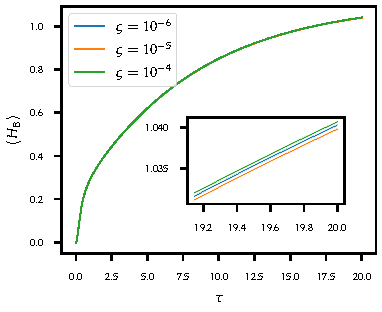
\includegraphics{figs/one_bath_syst/stocproc_systematics_bath_energy}
  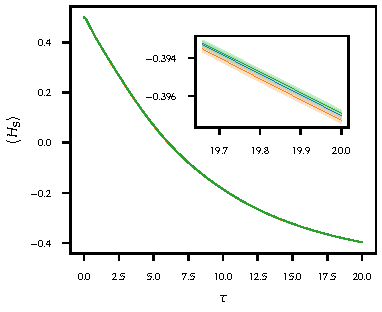
\includegraphics{figs/one_bath_syst/stocproc_systematics_system}
  \caption{\label{fig:stocproc_bath_sys}The bath and system energies of the
    model \cref{eq:one_qubit_model} for \(α(0)=1.6\) and \(ω_c=4\)
    using different precisions \(\varsigma\) for the sampling of the
    stochastic process. Systematic deviations outside the error bounds
  occur mainly in the bath energy.}
\end{figure}

The individual contributions to the indirectly obtained interaction
energy may be studied in \cref{fig:stocproc_bath_sys}. The bath energy
\(\ev{H_{\bath}}\), being an integrated quantity for which errors
accumulate, is most susceptible to systematic deviations outside the
error bounds, as is clearly visible in the insets. Nevertheless, the
qualitative agreement of the different simulations is excellent.

The development of the consistency over the trajectory count \(N\) is
plotted in \cref{fig:stocproc_consistency_dev}. Only for the highest
precision (blue) case good consistency is given continually. For lower
precision (green, orange), the consistency fluctuates and only
occasionally surpasses \(68\%\). Initially compatibility is being
demonstrated (until about \(N=10^4\)) but a divergence from
the most precise result occurs. It is therefore important to consider
the dependence of the compatibility on the sample count \(N\) to judge
the veracity of the simulation results.
\begin{figure}[htp]
  \centering
  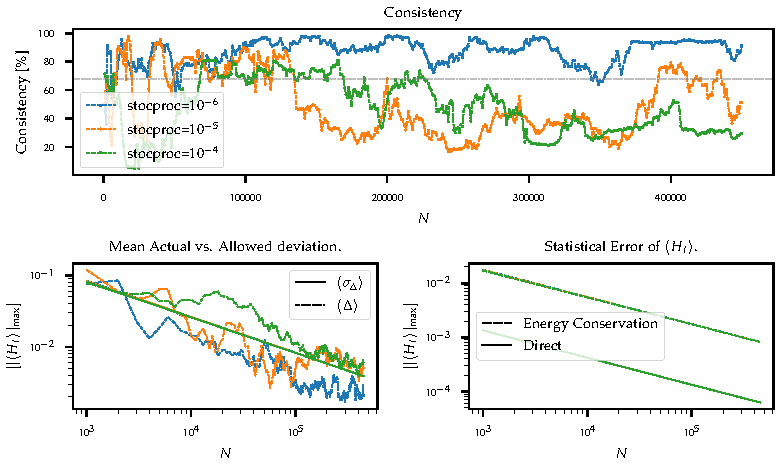
\includegraphics{figs/one_bath_syst/stocproc_systematics_consistency}
  \caption{\label{fig:stocproc_consistency_dev} Upper panel: The
    compatibility (number of values within one standard deviation of
    other, see \cref{sec:meth}) of the flow (direct computation
    vs. energy conservation) of the model \cref{eq:one_qubit_model}
    for \(α(0)=1.6\) and \(ω_c=4\) using different precisions
    \(\varsigma\) for the sampling of the stochastic process in
    relation to the trajectory count \(N\). Only the
    \(\varsigma=10^{-6}\) simulation is consistent for all sample
    counts. Lower left: The time averaged difference of the direct and
    indirect interaction energies (dashed) and the time averaged
    standard deviation of the difference (solid) as a function of
    trajectory count. Only for the smallest \(\varsigma\) the
    difference is consistently smaller than the standard deviation of
    the difference. Lower right: The time averaged statistical errors
    of the interaction energy calculated directly (solid lines) and
    indirectly through energy conservation (dashed lines). The
    deviation of the direct method smaller by an order of magnitude.}
\end{figure}

Apart from being closer to the correct result, the direct computation
of the interaction energy has the advantage of providing faster
convergence as is also demonstrated in
\cref{fig:stocproc_consistency_dev} (lower right panel).

\subsection{Hierarchy Truncation}
\label{sec:trunc}
As the systematics of the truncation depth have already been studied
thoroughly in \refcite{RichardDiss,Hartmann2021Aug}, we will keep the
discussion short.  We chose \(N=4.5 \cdot 10^5\) trajectories and an
Ohmic BCF with \(α(0)=0.8\) and \(ω_c=2\). Again, a BCF expansion with
seven terms has been used. The coupling strength has been chosen with
the help of \cref{sec:pure_deph}, so that the interaction energy is of
a similar order of magnitude as in the discussion above. The
simulation was run with \(k=\abs{\vb{k}}=∑_{i}k_{i}=\in \{2,4,6\}\).

\Cref{fig:k_systematics} suggests that there is to be no improvement
in accuracy or even change in the value of the flow for
\(k\geq 4\). However, the inset in the left panel
demonstrates that the direct result differs slightly for
\(k = 2\), which demonstrates that an adequate choice of
truncation depth is important.
\begin{figure}[htp]
  \centering
  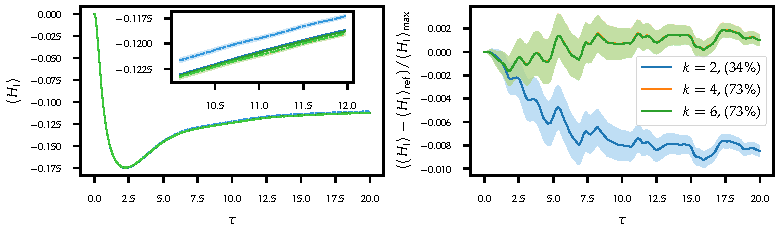
\includegraphics{figs/one_bath_syst/k_systematics_interaction}
  \caption{\label{fig:k_systematics} The same as
    \cref{fig:stocproc_systematics} but for \(α(0)=0.8\) and
    \(ω_c=2\) and for various truncation depths \(k=\abs{\vb{k}}_{\mathrm{max}}\).}
\end{figure}

We see in \cref{fig:k_systematics_system} that the difference of the
\(k = 2\) (blue lines) and the \(k = 6\) is on the same order of
magnitude for system energy (solid line) and interaction energy
(dashed line). The bath energy (dotted line), being an integrated
quantity, accumulates errors and deviates the most. Also, the results
for \(k = 4,6\) (orange line) appear to agree perfectly in all cases.
\begin{figure}[htp]
  \centering
  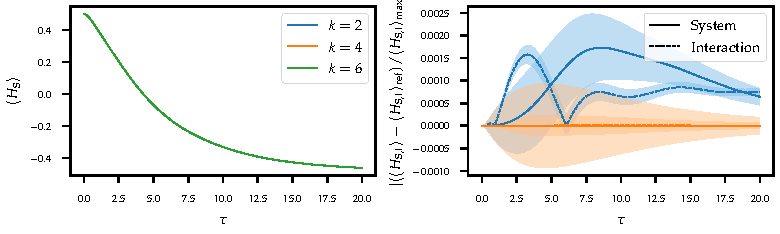
\includegraphics{figs/one_bath_syst/k_systematics_system}
  \caption{\label{fig:k_systematics_system} Legends: The legend in the
    left panel applies to both panels, whereas the legend in the right
    panel only applies to the right panel.  Left panel: The norm of the
    difference of a single trajectory to the \(k = 6\)
    case. The solid lines show the difference of the zeroth hierarchy
    states and the dashed lines show the same for the first hierarchy
    states.  There is still a slight difference on the trajectory
    level. Right panel: The difference between the \(k=6\) result and
    the results with \(k<6\) normalized by the maximal absolute system
    energy (solid lines) and the same for the interaction energy
    (dashed lines) as well as the bath energy change (dotted). The
    deviation is most substantial for the bath energy change, as
    errors can accumulate in the integration of the bath energy flow.}
\end{figure}
The left panel of \cref{fig:k_systematics_system} demonstrates, that
there is still a difference greater than the machine epsilon on the
level of the trajectories. This difference however, is small enough
not to impact observables much.

Summarizing, we conclude that the HOPS parameters have to be chosen
carefully for precision simulations, but that a more relaxed choice of
parameters already give a \emph{very} good qualitative picture
depending on the observable. Numerical integration should be avoided
where possible.

\fixme{maybe run a simulation with more hierarchy depth and more bcf
  terms, check whether there is a mistake} It remains for future work
to perform a detailed study of the systematics of the finite
temperature flow and modulated Hamiltonians. In the following sections
we will look at some examples of physically interesting settings with
less focus on the systematics.

\subsection{Varying the Cutoff Frequency}
\label{sec:one_bath_cutoff}
The lessons learned in \cref{sec:stocproc,sec:trunc} will now be
applied to simulate the spin-boson model \cref{eq:one_qubit_model}
with high consistency for various parameter choices of the cutoff
frequency \(ω_{c}\in\{1,2,3,4\}\) of the Ohminc BCF (see \cref{sec:meth})
\begin{equation}
  \label{eq:ohmic_bcf_repeat}
  α(τ) =
  \frac{η}{π}\qty(\frac{ω_c}{1+\iu ω_c τ})^2.
\end{equation}
Guided by these demonstrations, we'll turn to a more detailed analysis
of the role of non-Markovianity in the energy transfer characteristics
of the model. The quantification of the initial slip dynamics in
\cref{sec:pure_deph} will also be verified.

To make the interaction energies comparable to each other, the BCF
normalization of \cref{sec:pure_deph} is being used. Because of the
small size of the Hilbert space, we were able to choose a HOPS
configuration\footnote{\(\abs{\vb{k}}\leq 7\), seven BCF terms,
  \(\varsigma = 10^{-6}\)} that yields high-accuracy results, based on
the results of the previous section. The only problematic result is
the one for the cutoff \(ω_c=1\), but there is good qualitative
consistency in this case. The failing of the consistency check may be
due to insufficient time resolution, or simply because the bath memory
is so long, that the hierarchy depth was insufficient despite the
rather weak coupling. The normalized difference between the two
interaction energies for this simulation (blue line, right panel of
\cref{fig:omega_interaction_consistency}) is of the order of
\(10^{-3}\) and thus quite acceptable. The consistency test is a very
high bar to cross.
\begin{figure}[htp]
  \centering
  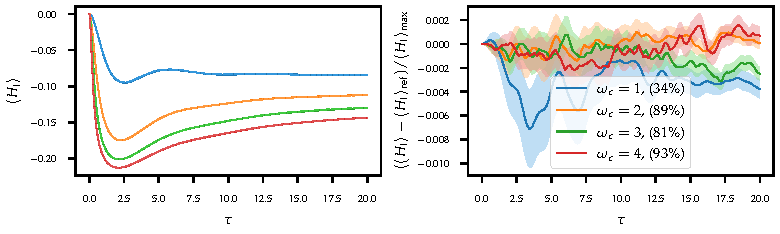
\includegraphics{figs/one_bath_syst/omega_interaction_consistency}
  \caption{\label{fig:omega_interaction_consistency}Interaction
    consistency plot for \cref{sec:one_bath_cutoff}, similar to
    \cref{fig:stocproc_systematics}. Good consistency is being
    achieved. The \(ω_{c}=1\) case (blue) does not pass the
    consistency test. Nevertheless, the qualitative agreement of the
    direct and indirect interaction energies (left panel) is quite
    good.}
\end{figure}

For all simulations \(N=5\cdot 10^{5}\) trajectories were integrated
to produce the results that are summarized in
\cref{fig:omega_systematics_system}.
\begin{figure}[htp]
  \centering
  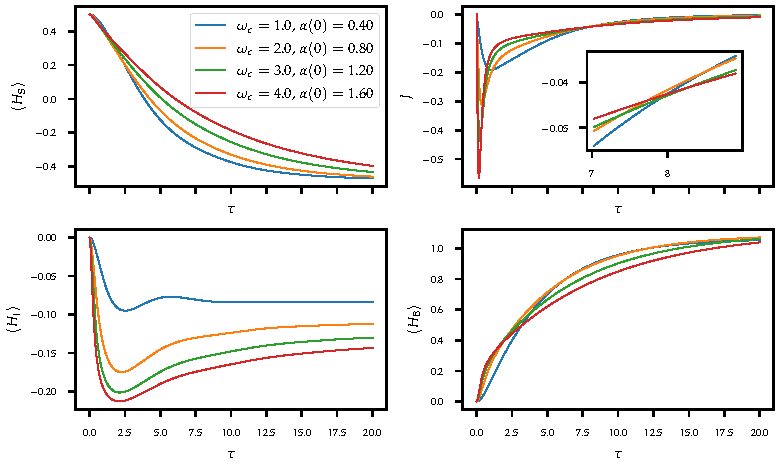
\includegraphics{figs/one_bath_syst/omega_energy_overview}
  \caption{\label{fig:omega_systematics_system} Energy overview for
    the spin-boson model \cref{eq:one_qubit_model} for various
    coupling strengths and cutoff frequencies. The curves are
    converged, and the error funnels are not visible. The \(ω_{c}=1\)
    stands apart from the others due to its long bath memory. The
    system energy loss is the fastest of all cases despite the weaker
    coupling as gauged by the magnitude of the interaction energy.}
\end{figure}
The interaction energy expectation values \(\ev{H_{\inter}}\)
(\cref{fig:omega_systematics_system}, upper left panel) differ
significantly, despite being roughly of the same order of magnitude
and not in the weak coupling regime. This illustrates the limitation
of the estimate in \cref{sec:pure_deph} and exemplifies the
nontriviality of the open system dynamics. Better estimates of the
interaction energy and thus interaction strength may be derived from
ideas similar to the ones discussed in \cref{sec:normest}.  Besides
their magnitude, the qualitative time dependence of the interaction
energies varies, especially between the configuration with the cuoff
frequency \(ω_c=1\) (blue) and the others.

The interaction energy curve of the simulation with the cutoff
frequency \(ω_c=1\) (blue) in \cref{fig:omega_systematics_system}
exhibits two pronounced turning points in contrast to the other
simulations. This behaviour is a symptom of the very long bath memory,
as we will discuss below. Further, despite having the weakest overall
coupling strength \(α(0)=0.4\), the system energy falls off the
fastest after a short period where it is above the other
configurations. This behaviour is also visible in the bath energy
expectation value, where this simulation almost reaches the same
levels as the \(ω_c=2\) configuration (orange) for \(τ\gtrsim 5\).

The flow \(J\) is generally negative (the bath gains energy) and
decays after an initial peak. All the flow graphs appear to be
crossing in about the same point \(τ\approx 7.7\) after which their
ordering by magnitude is reversed.  The inset shows that this isn't
precisely the case, nevertheless further investigation of this
phenomenon may of interest in the future.  Due to the pure dephasing
behaviour discussed in \cref{sec:pure_deph}, a greater cutoff coupled
with a greater coupling strengths leads to a higher peak in the flow
for short times. After the peak the flow decays the faster, the higher
the cutoff. The situation is reversed after some time.  This is due to
the fact that still more system energy is left to be transmitted to
the bath.

The presentation in \cref{fig:omega_systematics_system} is not
conducive to comparing the actual performance of the energy transfer,
due to the variable shape of the spectral density and the chosen
coupling strengths. Because the maximum of the Ohmic spectral density
is located at \(ω_c\), the special observed energy transfer behaviour
for \(ω_c=1\) is likely due to a resonance effect as the system energy
level spacing coincides with the maximum and the coupling is on the
weaker side.

The dissipator of the master equation for this two-level system only
depends on the value of the spectral density at the qubit level
spacing~\cite[p. 66]{Rivas2012}\footnote{There \(L=σ_{+}\), but this
  has no bearing on the connection to \(ω_{0}\).}  \(ω_{0}=1\), so
that it is reasonable to expect, that there may be variations whenever
its magnitude at this point changes.  On the other hand, a strong
dependence of the flow on the shape of the bath correlation function
beyond lamb-shift like influences is an indicator of the departure
from the weak coupling limit.  \fixme{Here, some master equation
  comparison would be nice.}

For these reasons, we now perform a more detailed analysis in
\cref{sec:energy-transf-char}.

\subsection{Energy Transfer Characteristics}
\label{sec:energy-transf-char}
After focusing on the systematics and achieving very high consistency
in our simulations, we continue to shed some light on the role of bath
memory and resonance between system and bath in the behaviour of the
energy transfer between system and bath.


For a systematic study of resonance, we first compare the flow for
frequency shifted ohmic spectral densities\footnote{See
  \cref{sec:shift_sp} for details.} with identical scaling \(α(0)\)
and cutoff frequency \(ω_c=2\). The shifted spectral density is given
by
\begin{equation}
  \label{eq:shift_sd}
  J_{\mathrm{s}}(ω_{s})= J(ω - ω_{s}),
\end{equation}
where \(ω_{s} > 0\).

\begin{figure}[htp]
  \centering
  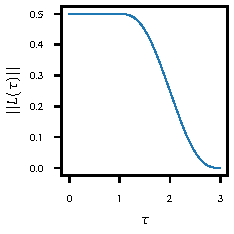
\includegraphics{figs/one_bath_syst/L_mod}
  \caption{\label{fig:L_mod} The smooth modulation of the coupling
    operator \(L(τ)\).}
\end{figure}
Also, we turn off the interaction smoothly\footnote{A smoothstep
  function of order two with a transition period of two. See
  \cref{sec:smoothstep}.} over two time units (see \cref{fig:L_mod})
before the system has reached its steady state and compare how much
energy has been transferred in terms of the final bath
\(\ev{H_{\bath}}\)\footnote{This is actually a slight misnomer, as we
  consider the \emph{change} of bath energy. The bath energy itself is
  infinite.} and system energies and the total energy change
\(Δ\ev{H}\) due to the modulated coupling.

This is the first time we make use of time dependent coupling. Despite
adding complexity to the method, this strategy simplifies our
discussion. Residual interaction energy is eliminated, making a
comparison of different simulations possible. Shifting the spectral
densities, another technical trick, allows us to study resonance
behaviour without altering the \emph{shape} of the spectral density,
again simplifying a comparison.

To make space for the shifted bath correlation functions in frequency
space, the qubit energy gap has been set to the value four so that
\(α(0)=8\) represents a quite reasonable coupling strength for the
purpose of studying energy transfer out of the system on a suitable
timescale.

We now define our measure of energy transfer performance.  The less
energy the system retains at the end of the protocol the better
performance of transfer. In other words, we want to transfer as much
energy out of the qubit as possible minimizing
\(\abs{\ev{H_{\sys}} + 2}\).  If the interaction energies
\(\ev{H_{\inter}}\) are on the same scale, the decoupling costs should
be roughly the same in terms of total energy change. Otherwise, they
may lead to an additional change of system and bath energies between
the different simulations.

Simulations for three values of the shift \(ω_{s}\in\{1,2,3\}\) are
being presented in \cref{fig:resonance_analysis}. For all shifts the
spectral density has a finite value at the value of system level
spacing, but only in the case with the cutoff \(ω_s=2\) (orange), the
resonance condition is fulfilled. Indeed, the energy transfer out of
the system \(\abs{\ev{H_{\sys}} + 2}\) is the best for the resonant
case (see \cref{fig:resonance_analysis}, middle panel), as the final
system energy is the lowest.

The change in total energy \(Δ\ev{H}\) (\cref{fig:resonance_analysis},
middle panel) due to the decoupling of the bath is moderately higher
in the resonant (orange) case than for cutoff \(ω_s=1\) (blue) and
seems to be somewhat proportional to the interaction energy, which is
reasonable. The decoupling process appears to affect mainly the bath
energy curves (dashed lines, left panel) in this case. Bath energies
\(\ev{H_{\bath}}\) generally decrease during decoupling, compensating
for the negative interaction energy. The effect on the system energy
is masked by the energy loss to the bath.

Were the interaction switched off abruptly, the system and bath
energies would remain untouched. Turning the interaction off in finite
time reduces the energy introduced into the system in the cases
discussed here. System and bath energy must therefore compensate part
of the negative interaction energy when the system is decoupled from
the bath. Hence, the observed lowering the bath energy after
decoupling. However the effect can also act into the other direction
as we shall see below.
\begin{figure}[htp]
  \centering
  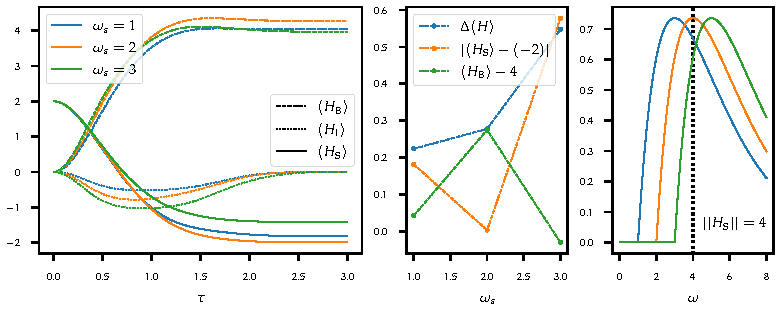
\includegraphics{figs/one_bath_syst/resonance_analysis}
  \caption{\label{fig:resonance_analysis} Left panel: The system, bath
    and interaction energies for various Ohmic BFCs with
    \(α(0)=8,\,ω_c=2\) shifted by \(ω_s\). Middle panel: The
    difference in total energy \(Δ\ev{H}\), the distance of the system
    energy to the ground state energy \(\abs{\ev{H_{\sys}} + 2}\) and
    the difference of the bath energy change and the initial system
    energy \(\ev{H_{\bath}} - 4\). Right panel: The spectral density
    for the three shift values \(ω_{s}\). \(\norm{H_\sys}\) does mean
    in this case, that the energy level spacing of the system is
    \(4\). The resonant case has the best energy transfer behaviour as
    gauged by the final system energy.}
\end{figure}

The third simulation with cutoff \(ω_s=3\) (green) exhibits the worst
energy transfer performance with the highest residual system energy
and the highest change in total energy due the large magnitude of the
interaction energy.  The lowering of the final bath energy is most
pronounced as the interaction energy is largest. As very much energy
is shed into to bath to build up the interaction, the bath energy
can't decay as much as in the simulation with cutoff \(ω_{s}=1\)
(blue).


Due to the asymmetry of the spectral density, the simulations for
\(ω_s=1\) and \(ω_s=3\) are not directly comparable. A repetition of
this investigation with a (pseudo) Lorentzian spectral density is left
to future work.

% Interestingly, also bath frequencies of \(ω_{0} + n Δ\) (\(n\in\NN\))
% become important if we modulate the system periodically with angular
% frequency \(Δ\), so that shifting the spectral density to higher
% frequencies is advantageous, albeit for the completely different
% objective of extracting energy from system and bath, as we will find
% out in \cref{sec:modcoup_reso}.

% Turning of the interaction leads mostly to a reduction of the final
% bath energy (see the middle panel).  This effect will also appear in
% most of the cases discussed below. When deriving a master equation for
% this two-level system~\cite[p. 68]{Rivas2012}, there occurs a lamb
% shift term that acts as a correction to the unitary evolution of the
% system. Turning the interaction off adiabatically removes this leads
% to a change in what one may define as system energy in this case. In
% the case discussed here, the coupling is not weak so that this
% explanation may only serve as a means of analogy. Compensating for the
% negative interaction energy, the system and bath energy expectation
% value both fall when the coupling is turned off.\fixme{is this
%   reasonable?}

% For an ohmic spectral density the lamb shift energy is
% \begin{equation}
%   \label{eq:lshift_twolevel}
%   2Δ=\eu^{-1/ω_{c}}\,\mathrm{Ei}\qty(\frac{1}{ω_{c}}) - ω_{c},
% \end{equation}
% which is negative for all the cases discussed here and may account for
% some part of the negative interaction energy. In this way, the removal
% of the bath would

\begin{figure}[htp]
  \centering
  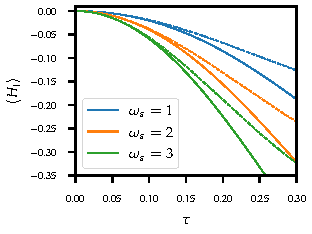
\includegraphics{figs/one_bath_syst/initial_slip_resonance}
  \caption{\label{fig:initial_slip_resonance} The interaction energies
    (solid lines) of the models in \cref{fig:resonance_analysis} and
    the predictions for the interaction energy due to the initial slip
    dynamics \cref{eq:pureinterexp_timeidp} (dashed lines). Larger
    frequency shifts of the spectral density lead to a higher
    magnitude of the interaction energy and faster dynamics.}
\end{figure}
As a heuristic observation, the maximal absolute interaction energy is
roughly proportional to the shift \(ω_{s}\) of the spectral density,
so that the short term interaction strength as measured by the
interaction energy expectation value is not only dependent on the
width and total norm of the spectral density, but also on its absolute
distribution in frequency space. The shift adds a phase factor
\(\eu^{-\i ω_{s} τ}\) to the BCF which makes the imaginary part
steeper for short times. This in turn leads to faster initial slip
dynamics and speeds up the buildup of interaction energy as
demonstrated in \cref{fig:initial_slip_resonance}. The observed effect
is sensible on an intuitive level as higher frequency oscillators are
being excited in the bath leading to faster dynamics.

Turning the interaction off later leads to the results of
\cref{fig:resonance_analysis_steady}. We see broadly similar energy
transfer characteristics for the cutoffs \(ω_{s}=1\) (solid blue line)
and \(ω_{s}=2\) (solid orange line).

For \(ω_{s}=3\) (green lines) the approximate steady state has not
been reached yet, and the energy transfer is incomplete so that the
residual system energy is the highest. As remarked earlier, the fast
growth of the interaction energy leads to a slower initial loss of
system energy. On longer time scales we see a slow, almost linear
transfer of energy from the system (solid line) into the interaction
(dotted line) as there is still is system energy left to be
transferred.
\begin{figure}[htp]
  \centering
  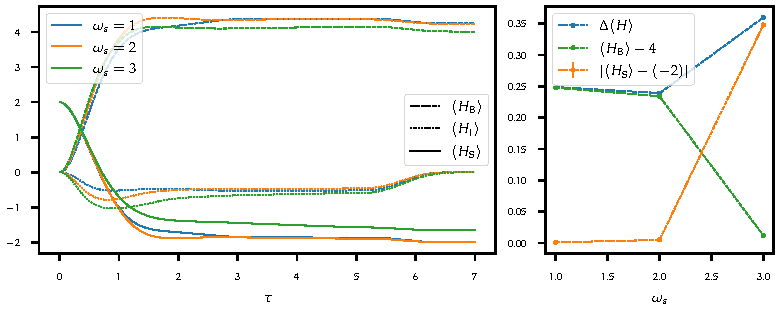
\includegraphics{figs/one_bath_syst/resonance_analysis_steady}
  \caption{\label{fig:resonance_analysis_steady} The same as
    \cref{fig:resonance_analysis} but for a longer coupling time.}
\end{figure}

Let us now turn to the impact of non-Markovianity on the energy
transfer into the bath.  To study the effect of the bath memory, we
use Ohmic spectral densities with linearly spaced
\(τ_{\bath}\equiv ω_c^{-1}\) that have been shifted and scaled by
numerical optimization so that their peaks coincide and the resulting
maximal absolute interaction energies are identical. This makes the
simulations more comparable, as otherwise very different energy
transfer speeds would be observed.

The rightmost panel of \Cref{fig:markov_analysis} shows plots of the
spectral densities obtained by the optimization. We can see, that not
only the magnitude at resonance point enters into the dynamics, as the
peak heights of the final spectral densities (right panel) are quite
different. We will encounter this behavior again in
\cref{sec:extr_mem}\footnote{Performing the optimization in the weak
  coupling regime will actually yield matching peak heights for the
  spectral densities.}.

The obtained results are very much dependent on the time when the
interaction is switched off. \Cref{fig:markov_analysis} has been
produced by tweaking the time point of decoupling so that an extremum
in the system energy of the long memory (\(τ_{B}=1\)) case (green) is
captured. This leads to an advantageous transfer performance with a
lower system energy and similar cost in terms of total energy change,
although residual system energy is still higher than in
\cref{fig:resonance_analysis_steady}.  Despite the system energy
initially fall off the fastest for the short memory case (blue) the
situation is reversed after about \(τ=0.5\).
\cref{fig:resonance_analysis_steady}.
\begin{figure}[htp]
  \centering
  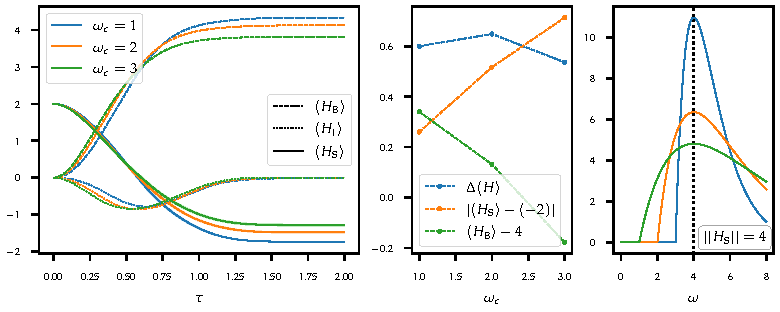
\includegraphics{figs/one_bath_syst/markov_analysis}
  \caption{\label{fig:markov_analysis} The same as
    \cref{fig:resonance_analysis} but for spectral densities of
    differing widths. The interaction was turned off smoothly over two
    time units beginning at \(τ=0\). The long-memory case performs
    best in this case, exhibiting the lowest final system energy. }
\end{figure}

Because the minimum in the interaction energy of the case with bath
memory \(τ_{\bath}=1\) (green) comes last, the residual interaction
energy and thus interaction strength is strongest when the interaction
is turned off smoothly beginning at \(τ=0\). Therefore, the largest
quantity of energy is being introduced into the system in this case
due to the modulation of the coupling. In all cases the amount of
energy introduced is so large, that the bath energy slightly rises
during the decoupling process instead of falling as in
\cref{fig:resonance_analysis_steady}.


\begin{figure}[htp]
  \centering
  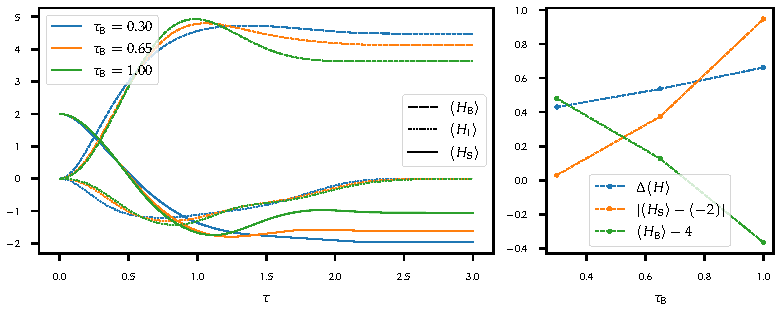
\includegraphics{figs/one_bath_syst/markov_analysis_longer}
  \caption{\label{fig:markov_analysis_longer} The same as
    \cref{fig:markov_analysis} but with slightly different timing.
    The interaction was turned off smoothly over two time units
    beginning at \(τ=1\). The result is exactly the reverse of
    \cref{fig:markov_analysis_longer}. Longer memories perform worse.}
\end{figure}
For slightly longer coupling times when the coupling is turned off
beginning at \(τ=1\) but with the same coupling strengths, we find in
the exact opposite picture as can be ascertained from
\Cref{fig:markov_analysis_longer}.  The increased bath memory time
allows for ``back flow'' of energy from the bath into the system (blue
and orange solid lines) and thus the performance of energy transfer is
strongly dependent on the precision of control. The oscillations of
flow and thus bath energy have already been noticed in
\cref{sec:oneosccomp} and seem to be a robust feature of stronger
coupling and long bath memories.

The total energy introduced is slightly less than in the earlier
simulation as the interaction energy is lower when the interaction is
switched off. The final bath energy shows an inverse behaviour,
falling as the final system energy rise. This is due to the similar
total energy change \(Δ\ev{H}\) in all three cases (blue line, right
panel). Similar correlations can also be observed in
\cref{fig:markov_analysis}.

For even longer times (the interaction was turned off smoothly
beginning at \(τ=18\)) we find in \cref{fig:markov_analysis_steady} a
picture similar to \cref{fig:markov_analysis_longer}. The short memory
case (blue) exhibits hardly any backflow and performs best in terms of
final system energy which is extremely close to the target value of
negative two. The other two bath memories perform worse (green,
orange). We observe that simulation with the longest bath memory
\(τ_{\bath}=1\) (green) stands out and having a very different final
state as is exemplified by the final system energy and the interaction
energy curve which exhibits a greater magnitude and persistent
oscillations. These oscillations were not clearly visible in the
earlier simulations
(\cref{fig:markov_analysis,fig:markov_analysis_longer}) due to the
modulation of the interaction. Because of the long memory, the bath,
interaction and, to a lesser extent, the system can continue to
exchange energy, even in the steady state. We will encounter them
again in a different setting in \cref{sec:extr_mem}.
\begin{figure}[htp]
  \centering
  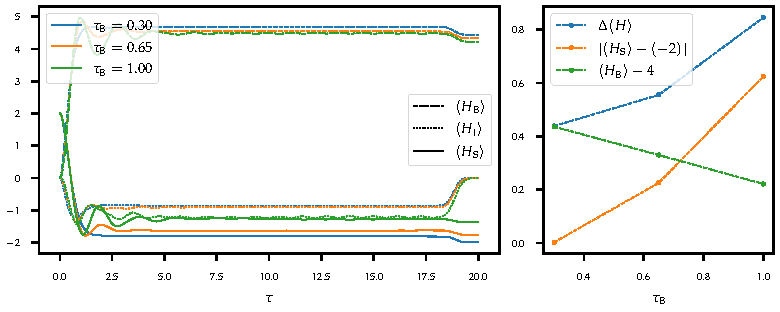
\includegraphics{figs/one_bath_syst/markov_analysis_steady}
  \caption{\label{fig:markov_analysis_steady} The same as
    \cref{fig:markov_analysis} but for long times.  The interaction was turned off smoothly over two
    time units beginning at \(τ=18\). The results are
    broadly similar to \cref{fig:markov_analysis_longer} with the
    \(τ_{\bath}=1\) case standing out.}
\end{figure}

In the two simulations with shorter memory (blue and orange lines) we
find that about half of the interaction energy is compensated by the
total energy change. The rest is accounted for by a lowering of system
and bath energy alike, an effect that is strongest in the short memory
\(τ_{\bath}\) case especially for the system energy. A slower, more
adiabatic coupling modulation could likely further reduce the amount
of energy introduced.

That the steady state system energies\footnote{Before the interaction
  is switched off.} are greater than the ground state energy of the
system in all simulations of \cref{fig:markov_analysis_steady} is a
token of strong coupling. The ground state of the two-level system is
not the steady state, as it would be in the weak coupling
limit~\cite{Binder2018}.

\paragraph{Non-Markovianity}
We have often alluded to the fact that oscillations in the system
energy, the back-flow of energy into the system, are a token of
departure from the Markovian regime. An explicit demonstration of this
fact is given in \cref{fig:steady_relent}.

Spohn's theorem~\cite{Breuer2002Jun} states that the negative time
derivative of the relative entropy of system state and steady state
must be positive if the dynamics are generated by a Markovian master
equation with a constant Hamiltonian.  In mathematical terms Spohn's
theorem can be formulated as
\begin{equation}
  \label{eq:spohn}
  -\dv{\qrelent{ρ_{\sys}(t)}{ρ_{\sys}(∞)}}{t} \geq 0,
\end{equation}
where \(\qrelent{ρ}{σ}=\tr[ρ \log_{2} ρ - ρ \log_{2} σ]\) is the
quantum relative entropy. The left-hand side of \cref{eq:spohn} is
often called entropy production~\cite{Breuer2002Jun,Binder2018}.
\begin{figure}[htp]
  \centering
  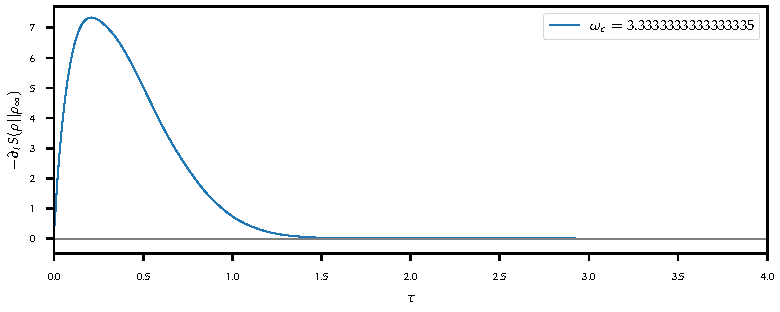
\includegraphics{figs/one_bath_syst/steady_relent}
  \caption{\label{fig:steady_relent} The negative time derivative of
    the relative entropy of system state and the approximate steady
    state (before the interaction is switched off) of the simulations shown in
    \cref{fig:markov_analysis_steady}. The short memory case does not
    violate Spohn's inequality, but the other two cases do.}
\end{figure}

\Cref{fig:steady_relent} demonstrates that the two simulations with
longer bath (green, orange) memories are inconsistent with Markovian
dynamics, as their entropy production exhibits strong negativity.

The enhanced short term energy transfer for long bath memories may be
understood qualitatively through the NMQSD equation.%   Let \(τ^{\ast}\)
% be the time in which the BCF decays sufficiently and \(τ\) be some
% point in time with \(τ>τ^{\ast}\). The NMQSD equation
% \cref{eq:nmqsd_single} features two terms that model the interaction
% with the bath. The driving term
% \begin{equation}
%   \label{eq:nmqsd_driving}
%   L {η}^\ast_t\ket{ψ({η}^\ast_t, t)}
% \end{equation}
% includes the bath memory in an indirect manner through the stochastic
% process \(η^\ast\). At the time point \(τ\), the process will be
% effectively uncorrelated with itself at \(τ-τ^\ast\). Increasing
% \(τ^\ast\) will make the fluctuations of \(η^\ast\) slower and reduce
% their magnitude as demonstrated in \cref{fig:stocproc_comparison}.
% This allows for steadier dynamics with a slower bath induced change in
% the trajectory and state.
% % This in turn reduces the fluctuations of the bath energy flow on a
% % trajectory level and allows for steadier accumulation.  This effect
% % may be best understood by looking at the alternative expression for
% % the flow \cref{eq:alternative}
% % \(\dot{η}_t^\ast \mel{\psi(η,t)}{L}{\psi(η^\ast,t)}\), which features
% % the derivative of this process directly.

% The memory term
% \begin{equation}
%   \label{eq:nmqsd_memory_term}
%   L^†∫_0^τ\dd{s}α(t-s)\fdv{\ket{ψ({η}^\ast_t, t)}}{η^\ast_s}
% \end{equation}
% contains the bath correlation time even more explicitly. One may
% choose the integration range in \cref{eq:nmqsd_memory_term} to be
% \((τ-τ^\ast, τ)\) in good approximation due to the decay of the
% BCF. Thus, the evolution of the trajectory is not being directly
% influenced by times before \(τ-τ^\ast\). Also, if the stochastic
% process fluctuates more slowly, the trajectory has a stronger
% dependence on its past values, enhancing the magnitude of the
% functional derivative.  We see therefore, that the memory time of the
% bath has a very direct influence on the dependence of the trajectory
% and therefore system dynamics on its earlier states.

The memory term
\begin{equation}
  \label{eq:nmqsd_memory_term}
  L^†∫_0^τ\dd{s}α(t-s)\fdv{\ket{ψ({η}^\ast_t, t)}}{η^\ast_s}
\end{equation}
creates an explicit dependence of the system dynamics on earlier
states and connects the bath memory encoded in the BCF \(α\) with the
actual dynamics. The longer the bath memory is, the smoother is the
stochastic process \(η_{t}^\ast\) and the greater is the influence of
the memory term. These facts can be observed in
\cref{fig:memory_term,fig:stocproc_comparison}, where it is clearly
visible that a greater bath memory time \(τ_{\bath}\) leads to a
greater influence of the memory term and smoother processes.
\begin{figure}[htp]
  \centering
  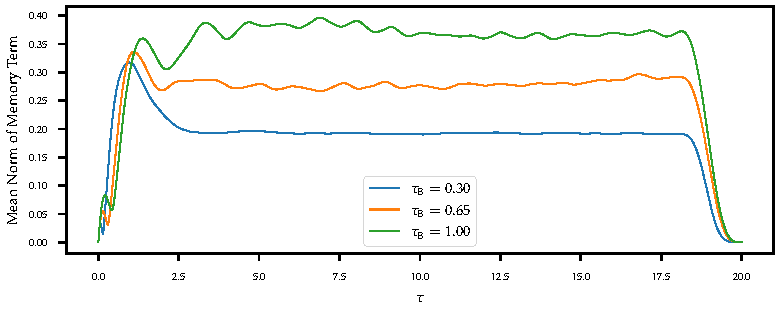
\includegraphics{figs/one_bath_syst/memory_term}
  \caption{\label{fig:memory_term} The norm of the memory term
    \cref{eq:nmqsd_memory_term} averaged over \(N=500\) trajectories
    from the simulations shown in
    \cref{fig:markov_analysis_steady}. The longer the bath memory
    \(τ_{\bath}\), the greater the influence of the memory term.}
\end{figure}

As the memory is mediated by the bath degrees of freedom, a dependence
on ever earlier system states must be due to ever longer interaction
with specific bath degrees of freedom which are independent themselves
except for their interaction with the system.

This interpretation is corroborated by a time discrete version of the
NMQSD discussed in \refcite{RichardDiss}. There, the
\emph{Time-Oscillator picture} is introduced, which shows that a
variant of the NMQSD can be formulated as the successive interaction
in time of the system with mode like degrees of freedom. At each time
step, a new oscillator is being coupled to the system and the coupling
to the existing oscillators is weakened according to the bath
correlation function.

With this in mind, we may conclude that because we interact for a
longer time with certain ``portions'' of the bath degrees of freedom,
the energy exchange between the bath and the system can be greatly
affected, as the energy exchange with the individual modes becomes
more complete.  At the same time, energy may flow back into the system
from those degrees of freedom if the bath memory is sufficiently
long.

In summary, we find that the energy dynamics of system, interaction
and bath depend strongly on the characteristics of the bath.  In the
regime studied, optimizing for fast energy loss of the system favours
longer bath memories, whereas the situation is reversed when longer
coupling times are allowed.

A resonance phenomenon has been observed which is already present in
the weak coupling case. However, here we additionally found a strong
dependence of the dynamics upon the shape of the whole spectral
density.

Note that the short time behaviour discussed here can usually not be
resolved by the usual Markovian master equations. This is due to the
fact, that the bath timescale \(\sim 1/ω_{c}\) must be by far the
shortest, which often isn't the case here. Another demonstration of
this fact is given in \refcite{Link2022Feb}, where Markovian dynamics are
compared with the Redfield and exact dynamics for the spin-boson model
coupled to a squeezed bath. As in \refcite{Xu2022Mar}, the Redfield
description is found to be adequate for weak coupling. This is due to
the Redfield master equation not requiring the secular approximation,
but only weak coupling. It can therefore faithfully capture
non-Markovian dynamics.

Let us now complete our precision studies of the zero temperature
spin-boson model energy flow by looking at the effect of different
coupling strengths in \cref{sec:one_bathcoup_strength}.

\subsection{Varying the Coupling Strength}%
\label{sec:one_bathcoup_strength}
\begin{figure}[htp]
  \centering
  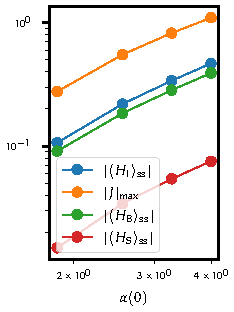
\includegraphics{figs/one_bath_syst/final_states_flows}
  \caption{\label{fig:delta_fs_flow} The absolute value difference of
    the state energies and the maximal flows for the simulations in
    \cref{fig:delta_energy_overview} from their value at coupling
    strength \(α(0)=0.40\) normalized by their value at
    \(α(0)=1.12\).}
\end{figure}
After having studied the dependence of the bath energy flow for
various cutoff frequencies of the BCF in \cref{sec:one_bath_cutoff},
we now consider the case with fixed cutoff \(ω_c=2\) but varying
coupling strength. The results presented here are mainly a
demonstration of the feasibility of high-consistency simulations for a
range of coupling strengths. We will therefore keep the discussion of
the physical implications relatively short.

The chosen simulation parameters are the same as in
\cref{sec:one_bath_cutoff} and again consistent results have been
obtained throughout the whole range of coupling
strengths.\footnote{see \cref{sec:intercons} for details} The
interaction strength was chosen linearly spaced, and the simulation
results are presented in \cref{fig:delta_energy_overview}.

As the shape of the BCF is not altered between the simulations, the
bath energy flow curves are of very similar shape, as are the
interaction energy curves. The main difference between the simulations
is the magnitude of the interaction energy. With increased coupling
strength there is an increased interaction energy and an increased
flow, which leads to faster energy loss in the system and faster
energy gain of the bath. The stronger the coupling becomes, the more
pronounced is the non-monotonicity in time of the interaction energy,
which is reflected in a non-monotonicity in the bath energy
expectation value.

The bath energy reaches a maximum and falls slightly for the strongest
coupling simulations (violet and brown lines). If the interaction is
strong enough, ``backflow'' can occur despite finite bath correlation
times. Here we can't witness any backflow of energy into the
system. The falling bath energy is likely an effect of energy
conservation. As the interaction energy rises after its initial
minimum, the bath energy falls to compensate in the strong coupling
cases.
\begin{figure}[htp]
  \centering
  \includegraphics{figs/one_bath_syst/δ_energy_overview}
  \caption{\label{fig:delta_energy_overview} Energy overview for the
    model \cref{eq:one_qubit_model} for various coupling
    strengths. The curves are converged out, and the error funnels are
    not visible.}
\end{figure}

As a task for future work it might be worthwhile to ascertain the
exact conditions under which system energy might flow back into the
system. Is resonance required and what role is played by the system
timescale? Does backflow always occur provided the coupling is strong
enough?\footnote{The author expects a negative answer to this
  question.}

Despite these differences for finite times, \cref{fig:delta_fs_flow}
demonstrates that the approximate steady state\footnote{excluding the
  \(α(0)=0.4\) case} interaction energies
\(\ev{H_{\inter}}_{\mathrm{ss}}\) (blue), maximal flows
\(\abs{J}_{\mathrm{max}}\) (orange), system energies
\(\ev{H_{\sys}}_{\mathrm{ss}}\) (red) and bath energies
\(\ev{H_{\bath}}_{\mathrm{ss}}\) (green) are almost linearly dependent
on the coupling strength \(α(0)\) in the range we studied.

We find that we can control the speed of the energy transfer between
bath and system with the coupling strength at the cost of greater
steady state interaction energy. Were we to turn off the interaction
diabatically, we would have to expend this energy in the worst
case. On the other hand, more adiabatic protocol as the one used in
\cref{sec:energy-transf-char} would likely be a remedy to this
drawback. In fact, the system energy is most likely lowered even
further when then interaction is turned off as we witnessed in
\cref{fig:markov_analysis_steady}.

Both the final system and bath energies are increasing with the
coupling strength, compensating for the interaction energy. This is
the main mechanism that leads to residual system energy in the steady
state which is further and further away from the ground state.

We discussed the short term dynamics for a general model in
\cref{sec:pure_deph}.  Now, in \cref{sec:initial-slip-sb} we will
study them in the case of the spin-boson model.

\fixme{iftime: re-run with same coupling strength, more cutoff freqs,
  less samples, see, longer times for coupling strengths, more coup}

\subsection{Initial Slip}%
\label{sec:initial-slip-sb}
\begin{figure}[htp]
  \centering
  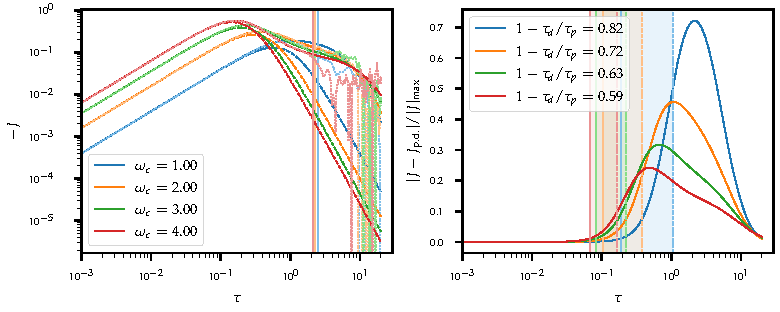
\includegraphics{figs/one_bath_syst/omega_initial_slip}
  \caption{\label{fig:omega_initial_slip} Left panel: The bath energy
    flow of the model \cref{eq:one_qubit_model} for various coupling
    strengths (solid lines) and the pure dephasing flow of
    \cref{sec:pure_deph} (dashed lines). The dotted lines show the
    flow calculated from one trajectory and the vertical lines mark
    the position of the peak of the absolute value of the interaction
    energy. Right panel: The difference of the actual flow \(J\) and
    the pure dephasing flow \(J_\mathrm{p.d.}\). The solid vertical
    lines mark the time \(τ_p\) where the normalized deviation from
    pure dephasing is \(10^{-2}\) and the dashed vertical lines show
    the position of the peak flow at time \(τ_p\). The divergence from
    pure dephasing dynamics occurs before the peak flow and the
    earlier the longer the bath memory is. The single trajectory flow
    matches the exact flow for a longer period.}
\end{figure}

As the initial peak in the energy flow is also very prominent in the
simulations in this chapter, we return to
\cref{fig:omega_systematics_system} and compare the dynamics of those
simulations to the pure dephasing case of \cref{sec:pure_deph}. A good
agreement for short times is to be expected, as the system can't take
up energy in its initial state (up), so that all of the interaction
energy must initially be compensated solely by the bath.

In \cref{fig:omega_initial_slip} we plotted a comparison of the exact
dynamics and the pure dephasing solution. The pure dephasing dynamics
(dashed lines) are accurate for the very short time scales, but fail
to predict the correct location of the peaks in the absolute value of
the exact bath energy flow (solid lines).  The deviation occurs before
the peak, where the time difference between the peak and the deviation
increases with increasing bath memory \(\propto 1/ω_c\), as does the
magnitude of the maximal deviation (right panel). This can be
ascertained from the legend of \cref{fig:omega_initial_slip} where the
difference between deviation and peak time normalized by peak time is
given.

We can conclude that for longer bath memory along with weaker
coupling, the role of the system Hamiltonian dynamics in modulating
the flow becomes increasingly important as the approximation
\(H_{\sys}\approx 0\) becomes increasingly invalid.

The flow calculated from a single trajectory (dotted lines in
\cref{fig:omega_initial_slip}) matches the exact flow longer than
the pure dephasing approximation. For large cutoffs \(ω_{c}\) (green
and red) the single trajectory even matches until after the peak flow,
whereas the deviation occurs earlier for the \(ω_{c}=1\) case
(blue). The stochastic nature of the single trajectory dynamics seems
to become important only after a finite amount of time, longer than
period of pure dephasing dynamics.

\begin{figure}[htp]
  \centering
  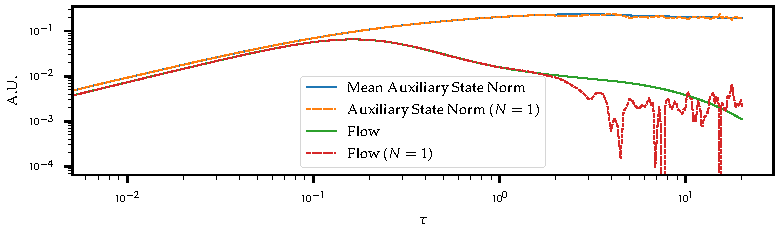
\includegraphics{figs/one_bath_syst/flow_buildup}
  \caption{\label{fig:flow_buildup} The norm of the auxiliary
    states of hierarchy depth one
    (\(\sqrt{∑_{i}\braket{ψ^{\vb{e}_{i}}}}\)) and the flow for
    one trajectory and as a mean over all trajectories for the
    \(ω_{c}=4\) simulation. For short times the results for one
    trajectory match the ensemble means. The divergence between one
    trajectory and the mean occurs at roughly the same time for the
    flow and the auxiliary state norm. Moreover, flow and mean
    auxiliary state norm have the same functional form for very short
    times, apart from a scaling factor. The initial dynamics are
    therefore mainly concerned with populating the auxiliary states.}
\end{figure}
For short times the flow is mainly influenced by the buildup of the
auxiliary states rather than the fluctuations of the stochastic
process, leading to a similar behavior for most trajectories.  This is
very useful, as this period of rapid dynamics must be resolved very
precisely to accurately integrate the flow into the bath energy
change.  \Cref{fig:flow_buildup} illustrates this phenomenon. The mean
norm of the auxiliary states (blue solid line) deviates from its
single-trajectory equivalent (orange dashed line) at the same time as the
mean flow (green solid line) deviates from the single trajectory flow
(red dashed line).

\Cref{sec:pure_deph} also treated time dependent coupling which we
have not encountered so far. The effect of modulating the coupling
upon the bath energy change due to the initial slip, is the subject of
\cref{sec:moder-init-slip}.

\subsection{Moderating the Inital Slip with Modulated Coupling}%
\label{sec:moder-init-slip}
\begin{figure}[htp]
  \centering
  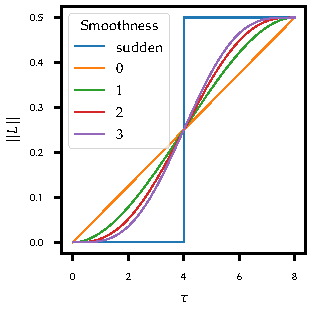
\includegraphics{figs/one_bath_mod/modulation_protocols_init.pdf}
  \caption{\label{fig:L_mod_init} The interaction is being switched on
    smoothly over a period of \(8\) time units by the use of
    smoothstep functions (\cref{sec:smoothstep}) of different
    orders. A sudden protocol is being included for reference.}
\end{figure}
In \cref{sec:pure_deph} we derived the short term behavior of the
interaction dynamics by neglecting the system Hamiltonian. Up to now
we only have looked at the scenario in which the interaction is
present from the beginning. Now we will briefly demonstrate a case
where the interaction is switched on smoothly as in
\cref{fig:L_mod_init}.

The model is otherwise the same as \cref{eq:one_qubit_model}, where we
have chosen \(α(0)=1.6\) and \(ω_{c}=1\) for all the simulations. Some
\(N=10^{4}\) trajectories have been computed for each simulation.

The smoothness parameter \(s\) regulates to which order the derivative
of the modulation is continuous at \(t=0\) and \(t=8\). The modulation
of the coupling allows for a change in total energy. This leads to a
partial compensation for the ``initial slip'' energy gain of the bath.

\begin{figure}[htp]
  \centering
  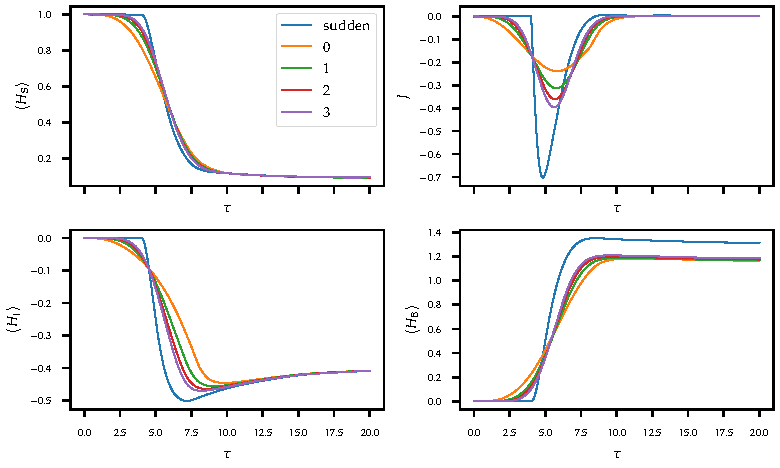
\includegraphics{figs/one_bath_mod/init_overview}
  \caption{\label{fig:init_energies}The relevant energy quantities for
    the different modulation protocols.}
\end{figure}
An overview over the bath, system and interaction energy, as well as
the bath energy flow can be found in \cref{fig:init_energies}. System
\(\ev{H_{\sys}}\) and interaction energy \(\ev{H_{\inter}}\) all
converge to the same values after some time, but the flows \(J\) and
bath energies are the greater, the faster we switch the coupling
on. The sudden switching of the interaction (blue) is the extreme
case, set apart by much greater interaction energies and a greater
final bath energy, as well as a much steeper initial peak in the flow.

The simulation with smoothness zero (yellow) exhibits a clear kink in
the bath energy flow and interaction energy curves at the time point
\(τ=8\), which reflects the lack of smoothness of the first derivative
of the modulation.

\cref{fig:init_total} shows that modulation protocols with a shallower
slope lead to a greater change in the total energy, compensating for
the negative interaction energy and leading to less initial
slip flow. Activating the coupling adiabatically will likely lead to a
complete avoidance of the initial slip. On the other hand, the system
and interaction dynamics will be intermingled increasingly with the
interaction buildup.

An interesting future application would be to simulate an adiabatic
transition from the non-interacting ground state into the interacting
ground state and a study of energy released in this way, especially
for strong coupling.

Circling back to the results of \cref{sec:pure_deph}, we can observe
in the right panel of \cref{fig:init_slip_mod} that the initial slip
flow is still valid for short times.  The actual flow (solid lines)
and the pure dephasing flow (dashed lines) agree initially but diverge
quite some time before peak flow.
\begin{figure}[htp]
  \centering
  \begin{subfigure}[t]{0.49\linewidth}
    \centering\captionsetup{width=.8\linewidth}
    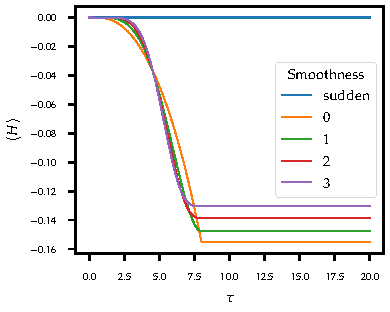
\includegraphics{figs/one_bath_mod/total_init}
    \caption{\label{fig:init_total}The total energy for different
      modulations. The slower the modulation, the more energy is
      released and the less energy is gained by the bath (see
      \cref{fig:init_energies}).}
  \end{subfigure}%
  \begin{subfigure}[t]{0.49\linewidth}
    \centering\captionsetup{width=.8\linewidth}
    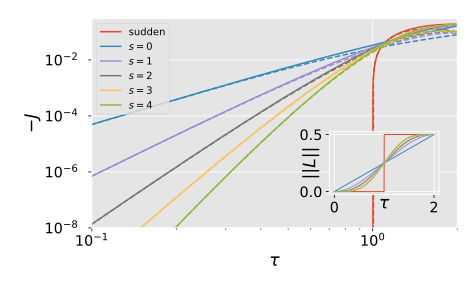
\includegraphics{figs/one_bath_mod/initial_slip_modcoup}
    \caption{\label{fig:init_slip_mod} The pure dephasing flow of
      \cref{eq:pureflowexpectation} and the exact flow. Initially, the
      flows coincidence, validating the earlier result. The flow peak
      heights and positions are being predicted incorrectly, but the
      initial slope and magnitude ordering are correct.}
  \end{subfigure}
  \caption{Total energy and flow for different interaction switching
    protocols.}
\end{figure}


\section{Conclusion}%
\label{sec:conclusion-1}
In this chapter we have validated the results of \cref{chap:flow} and
the fitness of the HOPS method for accessing bath related observables
using a direct comparison with the analytical solution of
\cref{chap:analytsol} and energy conservation in the spin-boson
model. We find that HOPS is well suited to obtain precise results
and that some trust can be placed in simulations that employ less
severe configurations, if numerical integration of the flow is
avoided. In all cases, the qualitative features of the energy
dynamics of the spin-boson model are captured very well.

We also explored the short term dynamics of the bath energy flow and
found that some light can be shed on it by considering the
approximation \(H_{\sys} = 0\). Further, the role of resonance and
bath memory time in the energy transfer performance of the zero
temperature spin-boson model was explored. The precise characteristics
of the energy flow depend strongly on the coupling strength and the
spectral density of the bath.

Now that we have built confidence in the method, we will turn to some
simple quantum-thermodynamical settings in
\cref{sec:therm_results}. There we will employ the capabilities of
HOPS to the fullest by treating multiple baths and (non harmonic)
modulation of the system and coupling.


\appendix
\chapter{Some Notes on HOPS}
\label{chap:hops_notes}
\section{Normalized HOPS}%
\label{sec:norm}

We introduce full HOPS vector \(Ψ = \qty(ψ, φ)\) which can be
decomposed into the zeroth hierarchy order state \(ψ\) and the
non-zero order states \(φ\).

The HOPS equations can then be written in an abstract manner as
\begin{equation}
  \label{eq:HOPS}
  \begin{aligned}
    \dot{ψ} &= F(ψ, φ), & \dot{φ} &= G(ψ, φ),
  \end{aligned}
\end{equation}
where \(c\cdot F(ψ, φ) = F(c\cdot ψ, c\cdot φ)\) and
\(c\cdot G(ψ, φ) = G(c\cdot ψ, c\cdot φ)\) for \(c\in\CC\)


The goal is to transform \(ψ \rightarrow \tilde{ψ}\) so that
\begin{equation}
  \label{eq:goal}
  \norm{\tilde{ψ}} = 1
\end{equation}
in a numerically stable manner.

Introducing the definitions \(\tilde{ψ} = \eu^{f(t)}ψ\) and
\(\tilde{φ} = \eu^{f(t)}φ\) with an
arbitrary\(f\colon \RR \rightarrow \CC\) we can begin to calculate
\begin{equation}
  \label{eq:normdgl}
  ∂_t\norm{\tilde{ψ}}^2 = \tilde{ψ}^† \qty(\dot{f}\tilde{ψ} +
  F(\tilde{ψ}, \tilde{φ})) + \cc = \dot{f} \abs{\tilde{ψ}}^2 +
  \tilde{ψ}^†F(\tilde{ψ}, \tilde{φ}) + \cc.
\end{equation}

We would now like to obtain \(∂_t\norm{\tilde{ψ}}^2 = 0\) as well as
\(\dot{f} > 0\) for \(\norm{\tilde{ψ}} < 1\), \(\dot{f} < 0\) for
\(\norm{\tilde{ψ}} > 1\) and \(\dot{f} = 0\) for
\(\norm{\tilde{ψ}}=1\), so that \(\norm{\tilde{ψ}} = 1\) becomes a
stable fix-point.

Observing \cref{eq:normdgl}, we conclude that our goals can be
achieved by demanding
\begin{equation}
  \label{eq:fdgl}
  \dot{f} = \frac{\tilde{ψ}^†F(\tilde{ψ},
    \tilde{φ})}{\norm{\tilde{ψ}}^2} + g\qty(\norm{ψ}^2)
\end{equation}
with \(g(0)=0\).

The first summand on its own would lead to norm conservation, \(∂_t\norm{\tilde{ψ}}^2 =
0\). The latter of our goals may be achieved by
choosing \(g(x) = \qty(1-x)\).

These choices lead to an altered HOPS equation
\begin{equation}
  \label{eq:normedhops}
  \dot{\tilde{Ψ}} = \qty[\frac{\tilde{ψ}^†F(\tilde{ψ},
    \tilde{φ})}{\norm{\tilde{ψ}}^2}+\qty(1-\norm{\tilde{ψ}}^2)]\mqty(\tilde{ψ}\\
  \tilde{φ}) + \mqty(F(\tilde{ψ},\tilde{φ}) \\ G(\tilde{ψ},\tilde{φ})).
\end{equation}

\section{Multiple Baths}
\label{sec:hops_multibath}

We generalize the NMQSD and HOPS to \(N\) baths for Hamiltonians of
the form~\cref{eq:multimodel}.


\subsection{NMQSD}
\label{sec:nmqsd}

Following the usual derivation of the NMQSD \cite{Diosi1998Mar}, we
switch to an interaction picture with respect to the \(H_\bath\)
leading to
\begin{equation}
  \label{eq:multimodelint}
  H(t) = H_\sys + ∑_{n=1}^N \qty[L_n^†B_n(t) + \hc],
\end{equation}
with \(B_n=∑_{λ} g_λ\nth a_λ\nth\eu^{-\iu ω_λ\nth t}\).

We will discuss the zero temperature case. The finite temperature
methods generalize straight forwardly to multiple baths.  Projecting
on a Bargmann (unnormalized) coherent state basis
\(\qty{\ket{\vb{z}^{(1)},\vb{z}^{(2)},\ldots}=
  \ket{\underline{\vb{z}}}}\) of the baths
\begin{equation}
  \label{eq:projected}
  \ket{ψ(t)} = ∫∏_{n=1}^N{\qty(\frac{\dd{\vb{z}\nth}}{π^{N_n}}\eu^{-\abs{\vb{z}}^2})}\ket{ψ(t,\underline{\vb{z}}^\ast)}\ket{\underline{\vb{z}}},
\end{equation}
where \(N_n\) are the number of oscillators in each bath.


We define
\begin{equation}
  \label{eq:processes}
  η^\ast_n(t) = {\qty(\vb{η}^\ast_t)}_n= -\iu ∑_λg_λ^{(n),\ast} z_λ^{(n),\ast}\eu^{\iu ω_λ\nth t}
\end{equation}
and using
\(\pdv{z_λ^{(n),\ast}}=∫\dd{s}\pdv{η^\ast_n(s)}{z_λ^{(n),\ast}}\fdv{η^\ast_n(s)}\)
we arrive at
\begin{equation}
  \label{eq:multinmqsd}
  ∂_tψ_t(\vb{η}^\ast_t) = -\iu H ψ_t(\vb{η}^\ast_t) +
  \vb{L}\cdot\vb{η}^\ast_tψ_t(\vb{η}^\ast_t) - ∑_{n=1}^N L_n^†∫_0^t\dd{s}α_n(t-s)\fdv{ψ_t(\vb{η}^\ast_t)}{η^\ast_n(s)},
\end{equation}
where \(α_n(t-s)= {\qty(\vb{α}(t-s))}_n=∑_λ\abs{g_λ\nth}^2\eu^{-\iu ω_λ\nth(t-s)}\) are the
zero temperature bath correlation functions. The equation
\cref{eq:multinmqsd} becomes the NMQSD by reinterpreting the
\(\vb{z}\nth\) as normal distributed complex random variables by
virtue of monte-carlo integration of \cref{eq:projected}. The
\(η^\ast_n(t)\) become homogeneous gaussian stochastic processes
defined through
\begin{equation}
  \label{eq:processescorr}
  \begin{aligned}
      \mathcal{M}(η^\ast_n(t)) &=0, & \mathcal{M}(η_n(t)η_m(s)) &= 0,
      & \mathcal{M}(η_n(t)η_m(s)^\ast) &= δ_{nm}α_n(t-s).
  \end{aligned}
\end{equation}

\subsection{Nonlinear NMQSD}
\label{sec:nonlin}

For the derivation of the lonlinear theory, the characteristic
trajectories of the partial differential equation of motion of
the Husimi-function
\begin{equation}
  \label{eq:husimi}
  Q_t(\underline{\vb{z}}, \underline{\vb{z}}^\ast) =
  \frac{\eu^{-\abs{{\underline{\vb{z}}}}^2}}{π^{∑_n N_n}}
  \braket{ψ(t, {\underline{\vb{z}}})}{ψ(t, {\underline{\vb{z}}}^\ast)}
\end{equation}
have to be determined.

Using \(∂_{\underline{\vb{z}}}\ket{ψ(t, {\underline{\vb{z}}}^\ast)} =
0\) and \(∂_{\underline{\vb{z}}^\ast}\bra{ψ(t, {\underline{\vb{z}}})} =
0\) because \(\ket{ψ(t, {\underline{\vb{z}}}^\ast)}\) is holomorphic
we derive
\begin{equation}
  \label{eq:husimimotion}
  ∂_tQ_t(\underline{\vb{z}}, \underline{\vb{z}}^\ast) = -i
  ∑_{n=1}^N\qty[∂_{z_λ^{(n), \ast}}\eu^{-\iu ω_λ\nth
    t}\ev{L^†_n}_tQ_t(\underline{\vb{z}}, \underline{\vb{z}}^\ast) - \cc],
\end{equation}
where \(\ev{L^†_n}_t = \mel{ψ(t, {\underline{\vb{z}}})}{L^†_n}{ψ(t,
  {\underline{\vb{z}}}^\ast)} / \braket{ψ(t, {\underline{\vb{z}}})}{ψ(t, {\underline{\vb{z}}}^\ast)}\).

The characteristics of \cref{eq:husimimotion} obey the equations of
motion
\begin{equation}
  \label{eq:characteristics}
  \dot{z}^{(n),\ast}_λ = \iu g_λ\nth \eu^{-\iu ω_λ\nth t} \ev{L^†_n}_t
\end{equation}
for the stochastic state labels.

The microscopic dynamics can in-turn be gathered into a shift of the
stochastic processes
\begin{equation}
  \label{eq:procshift}
  \tilde{η}_n^\ast(t) = η_n^\ast(t) + ∫_0^t\dd{s}α_n^\ast(t-s)\ev{L^†_n}_s
\end{equation}
and we obtain the nonlinear NMQSD equation
\begin{multline}
  \label{eq:multinmqsdnonlin}
  ∂_tψ_t(\tilde{\vb{η}}^\ast_t) = -\iu H ψ_t(\tilde{\vb{η}}^\ast_t) +
  \vb{L}\cdot\tilde{\vb{η}}^\ast_tψ_t(\tilde{\vb{η}}^\ast_t) \\-
  ∑_{n=1}^N
  \qty(L_n^†-\ev{L^†_n}_t)∫_0^t\dd{s}α_n(t-s)\eval{\fdv{ψ_t(\tilde{\vb{η}}^\ast_t)}{η^\ast_n(s)}}_{\vb{η}^\ast(s)
  = \vb{η}(\underline{\vb{z}}^\ast(t), s)}.
\end{multline}

The notation
\({\vb{η}^\ast(s) = \vb{η}(\underline{\vb{z}}^\ast(t), s)}\) means
that we replace the microscopic \(z_λ^{(n),\ast}\) in
\cref{eq:processes} with the shifted ones obeying
\cref{eq:characteristics} and evaluate the resulting function at \(s\).
This awkward construction can be remedied by the convolutionless
formulation. It plays no great role in the HOPS formalism.

\subsection{Multi Bath HOPS in Fock-Space Formulation}
\label{sec:multihops}

Following the usual derivation~\cite{RichardDiss} (but with a
different unitless normalization) and using an exponential expansion of the
BCFs \(α_n(τ)=∑_{\mu}^{M_n}=G_μ\nth\eu^{-W_μ\nth τ}\), we define
\begin{equation}
  \label{eq:dops}
  D_μ\nth(t) \equiv ∫_0^t\dd{s}G_μ\nth\eu^{-W_μ\nth (t-s)}\fdv{η^\ast_n(s)}
\end{equation}
and
\begin{equation}
  \label{eq:dops_full}
  D^{\underline{\vb{k}}} \equiv
  ∏_{n=1}^N∏_{μ=1}^{M_n}
  {\sqrt{\frac{\underline{\vb{k}}_{n,μ}!}{\qty(G\nth_μ)^{\underline{\vb{k}}_{n,μ}}}}
  \frac{1}{\iu^{\underline{\vb{k}}_{n,μ}}}}\qty(D_μ\nth)^{\underline{\vb{k}}_{n,μ}},
\end{equation}
as well as
\begin{equation}
  \label{eq:hierdef}
  ψ^{\underline{\vb{k}}} \equiv D^{\underline{\vb{k}}}ψ.
\end{equation}

Using
\begin{equation}
  \label{eq:commrelation}
  [D^\kmat(t),η_n^\ast(t)] =  \iu∑_{μ=1}^{M_n}
  \sqrt{\kmat_{n,μ}G\nth_μ} D^{\kmat -
    \mat{e}_{n,μ}}
\end{equation}
where \({\qty(\mat{e}_{n,μ})}_{ij}=δ_{ni}δ_{μj}\) we find after some algebra
\begin{multline}
  \label{eq:multihops}
  \dot{ψ}^\kmat = \qty[-\iu H_\sys + \vb{L}\cdot\vb{η}^\ast -
  ∑_{n=1}^N∑_{μ=1}^{M_n}\kmat_{n,μ}W\nth_μ]ψ^\kmat \\+
  \iu ∑_{n=1}^N∑_{μ=1}^{M_n}\sqrt{G\nth_μ}\qty[\sqrt{\kmat_{n,μ}}  L_nψ^{\kmat -
    \mat{e}_{n,μ}} + \sqrt{\qty(\kmat_{n,μ} + 1)}  L^†_nψ^{\kmat +
    \mat{e}_{n,μ}} ].
\end{multline}

The HOPS equations \cref{eq:multihops} can also be rewritten in an
especially appealing form \cite{Gao2021Sep} if we embed the hierarchy
states into a larger Hilbert space using
\begin{equation}
  \label{eq:fockpsi}
  \ket{Ψ} = \sum_\kmat\ket{\psi^\kmat}\otimes \ket{\kmat}
\end{equation}
where
\(\ket{\kmat}=\bigotimes_{n=1}^N\bigotimes_{μ=1}^{N_n}\ket{\kmat_{n,μ}}\)
are bosonic Fock-states.

Now \cref{eq:multihops} becomes
\begin{equation}
  \label{eq:fockhops}
  \begin{aligned}
    ∂_t\ket{Ψ} &= \qty[
                 \begin{aligned}
                 -\iu H_\sys + \vb{L}\cdot\vb{η}^\ast &-
                               ∑_{n=1}^N∑_{μ=1}^{M_n}b_{n,μ}^\dag b_{n,μ} W\nth_μ \\
                   &\qquad+
                 \iu ∑_{n=1}^N∑_{μ=1}^{M_n} \sqrt{G_{n,μ}} \qty(b^†_{n,μ}L_n +
                 b_{n,μ}L^†_n)
                 \end{aligned}
                 ] \ket{Ψ}\\
               &= \tilde{H}\ket{Ψ}
  \end{aligned}
\end{equation}

\section{Estimating the Norms of the Auxiliary States}
\label{sec:normest}

It is possible to find an (semi-rigorous) upper bound to the norms of
the auxiliary states. We will limit ourselves to one bath. The
generalization to multiple baths is straight forward.

Using \cref{eq:fockhops}, we can calculate
\begin{equation}
  \label{eq:normdiff}
  \begin{aligned}
    \iu ∂_t \norm{ψ^{\vb{k}}}^2
    &= \bra{Ψ}\ket{k}\bra{k}\tilde{H}\ket{Ψ} - \cc\\
    &= \qty(ψ^{\vb{k}})^†\bra{k}
      \qty[-\iu L η^\ast -\iu ∑_{μ=1}^{M}b_{μ}^\dag b_{μ} W_μ
      +∑_{μ=1}^{M} \sqrt{G_{μ}} \qty(b^†_{μ}L +
      b_μ L^†)]\ket{Ψ}- \cc\\
    &= \Bigg[-\iu \qty(ψ^{\vb{k}})^†L η^\ast ψ^{\vb{k}}
        -\iu ∑_{μ=1}^{M}k_μ W_μ \norm{ψ^{\vb{k}}}^2\\
        &\phantom{=}\quad -∑_{μ=1}^{M}\qty[\qty(ψ^{\vb{k}})^†\sqrt{G_{μ}k_μ}Lψ^{\vb{k}-\vb{e}_μ} +
        \qty(ψ^{\vb{k}})^†\sqrt{G_{μ}(k_μ+1)}Lψ^{\vb{k}+\vb{e}_μ} ]\Bigg]  - \cc.
  \end{aligned}
\end{equation}

We can now further treat the this expression to find the steady state
norms of the states.

Assuming generically that the term containing the stochastic process
\(η\) vanishes in the time average (as is the case for the steady
state) we will drop it in the following.

Terms of the form \(\Im(ψ^† O φ)\) may be estimated as follows
\begin{equation}
  \label{eq:genericest}
  \abs{\Im(ψ^† O φ)} \leq \norm{ψ} \norm{O φ} \leq \norm{ψ}\norm{O}\norm{φ},
\end{equation}
where the norm on the operator is the standard linear operator norm
\(\norm{O} = \max_{x\in \mathcal{H}}\frac{\ev{O}{x}}{\braket{x}}\).

We now endeavor to find from \cref{eq:normdiff} an estimate of the
steady state norm of \(ψ^{\vb{k}}\). To this end we assume that the
coupling to higher hierarchy states generically lowers the norm and is
therefore neglected. Using \cref{eq:genericest} we can estimate the
influence of the coupling to lower states, choosing the sign
so that the contribution to the norm is positive.

With this we obtain
\begin{equation}
  \label{eq:finalest}
  ∂_t \norm{ψ^{\vb{k}}}^2 = 0 = -∑_{μ=1}^{M}k_μ \Re[W_μ]
  \norm{ψ^{\vb{k}}}^2 +
  ∑_{μ=1}^{M}\abs{\sqrt{G_{μ}k_μ}}\norm{ψ^{\vb{k}}}\norm{ψ^{\vb{k}-\vb{e}_μ}}\norm{L}
\end{equation}
and therefore
\begin{equation}
  \label{eq:steadynorm}
  \norm{ψ^{\vb{k}}} =
  \frac{∑_{μ=1}^{M}\abs{\sqrt{G_{μ}k_μ}}\norm{ψ^{\vb{k}-\vb{e}_μ}}\norm{L}}{∑_{μ=1}^{M}k_μ \Re[W_μ]}.
\end{equation}


For the nonlinear method, the stochastic process obtains a shift whose
magnitude can be estimated as follows
\begin{equation}
  \label{eq:shiftestimate}
  \abs{η_{\mathrm{sh}}} \leq \norm{L} ∫_0^∞\dd{s}\abs{α^\ast(t-s)} \leq
  \norm{L} \sum_{μ=1}^M \frac{\abs{G_μ}}{\Re[W_μ]}.
\end{equation}
It is unclear how this shift should be treated. Simply adding it to
the denominator of~\cref{eq:steadynorm} lead to a breakdown of the
bound for numerical testing.  A better estimate should account for
this and also for the coupling to the lower orders foregoing the
recursive nature of the estimate.

The relation \cref{eq:steadynorm} is recursive
and break off at \(ψ^0\), the norm of which can be assumed to be unity
in the nonlinear method.

These ideas remain to be verified. Especially the assumptions should
be checked. For time dependent coupling, one may maximize the estimate
over all \(L(t)\).

As an illustration the validity of the bound for one specific model
see \cref{fig:normest_ω,fig:normest_δ}.
\begin{figure}[t]
  \centering
  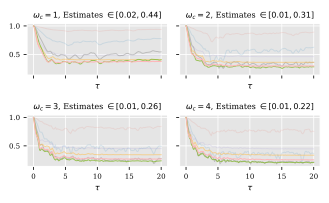
\includegraphics{figs/one_bath_syst/norm_estimate_omega}
  \caption{\label{fig:normest_ω} The maximum norm (for each time
    point) of the first hierarchy states for \(500\) trajectories
    subtracted from norm estimate and normalized by the norm estimate
    for a qubit coupled to single zero temperature ohmic baths
    \cref{eq:one_qubit_model} with varying \(ω_c\). The titles include
    the range of the norm estimates. For higher cutoff frequencies the
    BCF vanishes faster and the norm of the hierarchy states
    decreases. The opacity of the lines is proportional to their
    corresponding \(\abs{G_μ}\). The bound is tightest for the
    hierarchy states with the largest coupling.}
\end{figure}
\begin{figure}[p]
  \centering
  \plot{norm_est/norm_estimate_delta}
  \caption{\label{fig:normest_δ} The same as \cref{fig:normest_ω}, but
    for varying coupling strengths.}
\end{figure}

\subsection{Truncation Scheme}
\label{sec:truncsch}
The norm of the \(\vb{k}\)th hierarchy state scales like
\({1} / {\sqrt{\max_μk_μ}}\). This fact in itself, however, is not
too meaningful as the magnitude of the coupling to the lower hierarchy
states is
\begin{equation}
  \label{eq:couplingmag}
  M_{\vb{k}} = \norm{L} \norm{ψ^{\vb{k}}} \max_μ \abs{\sqrt{G_μk_μ}},
\end{equation}
which balances out the scaling.

Calculating \(M_{\vb{k}}\) explicitly and demanding it to be small
(compared to some energy scale) nevertheless gives a convergent
truncation scheme below a certain coupling strength.
Some basic experimentation has shown, that the cutoff parameter has to
be tuned and is not universally valid which is in accord with the
findings of \cite{RichardDiss}.

\section{Shifted Spectral Densities}
\label{sec:shift_sp}

\chapter{Additional Plots and Parameters\label{chap:plus_plots_params}}

\section{Plots}
\label{sec:plus_plots}

\subsection{Interaction Consisency Plots}
\label{sec:intercons}
\begin{figure}[H]
  \centering
  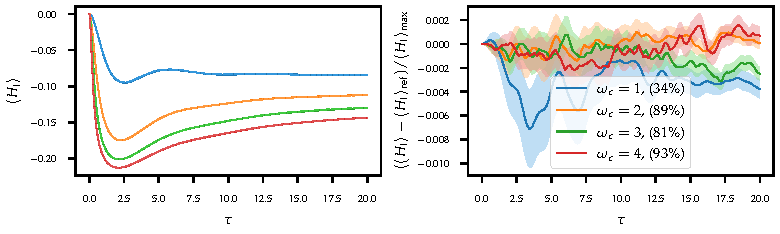
\includegraphics{figs/one_bath_syst/omega_interaction_consistency}
  \caption{\label{fig:omega_interaction_consistency}Interaction
    consistency plot for \cref{sec:one_bath_cutoff}, similar to
    \cref{fig:stocproc_systematics}.}
\end{figure}
\begin{figure}[H]
  \centering
  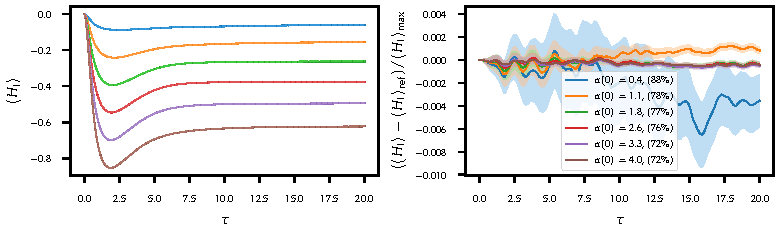
\includegraphics{figs/one_bath_syst/delta_interaction_consistency}
  \caption{\label{fig:delta_interaction_consistency}Interaction
    consistency plot for \cref{sec:one_bathcoup_strength}, similar to
    \cref{fig:stocproc_systematics}.}
\end{figure}

\subsection{Spectral Density Normalization}
\label{sec:spec_densities}
\begin{figure}[H]
  \centering
  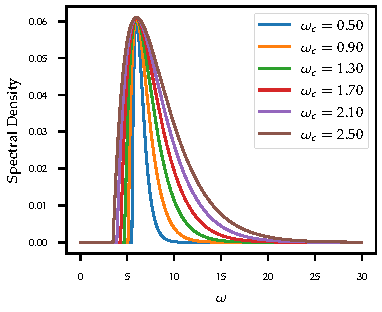
\includegraphics{figs/one_bath_mod/omega_sd_weak}
  \caption{\label{fig:omega_couplings_weak} Similar
    to \cref{fig:omega_couplings_and_energies} but for weaker coupling.}
\end{figure}


\subsection{More Plots for the Otto Cycle}
\label{sec:otto_plots}
\begin{figure}[H]
  \centering
  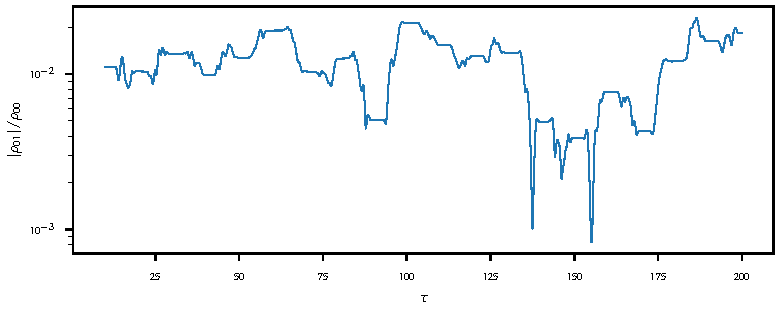
\includegraphics{figs/otto/coherences}
  \caption{\label{eq:otto_coherences} The coherences of the system
    state of the otto cycle in \cref{sec:otto}.}
\end{figure}
\begin{figure}[H]
  \centering
  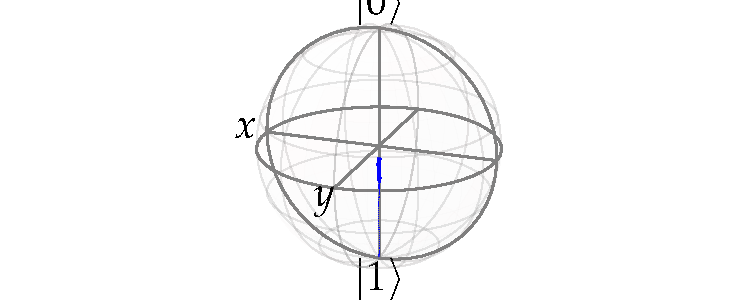
\includegraphics{figs/otto/bloch}
  \caption{\label{eq:otto_bloch} The system state of the model
    \cref{sec:otto} in the bloch sphere.}
\end{figure}

\section{Parameters}
\label{sec:plus_params}

\subsection{Modulation with a single Bath}
\label{sec:plus_mod_single}

\begin{table}
  \centering
  \begin{tabular}{lll}
    \hline
    $ω_c$              & $2$     & $2$    \\
    $α(0)$             & $0.7$   & $0.7$  \\
    $T$                & $5$     & $5$    \\
    $N$                & $10000$ & $2000$ \\
    $k_{\mathrm{max}}$ & $5$     & $5$    \\
    \hline
  \end{tabular}
  \caption{\label{tab:plus_friction}Additional parameters for
    \cref{fig:quant_frict}.}
\end{table}


\begin{table}
  \centering
  \begin{tabular}{lll}
    \hline
    $ω_c$              & $2$    & $2$    \\
    $α(0)$             & $0.7$  & $0.7$  \\
    $T$                & $5$    & $5$    \\
    $N$                & $1000$ & $1000$ \\
    $k_{\mathrm{max}}$ & $5$    & $5$    \\
    \hline
  \end{tabular}
  \caption{\label{tab:plus_system}Additional parameters for
    \cref{fig:quant_frict_sys_no_sys}.}
\end{table}

\begin{table}
  \centering
  \begin{tabular}{lllllll}
    \hline
    $ω_c$              & $0.50$     & $0.90$     & $1.30$     & $1.70$     & $2.10$     & $2.50$     \\
    $α(0)$             & $1.32$     & $1.42$     & $1.44$     & $1.33$     & $1.25$     & $1.37$     \\
    $T$                & $5.00$     & $5.00$     & $5.00$     & $5.00$     & $5.00$     & $5.00$     \\
    $N$                & $10000.00$ & $10000.00$ & $10000.00$ & $10000.00$ & $10000.00$ & $10000.00$ \\
    $k_{\mathrm{max}}$ & $5.00$     & $5.00$     & $5.00$     & $5.00$     & $5.00$     & $5.00$     \\
    BCF Terms          & $7.00$     & $7.00$     & $7.00$     & $7.00$     & $7.00$     & $7.00$     \\
    \hline
  \end{tabular}

  \caption{\label{tab:plus_omega}Additional parameters for the models in
     \cref{sec:extr_mem}.}
\end{table}


\begin{table}
  \centering
  \begin{tabular}{lllllll}
  \hline
   $ω_c$   & $ω_s$   & $α(0)$   & $T$    & $N$       & $k_{\mathrm{max}}$   & BCF Terms   \\
  \hline
   $1.00$  & $4.50$  & $0.78$   & $5.00$ & $1000.00$ & $7.00$               & $7.00$      \\
   $1.00$  & $4.62$  & $0.77$   & $5.00$ & $1000.00$ & $7.00$               & $7.00$      \\
   $1.00$  & $4.75$  & $0.76$   & $5.00$ & $1000.00$ & $7.00$               & $7.00$      \\
   $1.00$  & $4.88$  & $0.75$   & $5.00$ & $1000.00$ & $7.00$               & $7.00$      \\
   $1.00$  & $5.00$  & $0.74$   & $5.00$ & $1000.00$ & $7.00$               & $7.00$      \\
   $1.00$  & $5.12$  & $0.73$   & $5.00$ & $1000.00$ & $7.00$               & $7.00$      \\
   $1.00$  & $5.25$  & $0.72$   & $5.00$ & $1000.00$ & $7.00$               & $7.00$      \\
   $1.00$  & $5.38$  & $0.71$   & $5.00$ & $1000.00$ & $7.00$               & $7.00$      \\
   $1.00$  & $5.50$  & $0.70$   & $5.00$ & $1000.00$ & $7.00$               & $7.00$      \\
   $1.00$  & $4.50$  & $1.72$   & $5.00$ & $1000.00$ & $7.00$               & $7.00$      \\
   $1.00$  & $4.62$  & $1.70$   & $5.00$ & $1000.00$ & $7.00$               & $7.00$      \\
   $1.00$  & $4.75$  & $1.67$   & $5.00$ & $1000.00$ & $7.00$               & $7.00$      \\
   $1.00$  & $4.88$  & $1.65$   & $5.00$ & $1000.00$ & $7.00$               & $7.00$      \\
   $1.00$  & $5.00$  & $1.62$   & $5.00$ & $1000.00$ & $7.00$               & $7.00$      \\
   $1.00$  & $5.12$  & $1.60$   & $5.00$ & $1000.00$ & $7.00$               & $7.00$      \\
   $1.00$  & $5.25$  & $1.58$   & $5.00$ & $1000.00$ & $7.00$               & $7.00$      \\
   $1.00$  & $5.38$  & $1.56$   & $5.00$ & $1000.00$ & $7.00$               & $7.00$      \\
   $1.00$  & $5.50$  & $1.54$   & $5.00$ & $1000.00$ & $7.00$               & $7.00$      \\
  \hline
  \end{tabular}
  \caption{\label{tab:plus_tune}Additional parameters for the models in
     \cref{sec:modcoup_reso}.}
\end{table}


\printbibliography{}
\end{document}

%%% Local Variables:
%%% mode: latex
%%% TeX-master: t
%%% TeX-output-dir: "output"
%%% TeX-engine: luatex
%%% End:
